%%%%%%%%%%%%%%%%%%%%%%%%%%%%%%%%%%%%%%%%%%%%%%%%%%%%%%%%%%%%%%%%%%%%%%%%%%%%%
%%%% Preamble
%%%%%%%%%%%%%%%%%%%%%%%%%%%%%%%%%%%%%%%%%%%%%%%%%%%%%%%%%%%%%%%%%%%%%%%%%%%%%

%%%% The uwthesis.sty file relies on the memoir class!
%%%% You should be using the memoir class anyway; it makes life easier:
%%%% http://www.ctan.org/tex-archive/macros/latex/contrib/memoir/
\documentclass[oneside, letterpaper, 12pt, oldfontcommands]{memoir}
%%%% Import uwthesis.sty to get official formatting, then set your variables.
\usepackage{uwthesis}
\usepackage{cite}
\usepackage{graphicx}
\usepackage{textcomp}
\usepackage{rotating} % for sidewaystable
\usepackage{feynmp}
\usepackage{xspace}
\usepackage{amsmath}
\usepackage{helpers}
\usepackage{hyperref}
\usepackage[labelfont={bf,it},font={it}]{caption}
\DeclareGraphicsRule{.1}{mps}{*}{} %feynmp crap has .1 extension for some reason
\DeclareGraphicsExtensions{%
    .pdf,.PDF,% use PDFs first!
    .png,.PNG,%
    .jpg,.mps,.jpeg,.jbig2,.jb2,.JPG,.JPEG,.JBIG2,.JB2}

\graphicspath{ {figs/} {figs/BGs/} {figs/unfolded/} {figs/results/} }

\settitle{Discovery of the Higgs Boson and a Search for Beyond the Standard Model Physics in ZZ
Decays using the CMS Detector at the LHC}
\setauthor{Ian Ross}
\setdepartment{Physics}
\doctors % or \masters
\setgraddate{2013}
\setdefensedate{8.August.2013} % or whatever format you want

%%%% Members of the Final Oral Committee (FOC)
%%%% Give name, rank, and department
%%%% 
\setfoca{Sridhara Dasu}{Professor}{Physics} % <- Your advisor
\setfocb{Wesley Smith}{Bjorn Wiik Professor}{Physics}
\setfocc{Matt Herndon}{Professor}{Physics}
\setfocd{Vernon Barger}{Vilas Professor}{Physics}
\setfoce{Terry Millar}{Professor}{Mathematics}

%%%% Your abstract, used for the UMI abstract and in your front matter
\setabstract{%

A study of the $pp \rightarrow ZZ \rightarrow \ell\ell\ell\ell$ final state is
conducted using 19.6~\fbinv of 8 TeV proton-proton collisions at the LHC using the CMS
detector. The Standard Model $pp \rightarrow ZZ$ production cross section is
measured to be 
%$\sigma(pp\rightarrow ZZ) = 
$7.7^{+0.5}_{-0.5} \textrm(stat.) ^{+0.6}_{-0.5}
\textrm{(sys.)}  \pm 0.3 \textrm{(lumi)}~\textrm{pb} $. Evidence of a new
Higgs-like boson is observed with a significance of $6.1 \sigma$ at 126~GeV.
95\% confidence level upper limits are set on the neutral anomalous triple gauge
couplings; $-0.004 < f_4^Z < 0.004$, $-0.005 < f_4^{\gamma} < 0.005$, $-0.004 <
f_5^Z < 0.004$, and $-0.005 < f_5^{\gamma} < 0.005$.

}

%%%%%%%%%%%%%%%%%%%%%%%%%%%%%%%%%%%%%%%%%%%%%%%%%%%%%%%%%%%%%%%%%%%%%%%%%%%%%
%%%% Document
%%%%%%%%%%%%%%%%%%%%%%%%%%%%%%%%%%%%%%%%%%%%%%%%%%%%%%%%%%%%%%%%%%%%%%%%%%%%%

\begin{document}

% Tell the memoir class to set up lowercase roman for pagination, etc.
\frontmatter

%%%% Uncomment this to create a UMI abstract page.
%%%% If you are submitting electronically, however, this page is unnecessary.
% \theumiabstract

% The title page
\thetitlepage
\clearpage

% The copyright page, if you want to pay the fee and register copyright.
%\thecopyrightpage
%\cleardoublepage

% These above pages should not be counted, so we reset the counter to 1.
\setcounter{page}{1}

% An abstract may be required by your department.
\section{Abstract}
\uwabstract
\cleardoublepage

% Acknowledgements go here if you want to include them.
\section{Acknowledgements}
Acknowledgement is owed to many, and I deeply apologize for those who I've
left off this list (it's not intentional, I promise). Many thanks:

To Sridhara Dasu, Wesley Smith, and Matt Herndon for their endless support,
knowledge, and bountiful advice.

To Sascha Savin, for his patience, help, and ideas.

To Evan Friis and Maria Cepeda, for their wisdom and friendship.

To my fellow UW CMS students, past and present, for the support (be it
programming, physics, RCT, or life-related), and all the good times. Marc
Weinberg, Kira Grogg, Michalis Bachtis, Christos Lazaridis, Mike Anderson, Jeff
Klukas, Lindsey Gray, Jessica Leonard, Joshua Swanson, Isobel Ojalvo, Austin
Belknap, and all the rest -- I owe pieces of this work to each of you.

To my friends, in Madison and beyond, for always being there for me, even when
I was an ocean away.

To the HZZ4L Group, whose collective efforts are reflected in my work.

And to my family: my sister, Cameron, and my parents, Doug and Judy, for their
support and love. I couldn't have done it without you.


\clearpage

% Table of contents
\maxtocdepth{subsection}
\tableofcontents* % the * means that there isn't an entry for the TOC itself
\clearpage
\listoffigures  % if you have any figures
\clearpage
\listoftables   % if you have any tables

% Tell the memoir class to set up normal pagination, etc. for the main doc
\mainmatter

\setcounter{secnumdepth}{2} %allow subsubsection references

\input{Introduction}
\chapter{The Standard Model and Beyond}
\label{chapter:sm}
The Standard Model, the theoretical framework which describes fundamental
particles and their interactions, has a history rooted in the early-to-mid
twentieth century. At its core are two basic groups of particles,
\emph{fermions} and \emph{bosons}, along with three fundamental forces governing
their interactions. Throughout its growth over the last eighty years (as
outlined in~\ref{sec:overview}), the Standard Model has proven to be an
incredibly successful theory, with measurements validating its predictions to a
phenomenal accuracy. Despite its unprecedented level of success, the
Standard Model presents an incomplete description of the universe, as described
in~\ref{sec:shortcomings}, and the search continues for physics that falls
outside of the realm of this theory (\ref{sec:beyond}).

\section{Overview} \label{sec:overview}
The Standard Model unifies the most basic physical interactions into one
overarching framework.  The concept of such a unification can be traced back to
Einstein and beyond, but it is only in the last sixty years that the effort has
really taken shape. 

\subsection{Fundamental Particles} 
\label{sub:funpart}
There are two types of fundamental particles, \emph{fermions} and \emph{bosons}.
Ordinary matter is made up of \emph{fermions}, which carry half-integer spin.
Fermions can be further split into two sub-classes: quarks and leptons.  Quarks
are then classified into three generations of doublets, each generation
consisting of an "up-type" quark with charge $+2/3$ and a ``down-type'' quark
with charge $-1/3$. Quarks are never observed `alone' in nature, due to the laws
of quantum chromodynamics, as explained in~\ref{sub:forces}. Quarks are
susceptible to all three of the fundamental forces included in the Standard
Model -- the strong, weak, and electromagnetic forces. Via the strong force,
quarks form composite color-neutral particles known as \emph{hadrons}, either in
pairs (forming mesons), or in triplets (forming baryons). Protons and neutrons
are the most familiar particle in the hadron family and are composed of two
up-quarks and a down quark or two down-quarks and an up-quark respectively.

Leptons, the other type of fermion, differ in the fact that leptons carry no
color charge. As a result, they do not participate in any strong interactions.
However, the do participate in both electromagnetic (if charged) and weak
interactions. Like quarks, the lepton family is split into three generations,
consisting of the generational type (electron, muon, or tau -- \E, \M, or \T)
plus the doublet partner neutrino. 

\begin{table}[h]
\centering
\begin{tabular}{|c|c|c|c|c|}
\hline
\multicolumn{5}{|c|}{Generation 1} \\
\hline
Particle & Mass (eV/c$^2$) & Charge & T$^{3}$ & Forces\\
\hline
\E          &  5.11$\times$10$^5$   & $\pm 1$        & $+\frac{1}{2}$   & Electromagnetic, weak\\
$\nu_{e}$   &  $<$2.2               & 0              & $-\frac{1}{2}$   & Weak\\
u           &  $2.3\times10^6$      & $+\frac{2}{3}$ & $+\frac{1}{2}$   & Electromagnetic, weak, strong\\
d           &  $4.8\times10^6$      & $-\frac{1}{3}$ & $-\frac{1}{2}$   & Electromagnetic, weak, strong\\
\hline
\hline
\multicolumn{5}{|c|}{Generation 2} \\
\hline
Particle & Mass (eV/c$^2$) & Charge & T$^{3}$ & Forces\\
\hline
\M          & $1.05 \times10^8$     & $\pm 1$           & $+\frac{1}{2}$ & Electromagnetic, weak\\
$\nu_{\mu}$ & $< 1.70\times10^5$    & 0                 & $-\frac{1}{2}$ & Weak\\
c           & $1.3\times10^9$       & $+\frac{2}{3}$    & $+\frac{1}{2}$ & Electromagnetic, weak, strong\\
s           & $9.5\times10^7$       & $-\frac{1}{3}$    & $-\frac{1}{2}$ & Electromagnetic, weak, strong\\
\hline
\hline
\multicolumn{5}{|c|}{Generation 3} \\
\hline
Particle & Mass (eV/c$^2$) & Charge & T$^{3}$ & Forces\\
\hline
\T          & $1.77\times10^9$      & $\pm 1$           & $+\frac{1}{2}$ & Electromagnetic, weak\\
$\nu_{\tau}$& $< 1.55\times10^7$    & 0                 & $-\frac{1}{2}$ & Weak\\
t           & $1.74\times10^{11}$   & $+\frac{2}{3}$    & $+\frac{1}{2}$ & Electromagnetic, weak, strong\\
b           & $4.2\times10^9$       & $-\frac{1}{3}$    & $-\frac{1}{2}$ & Electromagnetic, weak, strong\\
\hline
\end{tabular}
\caption[Fermions and their properties.]{A summary of the generations of fermions and their mass, charge, weak
isospin ($T^{3}$ and the forces which act on them. Nota bene: all right-handed
particles have weak 0 isospin ($T^{3}=0$).}
\label{tab:fermions}
\end{table}

Integer- (or zero-) spin particles known as \emph{bosons} are the particles which
act as force-carriers, as described in~\ref{sub:forces}.  The most common of
these, the photon, is a massless spin-0 particle responsible for governing the
electromagnetic interactions between charged particles.  The \W and \Z bosons
carry the weak force and have charges of $\pm$ 1 and 0 respectively. 
The bosons are summarized in Table~\ref{tab:bosons}.  Gluons, the carriers of
the strong force, are, like photons, electrically neutral and massless. Unlike
the other force-carriers, however, the gluon carries a unit of color and
anti-color, meaning that it is able to self-interact. The implications of this
property are discussed in~\ref{sub:forces}

\begin{table}[h]
\centering
\begin{tabular}{|c|c|c|c|c|}
\hline
\multicolumn{5}{|c|}{Bosons} \\
\hline
Particle & Mass (eV/c$^2$) & Charge & T$^{3}$ & Forces\\
\hline
\Z & $91.2 \times 10^9$ & 0 & 0  & Weak\\
\W & $80.4 \times 10^9$ & $\pm 1$ & $\pm 1$ & Weak\\ 
\photon & 0 & 0 & 0 & Electromagnetic\\ 
g & 0 & 0 & 0 & Strong\\
\hline
\end{tabular}
\caption[Bosons and their properties.]{A list of the force-carrying bosons,
their mass, charge, weak isospin, and the force that they mediate.}
\label{tab:bosons}
\end{table}

\subsection{Fundamental Forces}
\label{sub:forces}
The concept that interactions between fundamental particles can be
attributed to mathematical constructs called fields extends to
Maxwell's formalism of electromagnetism, but it was Feynman, Tomanaga, and
Schwinger who first extended this formalism to the quantum
world. In his theory of quantum electrodynamics (QED,~\cite{Feynman:1950tx}), he
successfully described the electromagnetic interactions between charged
particles as an exchange of massless particles called photons. 

The weak force, carried by \W and \Z bosons, is responsible for those
interactions between fermions that involve charge and flavor changing (such as a
nucleus undergoing $\beta^{-} $ decay through the \Wm-mediated decay
\begin{equation*}
d \rightarrow u + e^{-} + \overline{\nu_{e}}
\end{equation*}

Both the weak and electromagnetic forces have interactions which are governed 
by probability amplitudes of the form:
\begin{equation*}
    \frac{g^4}{\left(q^2c^2-m^2c^4\right)^2}
\end{equation*}
where g is the force's coupling constant, q the momentum transfer of the
interaction, and m the mediating boson's mass. At higher energies (of the order
of $\sim100$~GeV, where the mass of the force-carrying bosons is dwarfed by the
momenta of the particles), the form of the two forces become identical (and
their relative strengths approach equality), suggesting a unification should be
possible between the two.

Sheldon Glashow, Abdus Salam, and Steven Weinberg \cite{Glashow:1961wk} provided
a mathematical basis to this idea, restructuring the forces into an \ewk
algebra.  Within this algebraic structure, the SU(2) operations act only upon
the fermions with left-handed \emph{chirality}, while the U(1) operations act on
those particles which carry hypercharge, Y. This quantum number relates to the
electrical charge, Q, and $T^3$ isospin component through the relation
\begin{equation*}
    Y = 2(Q-T^3)
\end{equation*}
This \ewk algebra describes four physical fields: three vector fields $W_\mu$ which couple to
the weak isospin current (with strength $g$) and one vector field, $B_\mu$ which
couples to the weak hypercharge current with strength proportional to $g'$.
Superposed, these fields describe the physical bosons:
\begin{equation}
\label{eqn:W}
    W_\mu^\pm = \sqrt{\frac{1}{2}}\left(W_\mu^1 \mp i W_\mu^2 \right) \\
\end{equation}
\begin{equation}
\label{eqn:Z}
    Z_\mu = -B_\mu \sin \theta_W + W_\mu^3 \cos \theta_W \\
\end{equation}
\begin{equation}
\label{eqn:g}
    A_\mu = B_\mu \cos \theta_W + W_\mu^3 \sin \theta_W \\
\end{equation}
Where~\ref{eqn:W} describes the weak charged current-carrying \W,~\ref{eqn:Z}
describes the weak neutral current-carrying \Z, and~\ref{eqn:g} describes the
electromagnetic force-carrying photon. $\theta_W$, known as the Weinberg angle,
carries information about the relative coupling strengths in the form
\begin{equation}
    \tan \theta_W = g'/g
\end{equation}.

The third fundamental force, the strong force, describes the interactions
between \emph{quarks} and \emph{gluons}. These are the fundamental particles
(further described in~\ref{sub:funpart}) which make up nuclear matter. The
theory of these interactions, known as quantum chromodynamics, was formulated
in the 1960s.

Because of the gluons' ability to interact with itself, the strong force is
unique in a number of respects. Most notably, the strong force grows stronger as
separation distance between color-charged particles increases. When a quark
sufficiently separates from another, the resulting energy is
enough for other quark-antiquark pairs to pop into existence from the vacuum.
The original quark then combines with these particles. This process, called
hadronization, is driven by \emph{asymptotic freedom} and restricts quarks from
being observed in an unbound state in nature. 

In the algebraic formulation of the Standard Model, the strong force
is represented by a \strong algebra, where C is indicative of the three color
charges (red, green, and blue). In any strong interaction, color must be
conserved, either through adding color and anticolor or one each of the red-
blue- and green- type particles (or anti-red, anti-blue, and anti-green-).

\subsection{Electroweak Symmetry Breaking}
The natural question, giving the unification between the electromagnetic and
weak forces at higher energies is: what causes the two to separate into distinct
forces at lower energies? It is clear that the difference is in the masses of
the force-carrying bosons, but there must be some physical process which gives
rise to the masses of the \W and \Z bosons, breaking the symmetries apparent in
the unified electroweak structure.

The mechanism for this symmetry breaking was proposed independently by
Higgs~\cite{PhysRevLett.13.508}, Englert and Brout~\cite{PhysRevLett.13.321}, and
Guralnik, Hagen, and Kibble~\cite{PhysRevLett.13.585}. The mechanism adds a Higgs
doublet to the electroweak model
\begin{equation*}
    \phi \equiv \left( \begin{array}{c} \phi^+ \\ \phi^0 \end{array} \right)
\end{equation*}
Adding to the potential terms of the form
\begin{equation*}
    V(\phi) = \mu^2\phi^\dagger\phi + \frac{\lambda^2}{2}(\phi^\dagger\phi)^2
\end{equation*}
For $\mu^2<0$, this potential produces a degenerate set of minimal values (see a
quantitative picture in Figure~\ref{fig:higgsPot}) and gives the Higgs field
$\phi$ a non-zero vacuum expectation value. This non-zero vaccuum expectation
value results in mass terms in the Lagrangian corresponding to the \W and \Z
boson.

\begin{figure}[h]
\centering
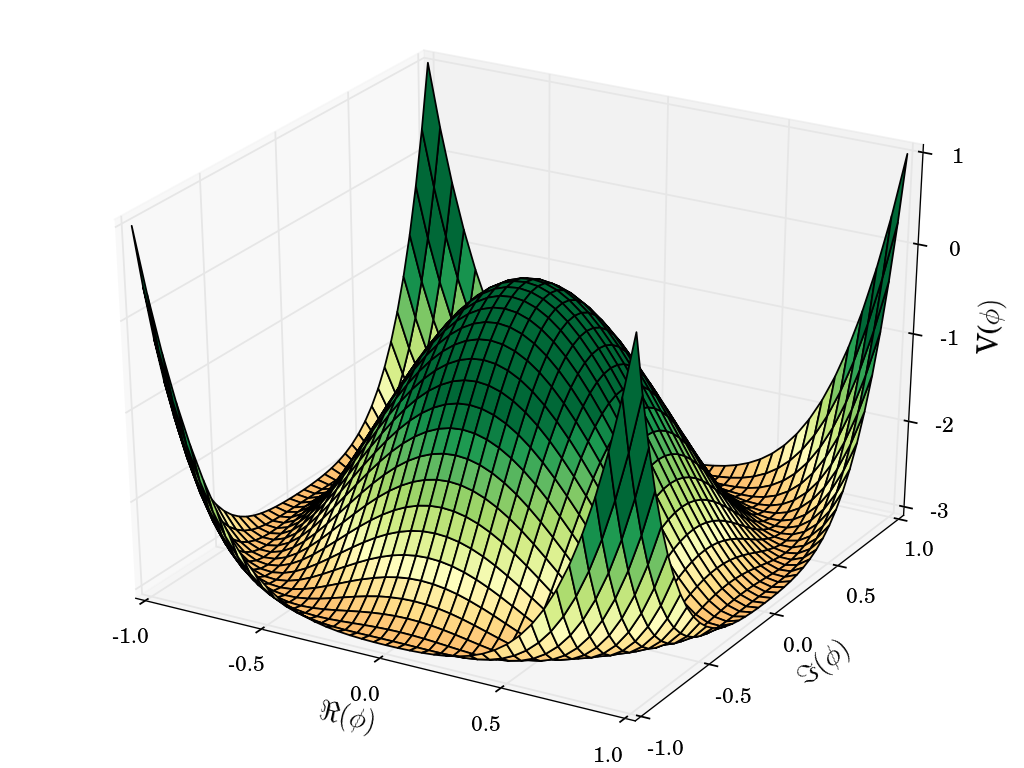
\includegraphics[width=\textwidth]{higgsPot} 
\caption[A quantitative picture of the Higgs potential.]{A quantitative picture
of the Higgs potential, with a ring of degenerate minima.}
\label{fig:higgsPot}
\end{figure}

Although this mechanism neatly explains how mass arises in certain aspects of the
electroweak structure, it is only very recently that a particle resembling the
Higgs boson has been observed (~\cite{CMS:higgsObs},~\cite{ATLAS:higgsObs}), and it has yet to be
conclusively shown whether the observed boson is the Standard Model Higgs or if
it is a Standard Model-like piece of another model. And, as explained
in~\ref{sec:shortcomings} there are certain aspects of the Higgs mechanism that
are left wanting.

\section{Proton-proton collisions}
\label{sec:protonCollisions}
The Large Hadron Collider (LHC) was built with the Higgs boson in mind. The
compositeness of the proton imparts the collisions with in non-trivial physical
ways. The \emph{uud} quark structure of the proton does not accurately describe
the way that the protons interact, as these \emph{valence} quarks are not the
objects that dictate the interactions. As the protons involved in the collisions
get higher and higher in energy, a larger fraction of the protons' momenta is
tied up in the so-called \emph{sea quarks}. These quarks, which can be of any
generation, arise spontaneously as $q\overline q$ pairs pop into existence from
gluons exchanged between the valence quarks. As a result, the LHC has a rich
field of possible initial states; $qq$, $q\overline q$, $qg$, and $gg$ processes
are all possible in the proton-proton collisions. 

Within the Standard Model, the final products in these interactions are governed
by the physical laws of the electroweak and QCD theories. The probability of a
given process occurring is typically expressed in terms of a \emph{cross
section}. The cross section, $\sigma$, is expressed in units of
area\footnote{The standard in particle physics is the \emph{barn}, defined as
$1~b = 10^{-24}~cm^2$} and can be calculated within the Standard Model (or
another relevant quantum field theory). 

These calculations, while often non-trivial, have been conducted for years and
have a well-established methodology. The most general form for a cross section
calculation at the LHC is:

\begin{equation}
    \sigma(pp \rightarrow P + X) = \frac{1}{3} \sum\limits_{q,q'} \int dx_1 dx_2
    f_1(x_1, Q^2) f_2(x_2, Q^2) \sigma_P(\hat s, \hat t, \hat u),
\end{equation}
where $f_1$ and $f_2$ are parton distribution functions and $\sigma_P$ is the
parton-level cross section arising from the matrix element for the process of
interest, P. These matrix elements are themselves calculated based on the rules
of the theory (specifically EWK in this analysis).  The production cross section
of a physical process is heavily dependent upon the forces, particles, and
energies involved. In general, at the energies probed at the LHC, particles
arising via QCD interactions are the most common (due to the high value of
\emph{$\alpha_{s}$}, the size of the strong force coupling.

The cross section provides an easy way to predict the relative rate of physical
processes:
\begin{equation}
    rate = \frac{dN}{dt} = \sigma \cdot \instlum
\end{equation}
Where N is the number of events produced and \instlum is the \emph{instantaneous
luminosity} of the proton beam collisions, explained further
in Section~\ref{section:theLHC}.


\section{Diboson Production} 
Within the Standard Model, a pair of Z bosons can be produced at the LHC either
through quark-antiquark interactions or through gluon interactions (involving a
quark loop)~\ref{fig:zzprod}. Because the standard model prohibits $ZZZ$ (or
$ZZ\gamma$) vertices, %why?
there is no s-channel contribution to the ZZ production
process of the type diagrammed in~\ref{fig:zzatgc}. The quark-antiquark
production mode is the dominant contribution, with the gluon-gluon mode
representing roughly 10\% of the overall cross section~\cite{Campbell:2011jv}.

\begin{figure}[h]
\centering
\unitlength = 1mm
\subfloat{
\begin{fmffile}{qq}
    \begin{fmfgraph*}(60,30)
    \fmfleft{i1,i2}
    \fmfright{o1,o2}
    \fmf{fermion,label=q}{i2,v2}
    \fmf{fermion,label=q}{v2,v1}
    \fmf{fermion,label=$\overline q$}{v1,i1}
    \fmf{photon,label=Z}{v1,o1}
    \fmf{photon,label=Z}{v2,o2}
    \end{fmfgraph*}
    \end{fmffile}
}
\subfloat{
    \begin{fmffile}{gg}
    \begin{fmfgraph*}(60,30)
    \fmfleft{i3,i4}
    \fmfright{o3,o4}
    \fmf{gluon,label=g}{i4,v4}
    \fmf{gluon,label=g}{i3,v3}
    \fmf{fermion,label=q}{v3,v4}
    \fmf{fermion,label=q}{v4,v5}
    \fmf{fermion,label=q}{v5,v6}
    \fmf{fermion,label=q}{v6,v3}
    \fmf{photon,label=Z}{v6,o3}
    \fmf{photon,label=Z}{v5,o4}
    \end{fmfgraph*}
    \end{fmffile}
}
\caption[Standard Model ZZ production]{Production of a ZZ diboson system in the LHC, through qq (left) and gg
production (right)}
\label{fig:zzprod}
\end{figure}

\begin{figure}[h]
\centering
\unitlength = 1mm
\subfloat{
    \begin{fmffile}{atgc}
    \begin{fmfgraph*}(60,30)
        \fmfleft{i6,i5}
    \fmfright{o5,o6}
    \fmf{fermion,label=q}{i5,v7}
    \fmf{fermion,label=$ \overline q$}{v7,i6}
    \fmf{photon,label=$Z,,\gamma$}{v7,v8}
    \fmfblob{0.16w}{v8}
    \fmf{photon,label=Z}{v8,o5}
    \fmf{photon,label=Z}{v8,o6}
    \end{fmfgraph*}
    \end{fmffile}
}
\caption[The SM-forbidden ZZZ (or ZZ$\gamma$ coupling.]{The SM-forbidden neutral triple vertex.}
\label{fig:zzatgc}
\end{figure}


% ------ Higgs production + decays ------
Additionally, a pair of Z bosons may be produced as the decay product of a Higgs
boson. The Higgs boson can be produced in a number of ways, but the dominant
methods are through gluon-gluon fusion and vector boson fusion (colloquially
called the gg and VBF production mechanisms). Additionally, it may be produced
in association with a vector boson (with final state VH) or through $t\overline
t$ fusion. Because the branching ratio of the final states considered in this
thesis are so small, the contributions from these two mechanisms are considered
negligible. Of the two sizable production modes, the $gg$ production
is the dominant mode at the LHC, due to the energies and properties of the
protons involved. The dominant Higgs production mechanisms (with decays to a ZZ
pair) is shown in Figure~\ref{fig:higgsProd}, with cross sections defined in
Table~\ref{tab:higgsProd}. 

\begin{figure}[h] 
\centering 
\unitlength = 1mm
\subfloat{
\subfloat{
    \begin{fmffile}{ggH}
    \begin{fmfgraph*}(60,30)
    \fmfleft{i1,i2}
    \fmfright{o3,o4}
    \fmf{phantom}{i1,v1,d1,o3}
    \fmf{phantom}{i2,v2,d3,o4}
    \fmffreeze
    \fmf{gluon,label=g,l.side=left}{i1,v1}
    \fmf{gluon,label=g,l.side=left}{i2,v2}
    \fmf{fermion,tension=0.5,label=$b,,t$,l.side=left}{v3,v1,v2,v3}
    \fmf{dashes,label=H}{v3,v4}
    \fmf{photon,label=Z}{v4,o3}
    \fmf{photon,label=Z}{v4,o4}
    \end{fmfgraph*}
    \end{fmffile}
}
\begin{fmffile}{vbfH}
    \begin{fmfgraph*}(60,30)
    \fmfleft{i1,i2}
    \fmfright{o1,zo1,zo2,o2}
    \fmf{phantom}{i1,v1,o1}
    \fmf{phantom}{i2,v2,o2}
    \fmffreeze
    \fmf{fermion,label=q,l.side=left}{i1,v1,o1}
    \fmf{fermion,label=q,l.side=left}{i2,v2,o2}
    \fmf{photon,label=$V$,l.side=left}{v1,v3}
    \fmf{photon,label=$V$,l.side=right}{v2,v3}
    \fmf{dashes,label=H}{v3,v4}
    \fmf{photon,label=$Z$,l.side=right}{v4,zo1}
    \fmf{photon,label=$Z$}{v4,zo2}
    \end{fmfgraph*}
    \end{fmffile}
}
\caption[Higgs$\rightarrow$ZZ production.]{The production mechanism of a ZZ system, from a Higgs boson. The $gg$
    (vector boson) fusion is depicted on the left (right).}
\label{fig:higgsProd}
\end{figure}

\begin{table}[h]
\centering
\begin{tabular}{|c|c|c|}
\hline
Production Mode & $\sigma_{8~TeV}$ (pb) & $\sigma_{7~TeV}$ (pb) \\
\hline
$gg \rightarrow H$              & 19.22 & 15.08\\
VBF                             & 1.568 & 1.211\\
WH                              & 0.6782 & 0.5576\\
ZH                              & 0.3843& 0.3077\\
$t\overline t$                  & 0.1271 & 0.0843\\
\hline
\end{tabular}
\caption[Higgs production cross sections at the LHC.]{Higgs boson production cross sections at 7 and 8 TeV for a mass of 126
    GeV.}
\label{tab:higgsProd}
\end{table}

The Higgs boson has well-defined decay characteristics within the Standard Model
(Fig.~\ref{fig:higgsBR}). At the mass of the observed Higgs-like boson
($\sim$126~GeV), the leading decay mode is to a $b\overline b$ pair, accounting
for approximately 56\% of Higgs decays. ZZ decays represent less than 3\% of
total Higgs decays, and only 1\% of those decay into four leptons. However,
given the high resolution with which the electrons and muons can be
reconstructed and the unmatchably clean signature of four leptons, the
$H\rightarrow ZZ \rightarrow \ell \ell \ell' \ell'$ represents a critical
channel in Higgs searches. %2.9% H->ZZ 

\begin{figure}[h]
\centering
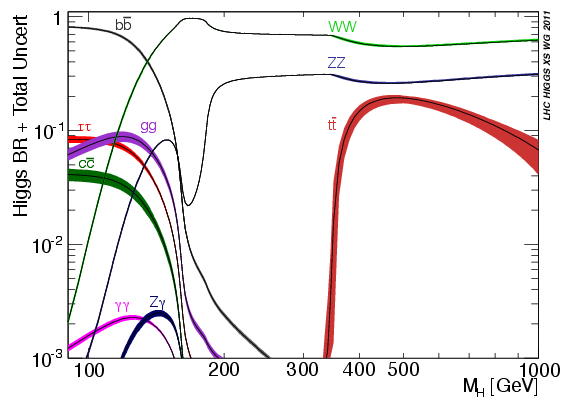
\includegraphics[width=\textwidth]{higgs-BR} %from https://twiki.cern.ch/twiki/bin/view/LHCPhysics/CrossSections
\caption{Higgs decays}
\label{fig:higgsBR}
\end{figure}

The cross sections for each of these ZZ production mechanisms is displayed in
Table~\ref{tab:Zprod}

\begin{table}[h]
\centering
\begin{tabular}{|c|c|c|}
\hline
Production Mode & $\sigma_{8~TeV}$ (pb) & $\sigma_{7~TeV}$ (pb) \\
\hline
$qq \rightarrow ZZ$ + $gg\rightarrow ZZ$ &  7.92   & 6.46 \\
%$gg \rightarrow ZZ$         & & \\
$ H (125~GeV) \rightarrow ZZ$ (total)  & 0.637 & 0.500\\
\hline
\end{tabular}
\caption[ZZ Production cross sections at the LHC.]{ZZ Production cross sections at 7 and 8 TeV. The Higgs production
mechanism includes all contributions (including associated production and
$t\overline t$ fusion).}
\label{tab:Zprod}
\end{table}

\Z bosons are unstable particles and decay into fermion-antifermion pairs. The
majority of these decays are into quarks which immediately decay hadronically.
The next leading Z decay is the decay mode to neutrino pairs, which escape the
detector without interaction. The third, and most relevant within the context of
this thesis, are the decays into lepton pairs. These decays represent roughly
10\% of all Z decays, as demonstrated in Table~\ref{tab:Zdecays}.

\begin{table}[h]
\centering
\begin{tabular}{|c|c|}
\hline
Decay Mode & Fraction (\%) \\
\hline
$e^+e^-$        & $3.363\pm0.004$   \\
$\mu^+\mu^-$    & $3.366\pm0.007$   \\
$\tau^+\tau^-$  & $3.370\pm0.008$   \\
Invisible       & $20.0\pm0.06$     \\
Hadrons         & $69.91\pm0.06$    \\
\hline
\end{tabular}
\caption[Breakdown of decay modes for the \Z boson.]{The branching ratios of the
most common decay modes of the \Z boson. Roughly 10\% of all created \Z bosons
decay leptonically, which is the mode of interest in this thesis.}
\label{tab:Zdecays}
\end{table}

\section{Shortcomings}
\label{sec:shortcomings}
Despite its great successes, the Standard Model is known to be at best an
incomplete theory. Pieces of the theory carry a conspicuously ad-hoc nature, as
the physical constants left floating must be adjusted in a fine balance in order
to cancel divergences in the theory. Similarly, the mechanism of electroweak
symmetry breaking has a non-zero vacuum expectation value only if the $\mu^2$
parameter is negative, which has no physical motivation.

The Standard Model also falls short at being a perfectly unified theory, as it has
little to say about the fourth fundamental force: gravity. Attempts to unify
the Standard Model as it stands today with gravitational forces prove incredibly
difficult, as the scale of the gravitational force is many orders of magnitude
smaller than the others, even at the high energy scales of unification.

Experimental evidence is mounting (~\cite{snoNeutrinoMixing,
superKNeutrinoMixing, dayaNeutrinoMixing}) which indicates
that neutrinos have mass, while the Standard Model in its form presented here
contains massless neutrinos.

The Standard Model, to some extent, seems to provide tension with today's
cosmological theories. It has no components explaining the cosmological phenomena
\emph{dark matter} and \emph{dark energy}. These objects, which compose 23\% and
72\% of the universe's energy content, respectively, have not been accounted for.
There is also no explanation as to why the matter in the universe is composed of 
`ordinary' matter, as opposed to antimatter. The two are suspected to have
existed initially in equal mixing, though only ordinary matter is seen today.

Finally, there's no indication of where the structures and classifications come
from. Why, for example, are there three generations of leptons and quarks
instead of four? Is the current mix of forces `final,' or is it possible to unite
all three forces into one? 

\section{Physics Beyond the Standard Model}
\label{sec:beyond}

Several attempts have been made to answer these some (or all) of these
questions, from the extensions of Supersymmetry, technical to a fully reimagined
grand unified theories, like string theory.  These  theories largely fall
outside of the scope of this thesis, but theories which predict new particles
with ZZ decays (such as those that predict a $Z'$ boson) or neutral triple gauge
couplings have ramifications explained below.
%\subsection{$Z'$ Bosons}
%todo: quick explanation of Z' bosons?

\subsection{Neutral Triple Gauge Couplings}
In the SM, ZZ production proceeds via the $t$- and $u$-channel
$q\overline q$ scattering diagrams, and via gluon-gluon fusion.  The presence of
anomalous neutral trilinear couplings (aTGCs) ZZZ and ZZ$\gamma$
would lead to a sizable enhancement of ZZ final states via $s$-channel
$q\overline q$ scattering as in~\ref{fig:zzatgc}.  A model featuring such
couplings can be constructed by means of an effective
Lagrangian~\cite{Hagiwara:1987tv}.  In this parametrization, two ZZZ couplings
and two ZZ$\gamma$ couplings are allowed by electromagnetic gauge invariance and
Lorentz invariance for on-shell Z bosons.  The form of the vertex function may
be written as: 
\begin{equation}
    \Gamma^{\alpha,\beta,\mu}_{V} = \frac{\hat s-m_V^2}{m_Z^2}\left(
        i f_4^V \left( P^\alpha g^{\mu\beta} \right ) + 
    i f_5^V\epsilon^{\mu\alpha\beta\rho}\left ( q_1-q_2\right)_\rho \right)
\end{equation}.
The couplings are parametrized by two CP-violating (
\ffour ) and two CP-conserving ( \ffive ) complex parameters, all of which are
zero at tree level in the Standard Model (as \ffive~breaks parity conservation).

In general, these couplings do not necessarily conserve partial wave unitarity
at high center-of-mass energies (due to their dependence on$\hat s$). In
previous literature, the $\hat s$ dependence is treated using a form factor,
\begin{equation*} 
    f_i^V(\hat s) = \frac{f_{i0}^V}{\left(1+\frac{\hat s}{\Lambda^2_{NP}}\right)^n}
\end{equation*}
where $\Lambda_{NP}$ is the energy scale at which the new physics manifests
itself and $f_{i0}^V$ is the bare value of the coupling. However, the coupling
values being considered ($\sim0.06$) are unitarity safe through our sensitive
region ($m_{4l} < 1.5~TeV$~\cite{zralek}), and, as a result, no form factor is
assumed. The limits presented in this analysis can thus be interpreted as
restrictions on the `bare' $f_{i0}^V$ couplings.

\subsubsection{Observable manifestations of aTGCs} 
Any indications that these couplings are non-zero are an immediate signal of
physics beyond the standard model. The phenomenological effects are well
described by theorists (for example, \cite{Baur:2000vi}).  The most immediate
effect of anomalous couplings in an increase in the ZZ production cross section,
which would result in a higher-than-anticipated number of observed events.
Additionally, the coupling effects shape the kinematics of the event, becoming
especially pronounced at higher energies. Within the context of this thesis, the
most relevant manifestations are the broad increases in the system's invariant
mass, increases in the \Z transverse momenta, and increased lepton transverse
momenta. The effects on the boson and lepton are exemplified in
figure~\ref{fig:atgcEffects}, reproduced from~\cite{Baur:2000vi}.

Because the effects of the couplings \ffour and \ffive enter the matrix elements
identically, it is impossible to distinguish the two based solely on the effects
explained above. However, it is feasible to comb out some more distinction
between the various couplings given their differing impact on helicity
amplitudes. Specifically, the \ffive couplings produce terms that interfere with
the helicity amplitudes produced by Standard Model couplings. Finally, if
evidence of these couplings were to be found, separation between the leptons
coming from a Z boson (both in the spatial separation and the azimuthal angle
between them) can provide subtle clues to the type (and possibly sign) of the
coupling. The effects can be see in figure~\ref{fig:atgcAngEffects}, reproduced
from~\cite{Baur:2000vi}.

\begin{figure}[h]
\centering
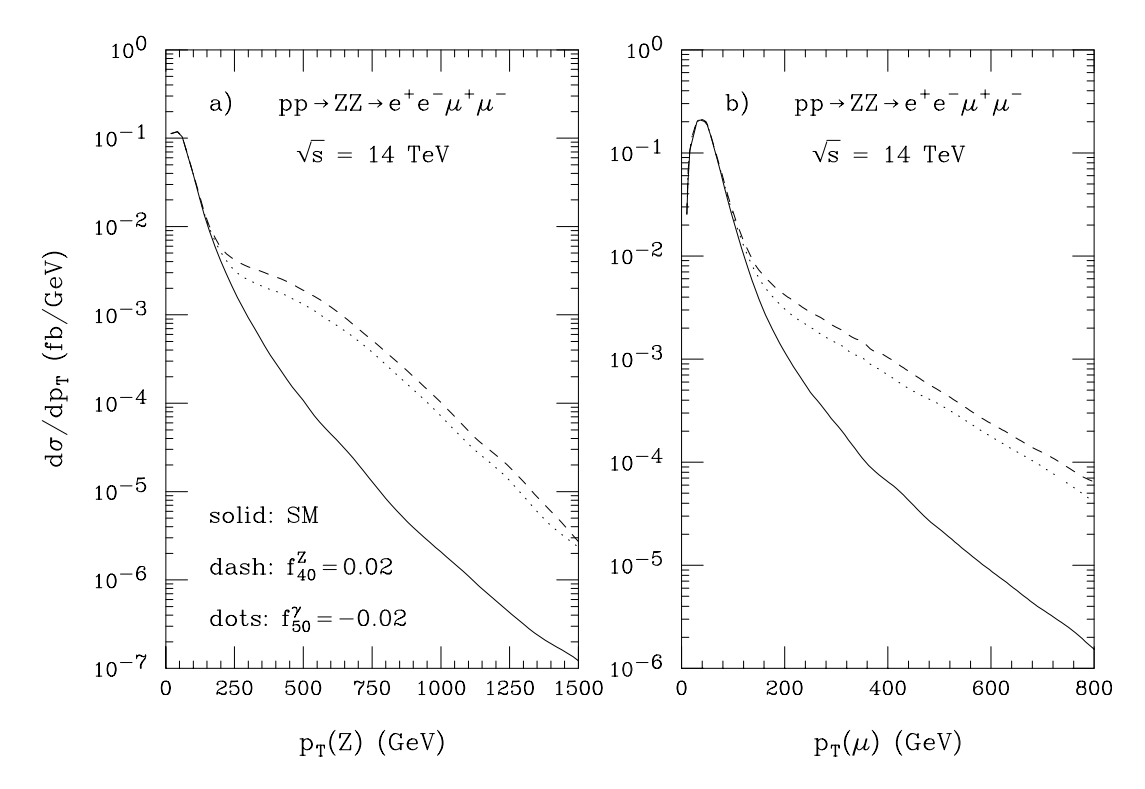
\includegraphics[width=\textwidth]{atgcEffects} 
\caption[Phenomenological effects of aTGCs on boson and lepton
$p_T$.]{Phenomenological effects of aTGCs on boson and lepton $p_T$, reproduced
from~\cite{Baur:2000vi}. Note especially the pronounced high-energy tails
produced by the anomalous couplings.}
\label{fig:atgcEffects}
\end{figure}

\begin{figure}[h]
\centering
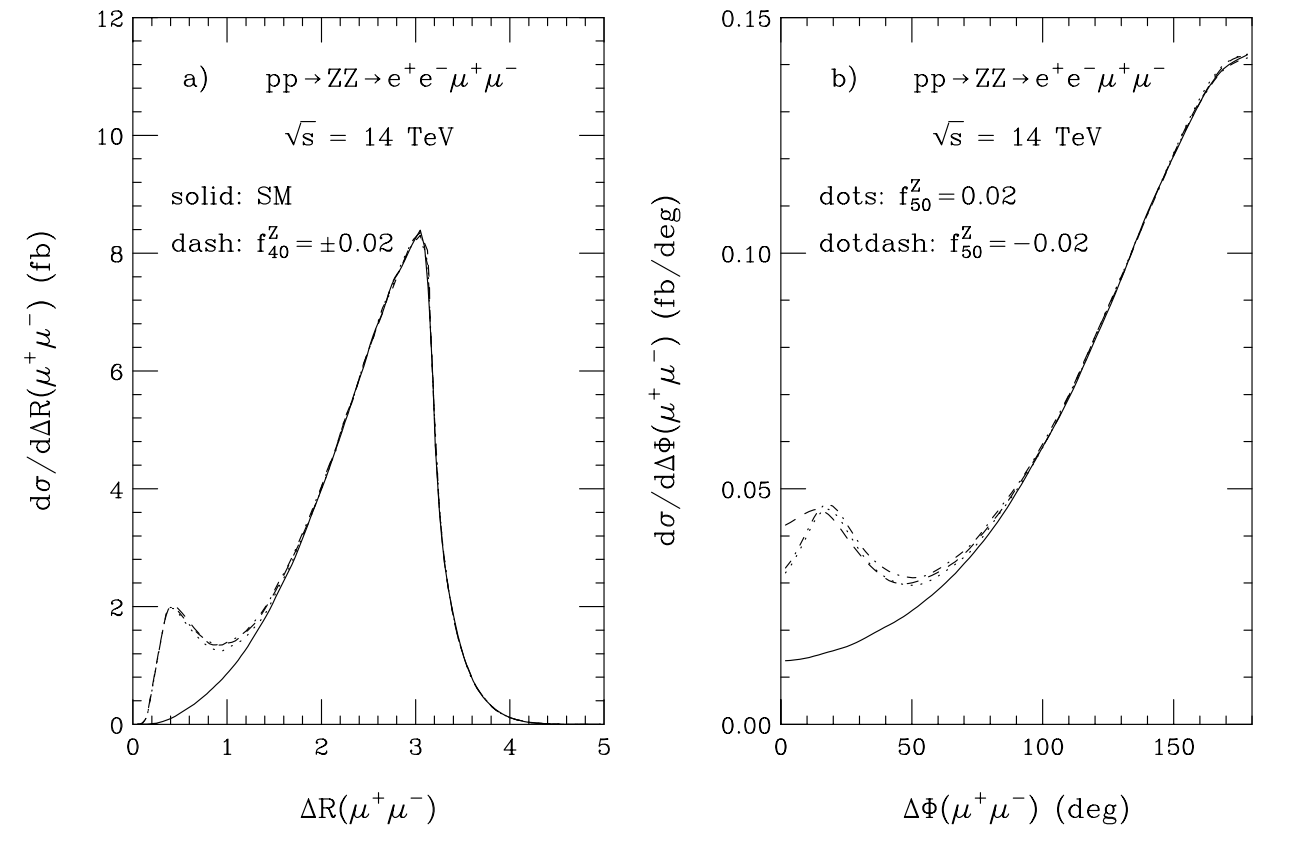
\includegraphics[width=\textwidth]{atgcAngEffects} 
\caption[Phenomenological effects of aTGCs on lepton
separation.]{Phenomenological effects of aTGCs on the separation between leptons, reproduced
from~\cite{Baur:2000vi}. The type, size, and sign of the coupling create slight
differences in the azimuthal angle distribution. Reproduced
from~\cite{Baur:2000vi}.}
\label{fig:atgcAngEffects}
\end{figure}

%todo: what theories predict aTGCs? How would ruling them out change things?

\chapter{Previous Results}
\label{chapter:previous}

\section{Observations and properties of the \Z boson}
The first indirect experimental evidence for the \Z boson was first observed at the
Gargamelle detector at CERN~\cite{Hasert:1973uq} in 1973. The experiment
consisted of passing a neutrino beam through a liquid bubble chamber and looking
for evidence of neutral currents in the form of electron-neutrino scattering:

\begin{equation*}
\overline{\nu}_{\mu} + e^- \rightarrow \overline{\nu}_{\mu} +  e^- \newline
\end{equation*}
\begin{equation*}
\nu_{\mu} +  e^- \rightarrow \nu_{\mu} +  e^-
\end{equation*}
Of the 735,000 pictures analyzed, one was characteristic of a neutral current
interaction, and is regarded as the first experimental evidence of the \Z boson.

The first direct evidence of the particle came almost a full 10 years later, in
1983, at CERN's Super Proton Synchrotron (SPS). The UA1 experiment observed four
events indicative of a $\Z\rightarrow e^+e^-$ decay and one $\Z\rightarrow
\mu^+\mu^-$ event, with invariant masses consistent with the SM prediction of
91.2 GeV\cite{UA1:Zobs}. The UA2 experiment corroborated the discovery soon
after.

Although the experiments at the SPS were able to provide the first evidence of
the \Z boson, it was not until the clean collisions recorded by the experiments
at CERN's Large Electron-Positron (LEP) collider that accurate measurements of
the boson's properties could be made in 1990. The energy of the collider, combined with
the clean environment of electron-positron collisions, made the experiments at
LEP a veritable factor of weak bosons. When coupled with data from the SLAC
Large Detector (SLD) at the Stanford Linear Collider, the electroweak sector was
fleshed out in intricate detail.  Unparalleled measurements of mass, total and
partial decay widths, coupling constants, and searches for new decay modes and
anomalous coupling modes were conducted at the LEP and SLAC experiments. The
results were superb validations of the Standard Model predictions, with mass
measurement and widths measured with per-mil accuracy.~\cite{lepSLD:zPhys}:

\begin{equation*}
    m_Z = 91.91875 \pm 0.0021 GeV \\
\end{equation*}
\begin{equation*}
    \Gamma_Z = 2.4952 \pm 0.0023 GeV
\end{equation*}
\begin{equation*}
    sin^2 \theta_W = 0.23153 \pm 0.00016
\end{equation*}

Experiments the Tevatron (especially during its Run II phase from 2001 to 2011)
repeated these measurements within the context of 1.96~GeV $p\overline p$
collisions, with cross-section and weak-mixing angles fully consistent with
Standard Model expectations~\cite{cdf:weakMixingAngle, d0:weakMixingAngle}


\section{Diboson Production}
ZZ diboson events were first observable at the LEP experiments when the $e^+e^-$
center of mass energy exceeded the ZZ kinematic threshold. ALEPH, DELPHI, L3,
and OPAL reported ZZ production cross sections fully consistent with Standard
Model Expectations~\cite{ALEPH:zz, DELPHI:zz, L3:zz, OPAL:zz}.

Because the $ZZ\rightarrow4\ell$ final state has such a low branching ratio,
previous experiments have observed a statistically limited sample of $4\ell$
events.  The latest Tevatron results include only a handful in each
detector~\cite{CDF:zz, D0:zz}. %, as evidenced in Figure~\ref{fig:tevatronZZ}.


%\begin{figure}[h]
%\centering
%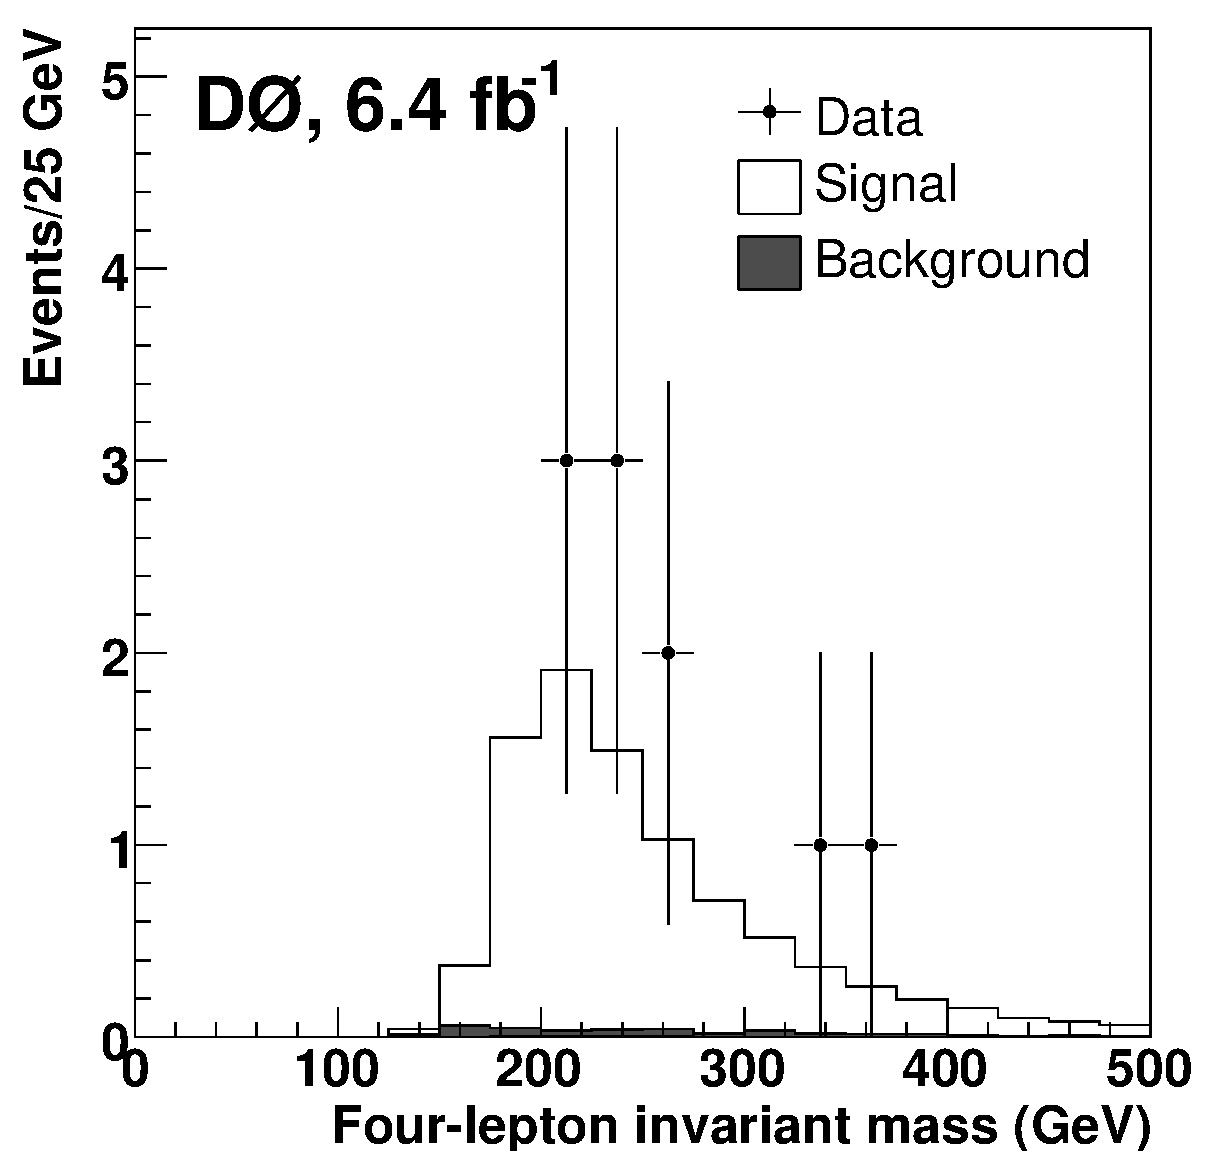
\includegraphics[width=0.45\textwidth]{d0_4lmass} %from http://www-cdf.fnal.gov/physics/ewk/2013/ZZ_97fb/ZZ4l.html
%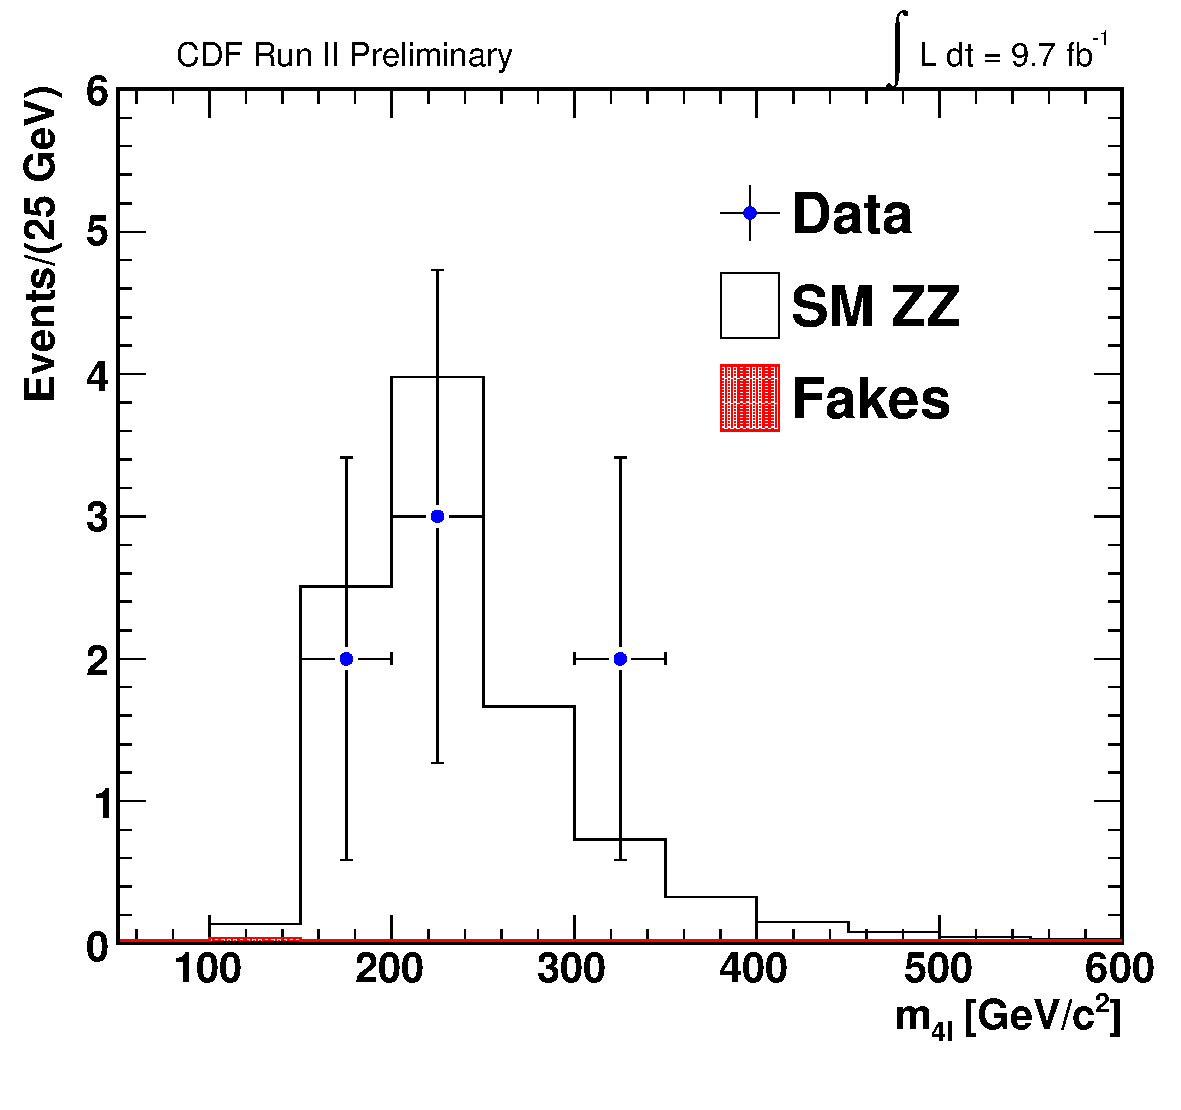
\includegraphics[width=0.45\textwidth]{cdf_4lmass} %from http://www-d0.fnal.gov/Run2Physics/WWW/results/final/EW/E11A/
%\caption[Tevatron observations of ZZ$\rightarrow$4l events.]{Observed four-lepton invariant mass for the Tevatron experiments. The
%data represent 6.4 \fbinv and 9.7 \fbinv of 1.96 TeV $p\overline p$ collisions
%at D0 and CDF (left and right, respectively).}
%\label{fig:tevatronZZ}
%\end{figure}

\section{Higgs Limits}
Experiments have been keen to observe the Higgs boson since its inception in the
1950s \cite{PhysRevLett.13.508, PhysRevLett.13.321, PhysRevLett.13.585}. While
the evidence remained elusive until the summer of 2012, the regions of possible
Higgs mass were constrained to ever-tighter regions of phase space.

After running from 1989-2000, the experiments at the Large Electron-Positron
(LEP) at CERN combined their direct searches to set a lower bound on the Higgs
Mass of 114.4 GeV~\cite{LEP:higgsLim} at 95\% Confidence level (CL).

Using the combined data from the LEP, SLC, and Tevatron experiments, a combined
fit to electroweak parameters was able to set an upper mass limit of 158
GeV~\cite{Grunewald:1313716}. %explain more?

Direct searches at the Tevatron ruled out $100 < m_H < 103$~GeV and
$147 < m_H < 180$~GeV at the 95\% confidence level, while reporting a broad
access of with a 2.9$\sigma$ significance~\cite{fnal:higgs}.

\section{Higgs Searches at the Large Hadron Collider}
The LHC was built with the Higgs boson in mind. As mentioned
in~\ref{sec:protonCollisions}, the proton-proton collisions provide an enhanced
rate of Higgs production, with expectations of either discovering the Higgs
boson at any mass, should it exist, or ruling out the mechanism entirely.

, with capability to produce Higgs boson, if it exists,
in sufficient quantity for any mass enabling a discovery or excluding the
mechanism itself.

Data taken at 7 TeV collision energy in the first two years of running left only
a small section of mass space for the Higgs boson. The first 5
\fbinv of data collected at 7~TeV allowed both the ATLAS and CMS experiments to carve out
a large portion of mass exclusion.  ATLAS ruled out (at 95\% CL) the masses
between 111.4-116.6, 119.4-122.1, and 129.2-541 GeV. CMS excluded from 127-600
GeV. By the time that the LHC was turned on again in 2012 (at 8 TeV
center-of-mass energy), only masses between 122.1 and 127 GeV had not been ruled
out at the 95\% CL. By the middle of the summer of 2012, the experiments had
gathered an additional 5 \fbinv at the higher energy and were able to announce,
on July 4, statistically significant evidence of a new
boson~\cite{cms:HiggsObs, atlas:HiggsObs}. Running through the end of 2012
produced another 15 \fbinv for the experiments, allowing each to begin to
characterize the particle. By all standards, the discovery does indeed look to
be the revered Higgs boson~\cite{ATLAS:higgsProperties, CMS:higgsProperties}.

%table with all limits

\section{Searches for neutral triple gauge couplings}
Searches for anomalous neutral triple gauge couplings have been performed at
LEP2~\cite{ALEPH, DELPHI, OPAL, LEPWG, L3}, the Tevatron~\cite{D0, CDF}, and
the LHC~\cite{ATLAS, ATLAS2, CMS}. Since no direct evidence has been
observed, all results are quoted as upper limits. The most stringent limits to 
date were set by the author and the CMS collaboration \cite{CMS}. The
limits on each of the couplings are summarized in~\ref{tab:atgcPrevLimits}.

\begin{table}[htbp]
\footnotesize
\centering
\setlength{\tabcolsep}{5pt}
\begin{tabular}{|c|c|c|c|c|l|}
\hline
Experiment & $f_4^Z$ & $f_4^\gamma$ & $f_5^Z$ & $f_5^\gamma$ &  Comments
\\
\hline
\hline
ALEPH~\cite{ALEPH}           & [-0.60;0.61] & [-0.40;0.36] & [-1.22;1.10] & [-0.81;0.79] &
2D fit results\\
\hline
DELPHI~\cite{DELPHI}          & [-0.40;0.42] & [-0.23;0.25] & [-0.38;0.62] & [-0.52;0.58] &
 \\
\hline
L3~\cite{L3}              & [-1.9;1.9] & [-1.1;1.2] & [-5.0;4.5] & [-3.0;2.9] 
& $\surd{s} = 189$ GeV\\
\hline
OPAL~\cite{OPAL}         & [-0.45;0.58] & [-0.32;0.33] & [-0.94;0.25] & [-0.71;0.59] & \\
\hline
LEP WG~\cite{LEPWG}               & [-0.30;0.30] & [-0.17;0.19] & [-0.34;0.38] & [-0.32;0.36]
& LEP combination\\
\hline
\hline
CDF~\cite{CDF}         & [-0.12;0.12] & [-0.10;0.10] & [-0.13;0.12] & [-0.11;0.11] &
$\Lambda$=1.2 TeV \\
\hline
D0~\cite{D0}          & [-0.28;0.28] & [-0.26;0.26] & [-0.31;0.29] & [-0.20;0.28] &
\begin{tabular}{@{}c@{}} $\sim 1$ \fbinv, \\ $\Lambda$=1.2 TeV \end{tabular} \\
\hline
\hline
ATLAS~\cite{ATLAS}           & [-0.12;0.12] & [-0.15;0.15] & [-0.13;0.13] & [-0.13;0.13] &
\begin{tabular}{@{}c@{}} $\sim 1$ \fbinv, \\$\Lambda$=2 TeV \end{tabular}\\
\hline
ATLAS~\cite{ATLAS}           & [-0.07;0.07] & [-0.08;0.08] & [-0.07;0.07] & [-0.08;0.08] &
\begin{tabular}{@{}c@{}} $\sim 1$ \fbinv,\\ $\Lambda$=inf \end{tabular}\\
\hline
ATLAS~\cite{ATLAS2}          & [-0.019,0.019] & [-0.022,0.023] & [-0.020,0.019]
& [-0.023,0.023] &
\begin{tabular}{@{}c@{}} 4.6 \fbinv,\\ $\Lambda$=3~TeV \end{tabular}\\
\hline
ATLAS~\cite{ATLAS2}          & [-0.013,0.013] & [-0.015,0.015] & [-0.013,0.013]
& [-0.016,0.015] &
\begin{tabular}{@{}c@{}} 4.6 \fbinv,\\ $\Lambda$=inf \end{tabular}\\
\hline
CMS~\cite{CMS}           & [-0.011;0.012] & [-0.013,0.015] & [-0.012,0.012] &
[-0.014,0.014] &
\begin{tabular}{@{}c@{}} $\sim 5$ \fbinv, \\$\Lambda$=inf \end{tabular}\\
\hline
\end{tabular}
\vspace{0.5cm}
\caption[Summary of existing 95\% C.L  for neutral aTGCs.]{Summary of existing 95\% C.L. intervals for the neutral aTGC $f_4^Z$,
$f_4^\gamma$, $f_5^Z$ and $f_5^\gamma$.
}
\label{tab:atgcPrevLimits}
\end{table}

\chapter{Experimental Overview of the LHC and CMS}

\label{chapter:expOverview}
The Large Hadron Collider (LHC) is the latest (and most powerful) collider built
to date. It sits beneath the French-Swiss border outside of Geneva, in the
tunnels that were originally used to house LEP. It was designed for
proton-proton collisions, with designed center-of-mass energies of up to 14 TeV.
These design center of mass energies will not be reached until after a series of
hardware updates which are currently underway. This thesis uses instead the
collision data collected at 7 and 8 TeV center-of-mass energies.

The LHC houses 4 major detectors, in addition to a handful of secondary
experiments. The Compact Muon Solenoid (CMS) and A Toroidal LHC Apparatus
(ATLAS) are general-purpose detectors that sit roughly across from each other on
the main proton ring. LHCb is a detector specializing in b-physics (the physics
of mesons containing bottom quarks). The fourth major experiment is the A Lead
Ion Collider Experiment, or ALICE. This detector is designed for primary
operation during the LHC's heavy ion collision mode. Additional experiments,
such as TOTEM and LHCf, are smaller in scale, but aim for important measurements
(these in particular aim, respectively, for total pp cross section measurements
and forward neutral pion measurements).

The operation of the LHC is outlined in Section~\ref{section:theLHC}, while CMS
and its subcomponents are explained in detail in Section~\ref{section:cms}.

\section{Definitions of Terminology}

The geometry of the CMS detector is defined such that the $\hat x-$axis points
toward the center of the ring, and the $\hat y-$axis points upward. The $\hat
z-$axis, then, points in the direction of the proton beam circulating
counterclockwise around the ring (when viewed from above). The angle $\phi$ is
measured up from the $\hat x-$axis in the xy plane, while the polar angle
$\theta$ is measured up from the $\hat z-$axis. The polar angle is often used to
describe the particle's \emph{pseudo-rapidity}, $\eta$, defined as:
\begin{equation*}
    \eta = - \ln \left(\tan ( \frac{\theta}{2}) \right) 
\end{equation*}.

The rate of particles per unit area available for collisions is called the \emph{instantaneous
luminosity}, \instlum:
\begin{equation}
    \instlum = \frac{f_{rev} n_b N_b^2 \gamma_r}{4\pi \epsilon_n \beta*} F
\end{equation}
where $f_{rev}$ is the frequency of the particles' revolution, $n_b$ is the number of
bunches present in the beam chain, $N_b$ is the number of particles in each
bunch, $F$ is a geometric factor resulting from the crossing angle of the beams,
$\gamma_r$ is the relativistic gamma factor, and $\epsilon_n$ is the normalized
beam emittance in the transverse direction. These beam parameters are set by the
machine's operating abilities, with the denominator interpretable as how tightly
squeezed the beam is in the x-y plane (as it travels along a z-axis).
%\temp(what are these values at the LHC?)

%\temp(Transverse momenta?)
%\temp(Invariant mass?)
%\temp(Or just stuff relevant to detector descriptions?)

\section{The Large Hadron Collider}
\label{section:theLHC}
The proton beams which feed the collisions in the LHC start in a modest hydrogen
tank at the beginning of the Linac2 linear accelerator. The hydrogen atoms are
stripped of their electrons, becoming protons that are accelerated along the
linear accelerator up to an energy of 50 MeV. The protons are then injected into
the Proton Synchrotron Booster (PSB), where they are further boosted to 1.4 GeV.
The next step are the Proton Synchrotron (PS) and Super Proton Synchrotron
(SPS), which accelerate them to 25 and 450 GeV respectively. 

After the SPS, the proton beams are injected into the LHC ring, with beams
circulating in opposite directions through the 27 kilometer circumference ring.
Here they are accelerated to their final energy, stored, and steered toward
collision.  The accelerator chain is depicted in Figure~\ref{fig:lhcChain}. The
acceleration of the protons at each stage is done using RF (radio frequency)
cavities. Inside of these cavities, the carefully time oscillations of
electromagnetic fields `push' the proton bunches to accelerate them. The timing
of these oscillations also help keep the bunches together, as protons lagging
slightly behind the majority receive a larger relative boost than protons in the
bulk.  There are sixteen of these cavities in the LHC ring, with eight being
used for each of the beams. The operating frequency of 40 MHz is driven by the
nominal LHC bunch spacing, allowing for bunch spacings of 25~ns.

\begin{figure}[h]
\centering
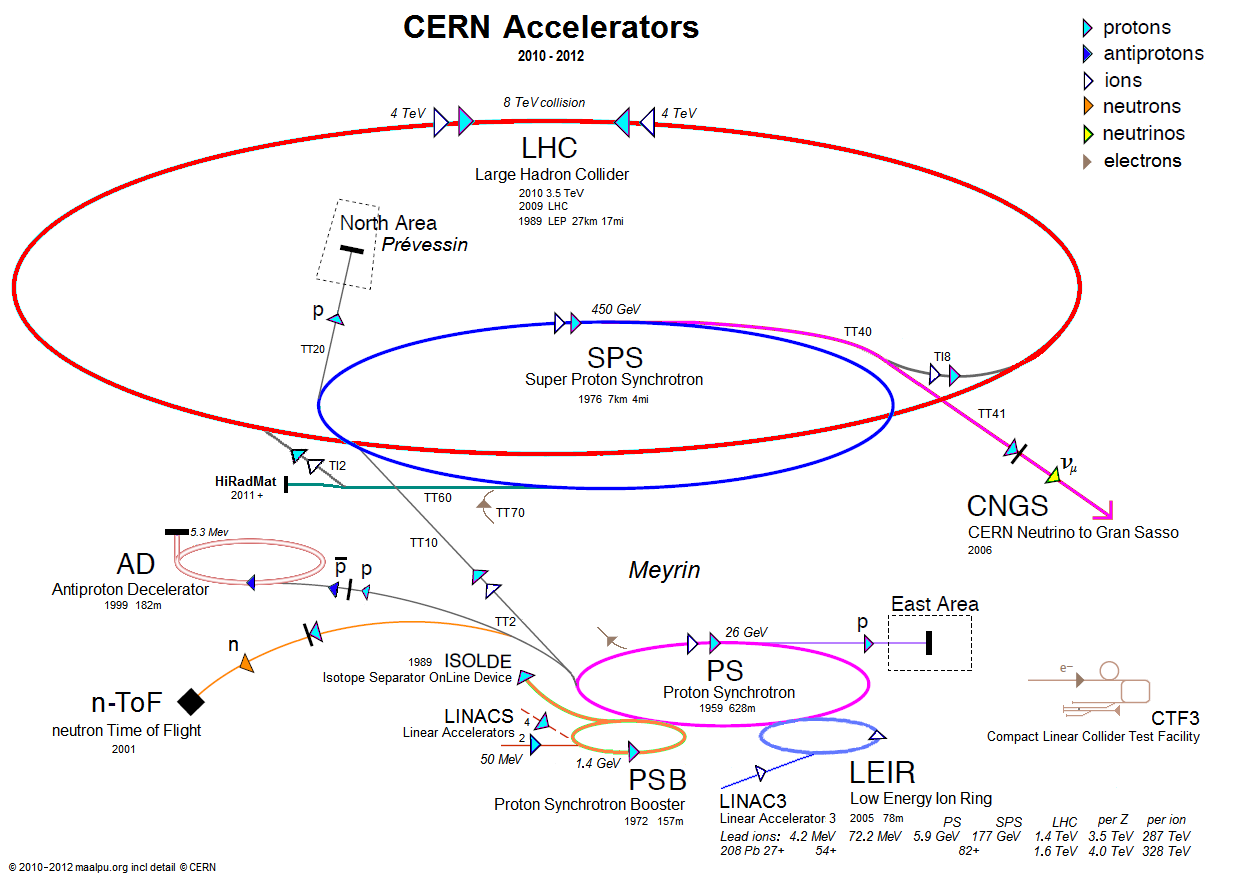
\includegraphics[width=0.90\textwidth]{LHC_chain}
\caption[The LHC accelerator chain.]{The LHC acceleration chain. Protons start in the Linac2 accelerator
(bottom, center), are accelerated through the PSB, PS, and SPS before being
injected into the LHC ring.}
\label{fig:lhcChain}
\end{figure}

The beams are steered using a series of 1232 superconducting dipole magnets, with magnetic
fields of up to 8.3 Tesla. Because there are two proton beams within the LHC ring
circulating in opposite directions, the dipoles have a twin-bore design. In this
setup, there are two beam pipes, with each pipe having its own set of coils to
produce the steering field. In addition to the dipoles, there are 400 quadrupole
magnets which focus the proton bunches. 
%It is only near the interaction regions inside of the detectors that the two beams share one beam
%temp more about magnets?

\begin{table}[h]
\centering
\begin{tabular}{|c|c|c|c|}
\hline
    & 2011 & 2012 & Design \\
\hline
Center of mass collision energy (TeV) & 7 & 8 & 14 \\
Peak Inst. Lumi. ($cm^{-2}~s^{-1}$) & 3.54 & 7.67 & 1.0 \\
Peak Colliding Bunches & 1331 & 1380 & 2808 \\
%Protons per bunch & & & $1.15 \cdot 10^{11}$ \\
Maximum pileup & 16.15 & 34.55 & 19.02 \\
Maximum recorded data, single fill & 118.0 \pbinv & 238.9 \pbinv & -\\
\hline
\end{tabular}
\caption[Machine specifications for the LHC.]{Peak Machine Specifications for 2011 and 2012 proton-proton collisions
at the LHC.} 
%source: https://twiki.cern.ch/twiki/bin/view/CMSPublic/LumiPublicResults#Proton_proton_reference_run_for
%source: https://edms.cern.ch/file/445830/5/Vol_1_Chapter_2.pdf
\label{tab:lhcPerformance}
\end{table}

\begin{figure}[h]
\centering
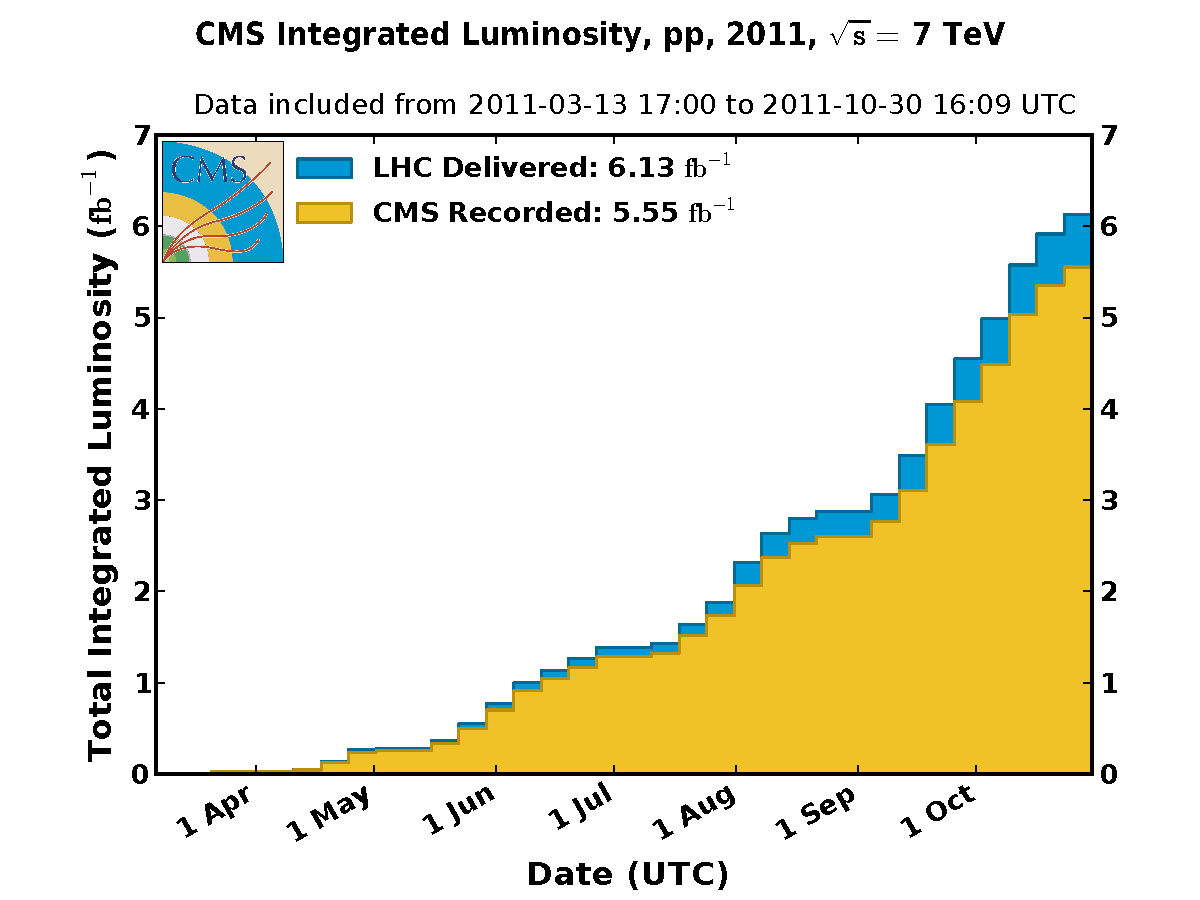
\includegraphics[width=0.45\textwidth]{ppLumi_per_week_2011}
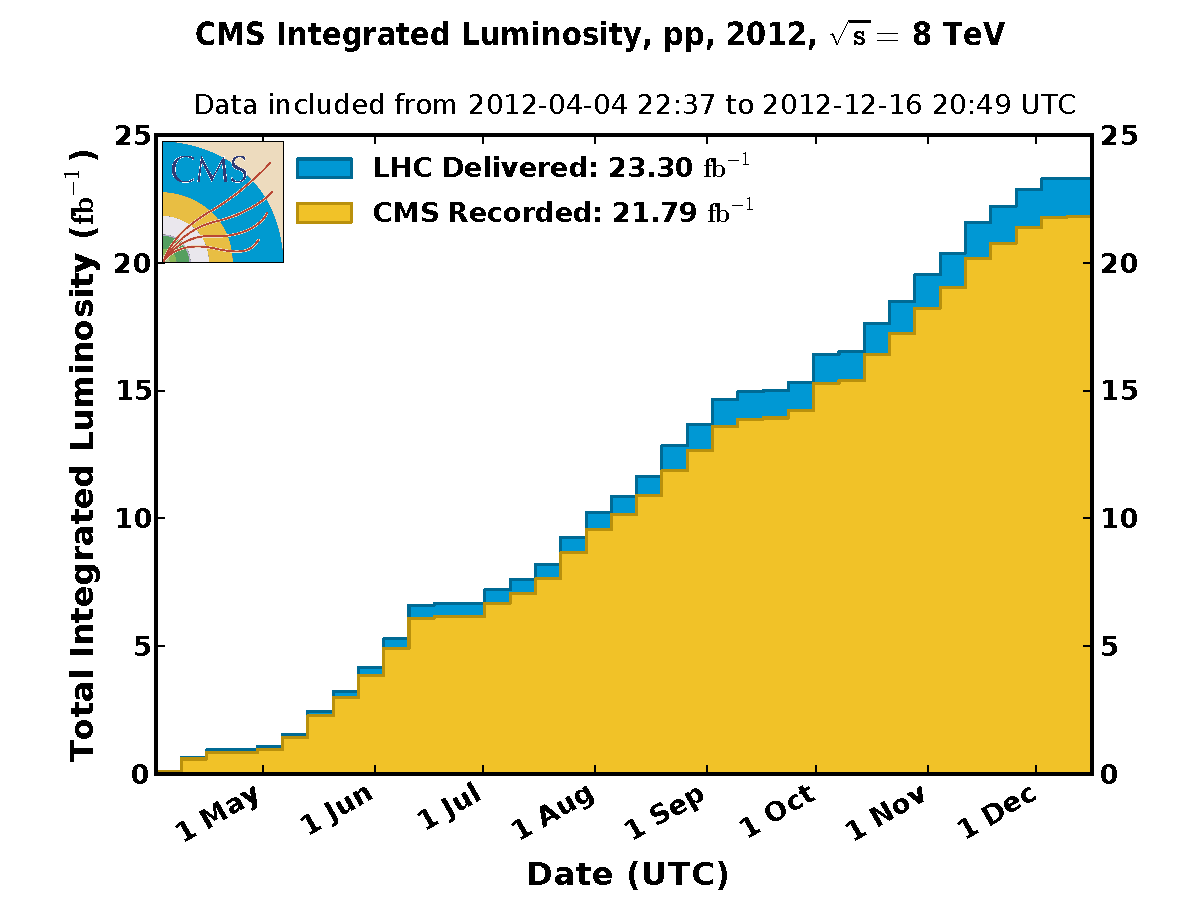
\includegraphics[width=0.45\textwidth]{ppLumi_per_week_2012}
\caption[The amount of intergraled luminosity at the LHC in 2011 and 2012.]{The amount of integrated luminosity delivered by the LHC and recorded
by the CMS detector in each week of 2011 (left) and 2012 (right).}
\label{fig:dataCollected}
\end{figure}

\section{The Compact Muon Solenoid detector}
\label{section:cms}
The Compact Muon Solenoid, or CMS, is one of the two multi-purpose detectors on
the LHC experiment. It is immense, both in size and scope. It is 21.6 meters
long, 14.6~m in diameter, and weighs in at about 12,500~t. The various
components where primarily built on the surface before being lowered into the
detector cavern, 100~m below ground. CMS sits at the LHC ``Point 5,'' located
near the French town of Cessy, roughly on the opposite side of the ring from
ATLAS and the main CERN campus. 

Like many detectors, CMS features an inner tracking system (for determining the
momenta of charged particles), a magnetic solenoid (in order to bend the
trajectory of charged leptons for accurate momenta measurements),
electromagnetic and hadronic calorimeters (for measurements of particle energy),
an outer muon system (for detection of muons, which tend to pass through the
inner components without significant interaction). CMS is unique in the
placement of the magnet outside of the calorimetric elements: the
`compact'-edness of the tracker and calorimeter allow these components to fit
inside the magnet. In traditional detectors, the magnet is placed immediately
outside of the tracking system, meaning that particles can interact (and lose
energy) in the material of the magnet before reaching the calorimeters.

An isometric diagram of the detector is shown in figure~\ref{fig:cmsExploded},
while a cutaway showing a fraction of the xy-plane of the detector with a
simulated collision interaction is shown in figure~\ref{fig:cmsCutaway}

\begin{figure}[h]
\centering
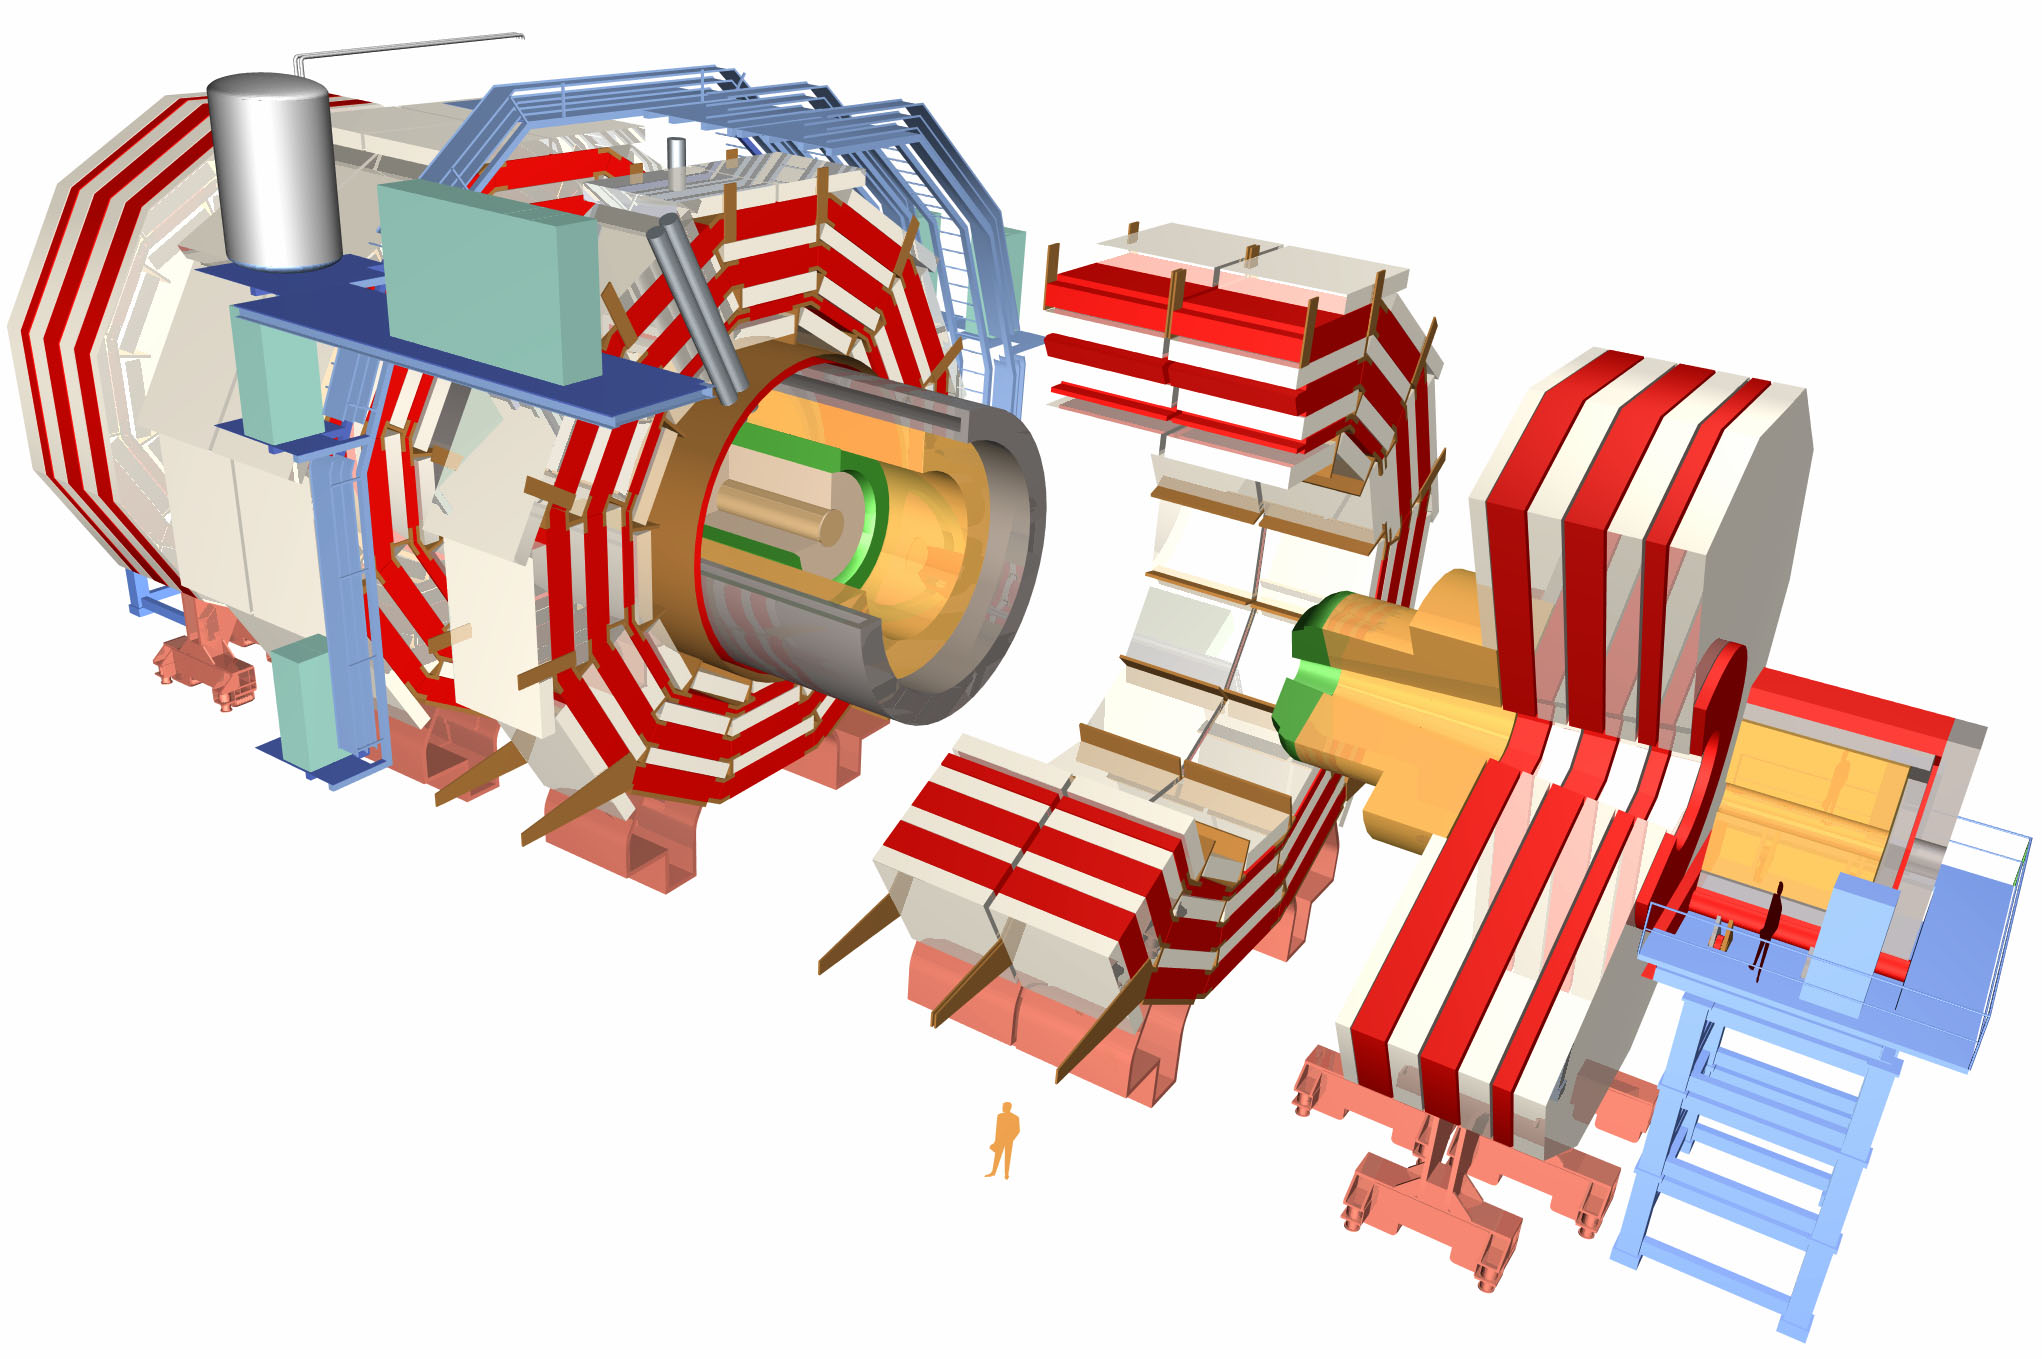
\includegraphics[width=0.6\textwidth]{cms_exploded}
\caption[Isometric view of CMS]{An exploded isometric view of the CMS detector, showing the overall
geometry and layering of the components.}
\label{fig:cmsExploded}
\end{figure}

\begin{figure}[h]
\centering
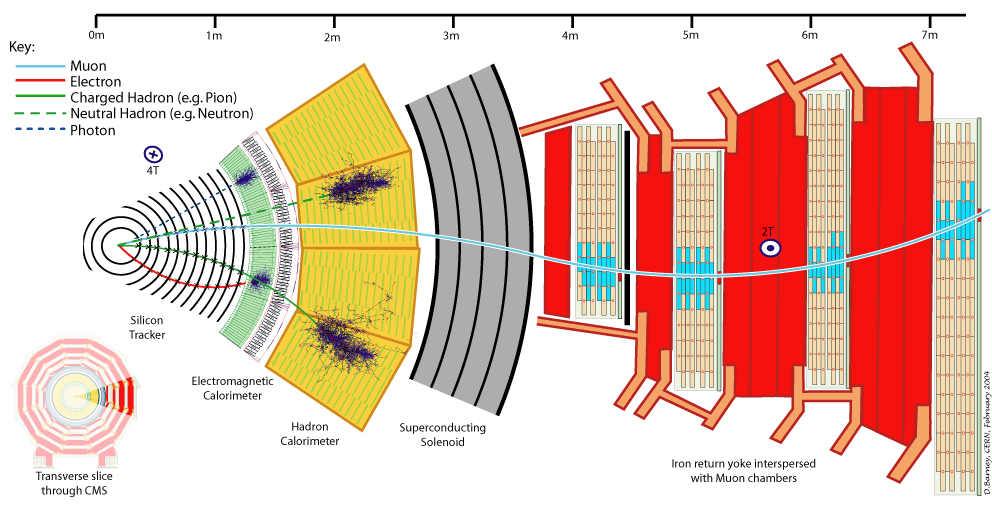
\includegraphics[width=0.8\textwidth]{cms_cutaway}
\caption[A cutaway slice of the CMS detector.]{A diagrammed slice of the CMS detector, showing the components' nesting
and the interactions of different particle types with the subcomponents.}
\label{fig:cmsCutaway}
\end{figure}

\subsection{Tracker}
The innermost component of the CMS detector is the silicon tracking system. Its
role in particle detection is twofold: to provide accurate spatial measurements
for primary and secondary vertices and to accurately measure the curved
trajectories from the charged particles. The tracker system sits just outside
the beampipe, with detecting area starting at a radius of 4.4~cm, extending to
radial distance of 1.1~meters. The system is 5.8~m in length, with disks at
either end of the cylinder to provide coverage in the pseudorapidity range
$|\eta|<2.5$.  The system is made of two subcomponents: the \emph{pixel
detector} and the \emph{silicon strip detector}. In both systems, the primary
technology used for particle detection is reverse-biased np silicon junction. As
charged particles pass through the silicon, ionization deposits in the substrate
cause a depletion current which is read out electronically. The use of this
silicon technology allows very thin sensors to be used, minimizing particles'
interaction with non-detection material while providing the extremely quick
detection response times required by the high collision rates provided by the
LHC. The layout of the tracker is provided in Figure~\ref{fig:trackerLayout}.

\begin{figure}[h]
\centering
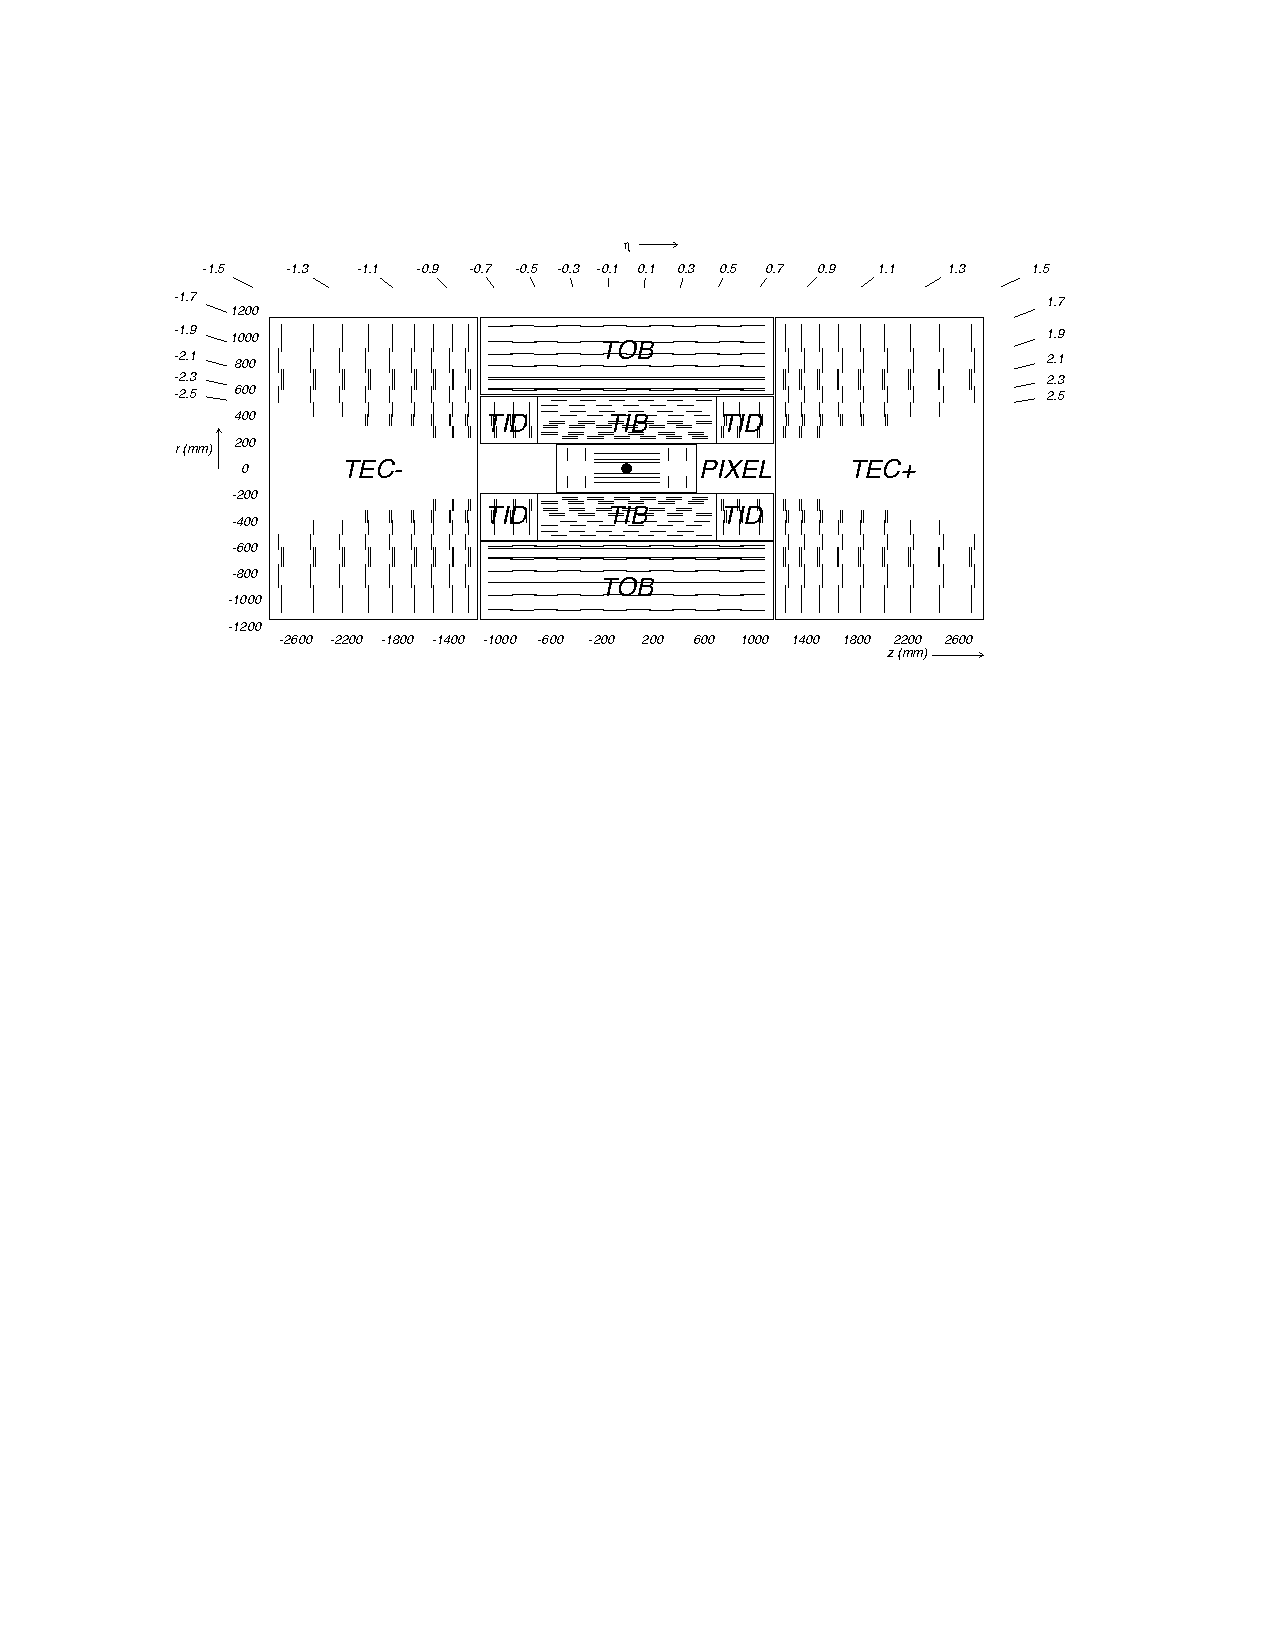
\includegraphics[width=0.8\textwidth]{tracker_layout}
\caption[The geometry of the CMS tracking system.]{The geometry of the inner tracking system of CMS. There are three
central layers of pixel detectors, with an additional two in the forward disk.
There are ten central layers of strip detector, with an additional 3+9 in the
disks.}
\label{fig:trackerLayout}
\end{figure}

The three innermost layers compose the so-called pixel detector,
consisting of 100 $\times$ 150 $\mu m^2$ silicon pixels. These pixels provide
excellent spatial granularity in the most densely occupied region. The primary
purpose of these pixel layers are to provide very fine position measurements in
all three dimensions. The pixels provide measurements in the $r-\phi$ plane with
a resolution on the order of $10 \mu m$ and in the $r-z$ plane to about $20 \mu
m$.  This fine granularity provides the ability to pinpoint, in three
dimensions, the location of primary and secondary vertices. Secondary vertices
are the result of decays of short-lived particles that are born in the primary
interaction (such as a b-quark traveling a short distance before hadronizing
into a jet).  In total, there are 66 million pixels, providing about 1$m^2$ of
detecting area. The position resolution provides CMS with the ability to
accurately locate primary collision vertices, critical both in momenta
measurements of curved tracks and pile-up rejection. Both of these benefits are
discussed in further detail in later chapters of this thesis.

The next 10 layers of the tracking system are covered by the silicon strip
detector, extending to an outer radius of 1.1 m. Because of the lower track
occupancy in this region, the detecting components are not designed to have as
fine a granularity along the $\hat z-$direction.
The strips located in the barrel region  measure $10 cm \times 180 \mu$m in the
inner four layers, known as the tracker inner barrel (TIB), and $25 cm \times
180 \mu $m in the outer six layers (the tracker outer barrel, or \emph{TOB}).
The strip detector subsystem is completed in the more forward endcap regions by
the tracker inner disks (\emph{TID}) and tracker endcaps (\emph{TEC}). 

The information from the pixel and strip detectors are combined to recreate the
path of the charged particles. Because the tracker sits inside of a 3.8~T
magnetic field, the particle paths are curved, allowing measurements of the
momenta through the Lorentz equation:
\begin{equation}
    p = q B R
\end{equation}
where q is the particle's charge, B is the strength of the magnetic field, and R
is the radius of curvature. Particles with higher momenta have as less visible
curvature within the detector and as a result have a larger momenta resolution:
\begin{equation}
    \frac{\sigma(p_T)}{p_T} = p_T \cdot 0.015\% \oplus 0.5\%,  (|\eta|<1.6)
\end{equation}
\begin{equation}
    \frac{\sigma(p_T)}{p_T} = p_T \cdot 0.05\% \oplus 0.5\%,  (1.6 < |\eta| < 2.5)
\end{equation}
The charged particles in this analysis are typically in the 10-50 GeV range,
giving them resolutions on the at the sub-percent level (or a few percent in the
more forward regions).

\subsection{Electromagnetic Calorimeter}
%how does it actually MEASURE energy? IAR 01.May.2013
The next detector component that a particle encounters on its journey outward
through the detector is the electromagnetic calorimeter (\emph{ECAL}). This detector is
designed to capture all of the energy of the electrons and photons produced in
the collisions (or subsequent decays). 

The calorimeter is composed of over 76,000 lead tungstate (PbWO\textsubscript{4})
crystals. As electromagnetic particles pass through these crystals, they produce
electromagnetic showers. The light from these showers is amplified and collected
by avalanche photodiodes in the barrel region and vacuum phototriodes in the
endcap regions. The use of PbWO\textsubscript{4} crystals was motivated by
their radiative resistance, light response, density, and the resulting
compactedness of the calorimeter as a whole.  The dense crystals ($8.28 g/cm^3$)
result in an extremely short radiation length of 0.89$cm$ and a very small
Moliere radius ($2.2 cm$). The geometry of the crystals is designed to utilize
these characteristics, with typical sizes being $22\times22 mm$ at the front
face, $26\times26 mm$ at the rear face, and $230 mm$ in length. As a result,
particles are almost guaranteed to interact somewhere along the crystal length
(traversing roughly 26 radiation lengths), with the resulting EM showers leaking
minimally out of one or two crystals. In addition to the excellent spatial gains of the
crystals, they are additionally very quick. The scintillation decay time is
sufficiently short so that roughly 80\% of the light is emitted within the 25 ns
corresponding to the nominal LHC bunch cross rate. 

The crystals are bundled into submodules, which are grouped into modules which
vary in makeup in order to optimize the uniformity of the crystal coverage.
These modules are then grouped into supermodules, which consist of 1700
crystals, with a 20 crystal coverage in $\phi$ and an 85 crystal coverage in
$\eta$.

The ECAL is composed of of three primary subcomponents: the barrel (\emph{EB}),
the endcap (\emph{EE}), and the preshower (\emph{ES}). The EB covers the area
within $|\eta|<1.479$ and contains the bulk (61,200) of the PbWO\textsubscript{4}
crystals. The EE covers the forward regions, with a pseudorapidity coverage of
$1.56 < |\eta| < 3.0$ and contains 7234 PBWO\textsubscript{4} in each endcap.
The crystals in the endcaps are slightly larger than those in the EB, with a
front face of $28.62\times28.62 mm$ and a rear face of $30 \times 30 mm$ with a
length of 220 mm. The ES sits just in front of the endcap crystals, providing an
$|eta|$ coverage from 1.653 to 2.6. It is composed of
a layer of lead radiators to produce electromagnetic showers, with silicon strip
detectors behind to measure the deposits. The purpose of the ES is primarily to
detect forward neutral pions, in order to distinguish the neutral mesons from
photons. The layout of the ECAL is pictured in Fig.~\ref{fig:ECAL_geometry}.

\begin{figure}[h]
\centering
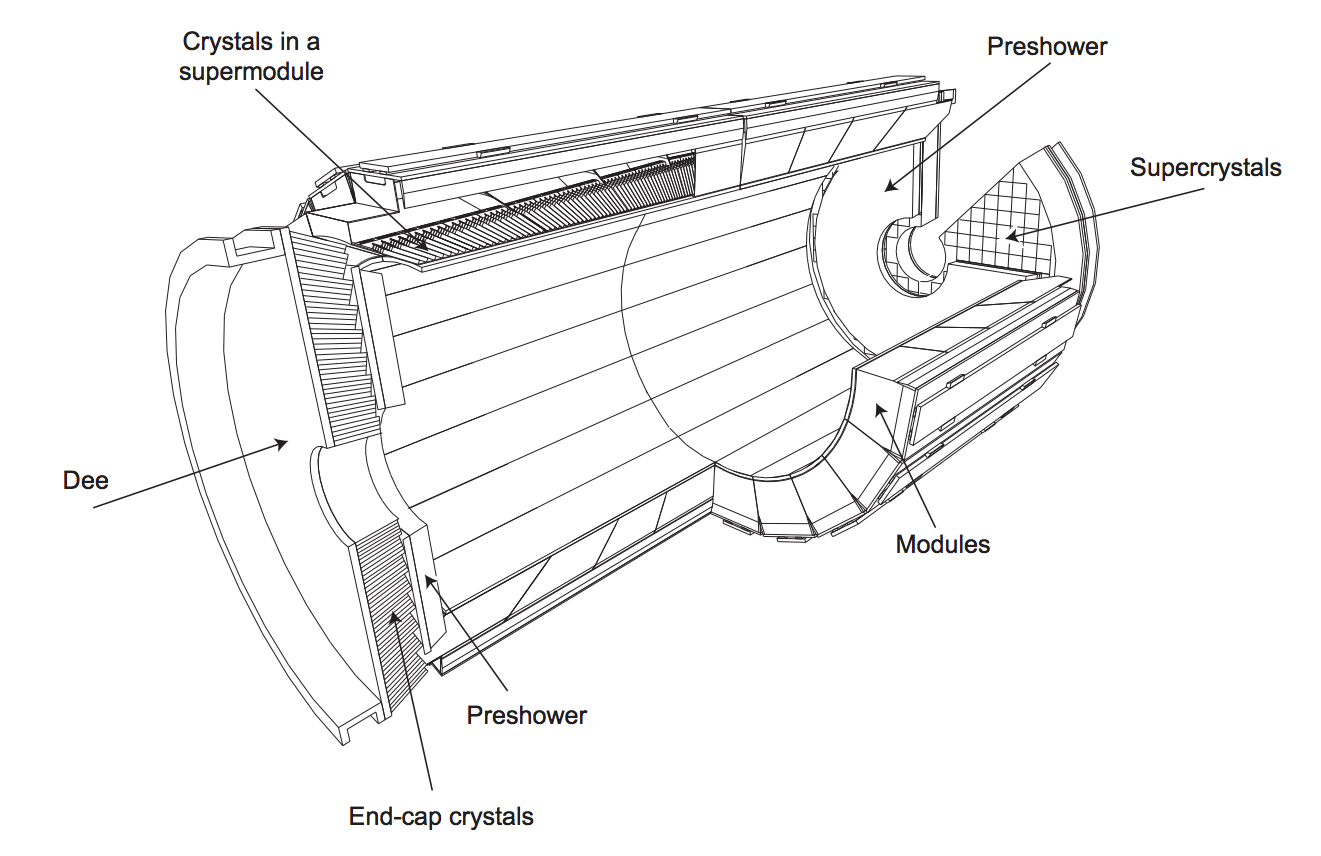
\includegraphics[width=0.8\textwidth]{ECAL_geometry}
\caption[The geometry of the CMS electromagnetic calorimeter.]{The geometry of the CMS Electromagnetic Calorimeter, diagramming the
crystals, modular structure, and overall layout of the EB, EE, and ES
subcomponents.}
\label{fig:ECAL_geometry}
\end{figure}

Because of the high granularity, the ECAL provides excellent spatial resolution
for a calorimeter. However, the crystals' beam-facing orientation combined with
the lack of a segmented depth setup means that there is no information provided
about the angle of the particles as they enter the calorimeter. Thus, the
positional information is limited to the size of the crystals themselves.

The radiation due to the large flux of particles through the detector has the
effect of harming the overall transparency of the crystals. As a result, the
energy measurements tend to drift over time, resulting in systematic deviations
of energy measurements (and larger variations in response from crystal to
crystal).. This is handled using a laser calibration system, which provides a
set of corrections and calibrations which evolve over the length of a run.

The energy measurement of the ECAL is energy-dependent:
\begin{equation}
    \left(\frac{\sigma(E)}{E}\right)^2 =
        \left(\frac{2.8\%}{\sqrt{E}}\right)^2+\left(\frac{0.12}{E}\right)^2+\left(0.30\%\right)^2
\end{equation}
with the energy is provided in~GeV.  The first term is due to the inherent
statistical nature of the EM showering processes, while the second is due to
electronic noise. The third term is due to non-uniformity in the geometric
layout of the detector and calibration uncertainties.

\subsection{Hadronic Calorimeter} 
%still needs more information about the measurements?  IAR 01.May.2013
The Hadronic Calorimeter (or \emph{HCAL}), which sits outside of the ECAL, is
built with the intent to measure the energy of the hadronic jets. It is
important in the measurements of missing transverse energy, which is energy
carried away by non-interacting particles (such as neutrinos or some kinds of
exotic particles). In addition to providing key measurements of hadronic energy,
the HCAL also provides a useful layer of discrimination for potentially fake
electromagnetic particles. If an ECAL deposit is associated with an HCAL
deposit, there is a good chance that the particle was a hadron which interacted
with a nucleus in the ECAL (since truly electromagnetic particles like the
electron will deposit 100\% of their energy in the ECAL).

In addition to its inherent value to jet studies and missing transverse energy
\emph{ME\textsubscript{T}} calculations, the HCAL is also key in measuring the
amount of pileup present in a collision. As most analyses are sensitive to the
number of soft interactions underlying their events of interest, it is important
to account and correct for the energies and compositions of these pileup events.
The HCAL, with its wide coverage in $|\eta|$ provides measurements critical in
these corrections.

The HCAL is a sampling calorimeter, meaning the shower-inducing and energy
measurement components are physically separate media. Like the ECAL, it is split
into barrel and endcap regions (commonly called the HB and HE subcomponents). In
addition, there is a forward hadronic calorimeter (HF), which sits 11~m forward
of the interaction point. Radially, the HCAL fits snugly between the ECAL and
the solenoid, extending from a radius of 1.77~m to 2.95~m. The HB coverage
extends to $|\eta| < 1.305$, while the HE covers $1.305 < \eta < 3.0$. The HF
covers the most forward regions of the detector, covering $3.0 < \eta < 5.0$.
The geometry of the hadronic calorimeter is diagrammed in
figure~\ref{fig:HCAL_geometry}.

\begin{figure}[h]
\centering
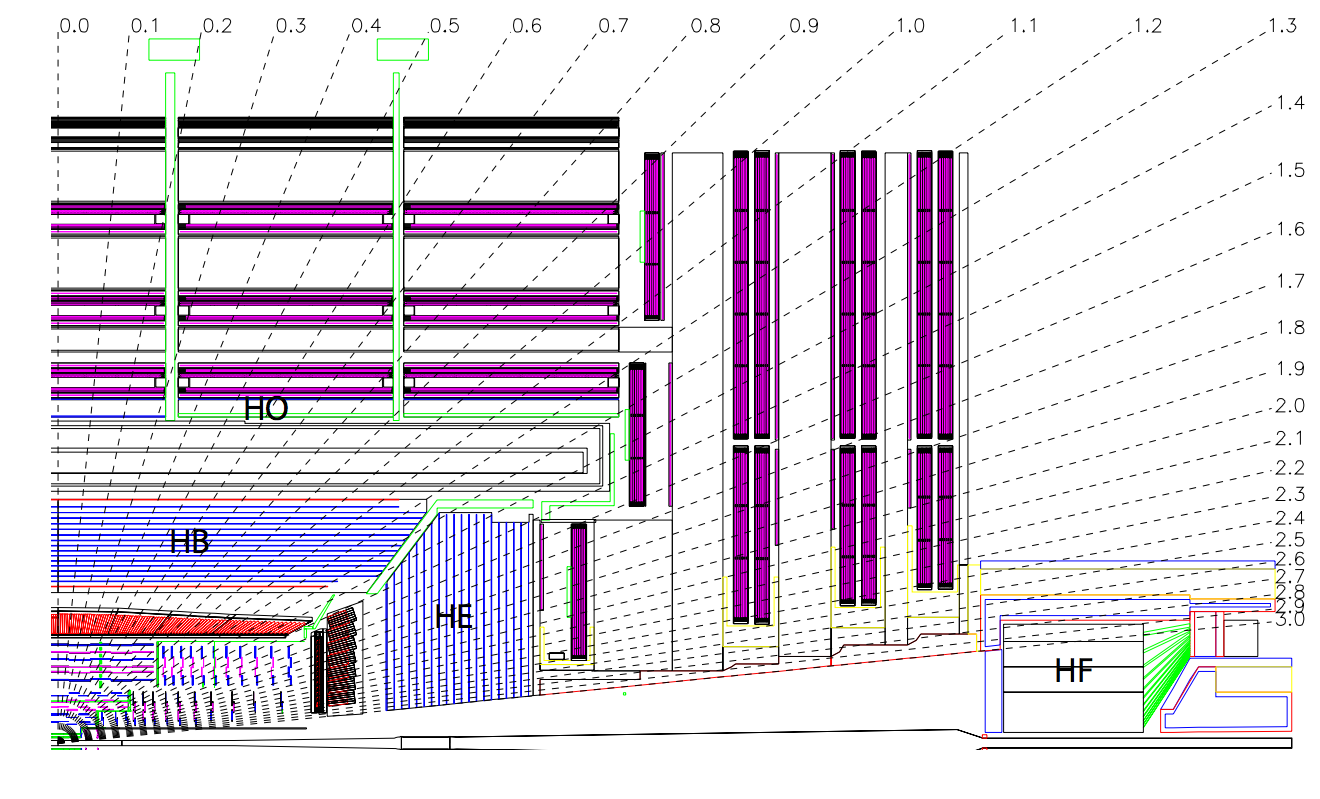
\includegraphics[width=0.8\textwidth]{HCAL_geometry}
\caption[The geometry of the CMS hadronic calorimeter.]{The geometry of a
fraction of the CMS hadronic calorimeter. The HB provides coverage
to $|\eta|<1.3$, the HE covers $1.3<|\eta|<3.0$, and the HF covers
$3.0<|\eta|<5.0$. The dashed lines indicate equal intervals in $\eta$.}
\label{fig:HCAL_geometry}
\end{figure}

The HB and HE subcomponents use interspersed sections of brass (to induce
hadronic showering) and scintillator to measure the resulting energy. In the
more forward HF, where the radiation is a much great concern, the sampling is
done using steel plates coupled with quartz fibers. The interaction length,
$\lambda_i$, of the brass material is 16.42~cm, meaning that a hadronic jet will
be reduced to 1/e of its energy for each 16.42~cm of brass it traverses. The
amount of material increases with the azimuthal angle so that the number of
interaction lengths through the entire HCAL increases from 5.82 $\lambda_i$ to
10.6 $\lambda_i$ at an $|\eta|$ of 1.3. The HE has similar coverage, with about
10 $\lambda_i$ of total material.

The energy resolution for the HCAL is given by:
\begin{equation}
    \left(\frac{\sigma(E)}{E}\right)^2 =
    \left(\frac{90\%}{\sqrt{E}}\right)^2+(4.5\%)^2, HB/HE
\end{equation}
\begin{equation}
    \left(\frac{\sigma(E)}{E}\right)^2 =
    \left(\frac{172\%}{\sqrt{E}}\right)^2+(9.0\%)^2, HF
\end{equation}
where the first term is due to the statistical fluctuations of the hadronic
showering and the second term arises from geometric variations and calibration
uncertainties. 

\subsection{The Magnet}
\label{sub:magnet}
The most striking feature of CMS is the object that gives the detector its name:
the solenoid. The magnet is 6~m in diameter, 12.5~m long, and weighs 220 tonnes.
The superconducting solenoid, consists of 4 layers of NbTi coiling, capable of
producing the 18~kA necessary for the desired 3.8 T magnetic field. This
magnetic field is responsible for causing the trajectory of the charged
particles to bend within the tracker, allowing accurate momenta measurements.
An iron yoke is staggered with layers of the muon chambers, providing the
detector with structural support in addition to feeding a 2~T return field. This
return field allows additional curvature for the muon momenta measurements.

\subsection{Muon chambers}
The outermost component of the CMS detector is the muon system. As suggested by
the name, these subsystems are designed to identify and measure muons. In
addition to the spatial accuracy, it is also critical for the muon systems to be
relatively fast, in order to efficiently trigger on muons within a certain bunch
crossing (as described in~\ref{sub:trigger}). Because muons are so much heavier
than electrons, they largely escape the inner detector components (where the
electrons lose their energy through bremsstrahlung radiation). As mentioned
in~\ref{sub:magnet}, the central portions of the muon system sit in the $\sim$
2~T return field of the solenoid. The field strength, combined with the radial
size of the muon system, allow accurate muon momenta measurements across a wide
spread of energies.

The muon system utilizes three different technologies to achieve its goals of
precise and quick muon measurements. Drift tubes (DTs) are precise, but
relatively slow. This makes them ideal for the barrel region ($|\eta|<1.2$), where particle
rate is expected to be lower. The cathode strip chambers (CSCs) are used
in the more forward regions ($0.9 < |\eta| < 2.4$), where the increased particle
rate requires a quicker technology. Finally, the resistive plate chambers
(RPCs) cover out to $|\eta|<1.6$. RPCs are the quickest technology, but provide
coarser position measurements than either the DTs or CSCs. They are used
primarily for triggering and for resolving ambiguously reconstructed tracks from
other chambers. An overview of the muon system geometry is provided in
Figure~\ref{fig:muonGeometry}.


\begin{figure}[h]
\centering
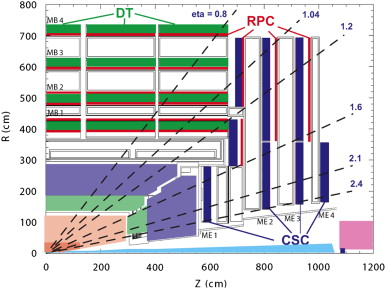
\includegraphics[width=0.6\textwidth]{muon_geometry}
\caption[The geometry of the CMS muon system.]{The geometry of the muon system, composed of the drift tubes (DTs),
cathode strip chambers (CSCs), and resistive plate chambers (RPCs).}
\label{fig:muonGeometry}
\end{figure}

The DT system that covers the barrel area consists of four nested stations. The
inner three systems are composed of 60 drift chambers each, while the outermost
station contains an additional 10 chambers (70 total). The chambers themselves
are filled with a mix of argon and CO\textsubscript{2}. As the muon passes
through the gas, it causes a cascade of ionization. In each cell of the DT
chambers is a long wire under a high voltage. The electrons knocked off of the
gas are pulled to the wires, resulting in a detectable pulse. The time it takes
these electrons to drift to the wire is known as the drift time, and is roughly
380~ns in this gas mixture. The well-known drift time allows for precise
position measurements, but because it is much larger than the 25~ns spacing
between bunch crossings, the drift tube technology can only be applied in the
central area, where occupancy is sufficiently low. The spatial resolution of the
DT system is excellent, providing measurements to an accuracy of 100~$\mu m$ in
the $r-\phi$ plane and 150~$\mu m$ in the $\hat z-$ direction. A schematic of a
drift tube chamber is provided in Figure~\ref{fig:DT}. The half-cell staggering
between cell layers provides the system with a timing resolution of 3.8~ns,
allowing precise identification which bunch-crossing birthed the muon. 

\begin{figure}[h]
\centering
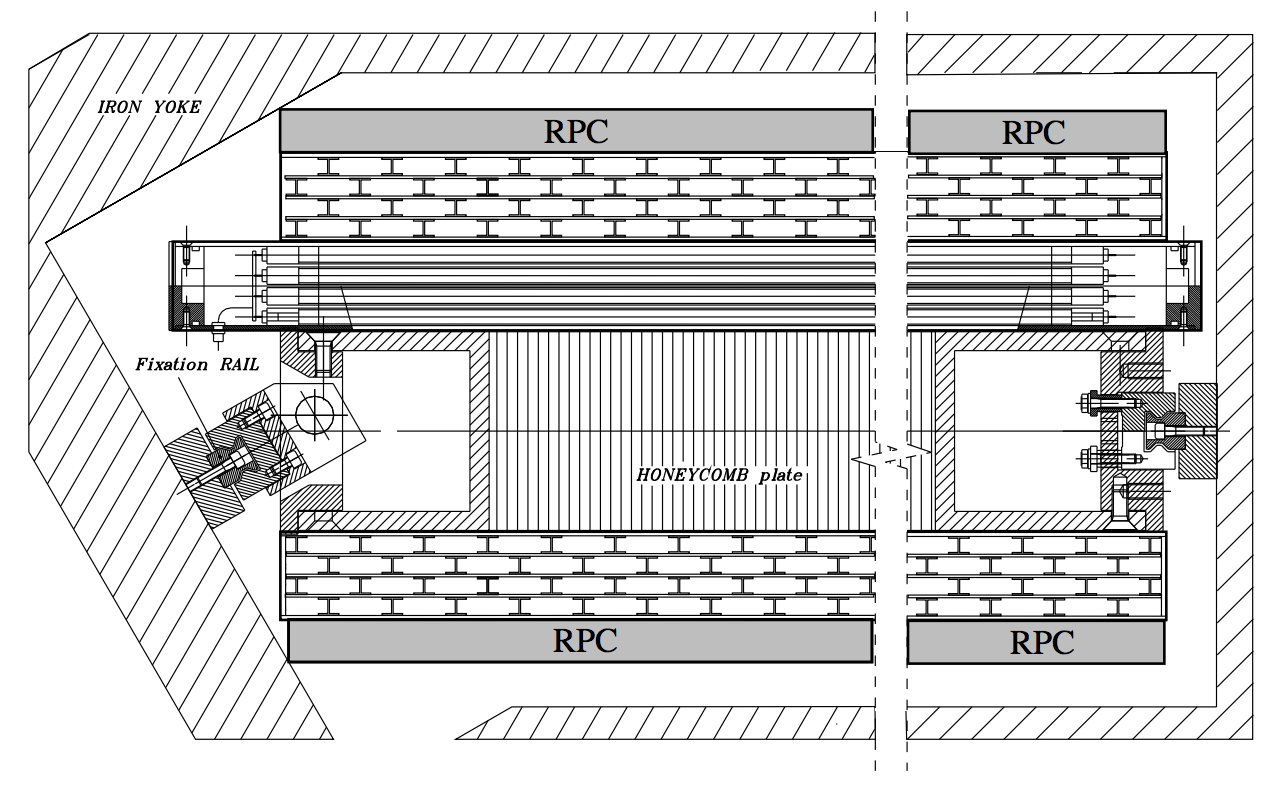
\includegraphics[width=0.8\textwidth]{DT_schematic}
\caption[A schematic drawing of a drift tube chamber.]{A schematic of a drift tube chamber, in the $r-\phi$ plane. Visible are
two cells running parallel to the beamline (immediately above and below the
RPCs) and one cell perpendicular to the beam (above the honeycomb plate).}
\label{fig:DT}
\end{figure}

The CSCs are used in the endcap regions, where the higher flux of particles and 
non-uniformity of the magnetic field make the drift tubes suboptimal. They
consist of a weave of copper cathode strips and anode wires placed within a
volume of gas. Each chamber contains 7 of the cathodes, with 6 planes of wires
running perpendicular across them. The chambers cover 10 or $20^\circ$ of $\phi$
and are staggered in placement to provide full coverage.  Similar to the DTs,
particles moving through the gas result in ionization. The positive ions
produced are pulled toward the negatively charged copper cathodes while the
negatively charged ions are attracted to the positively-charged wires.  As a
result of the fine perpendicular `grid' spacing between the strips and the
wires, the CSCs have a quicker response time than the DTs (CSC pulses last
$\sim 150~ns$, compared to the $\sim 380~ns$ drift time), while maintaining
similar levels of spatial resolution. The overall timing resolution of the CSC
is 7~ns (when utilizing the entire chamber), and its position measurements are
accurate to the 100~$\mu m$ level.

The RPCs are the quickest technology of the muon systems, but provide the
poorest spatial measurements. The chambers consist of two highly resistant
plates separated by a gap filled with gas. An electric field is set up in such a
way that the chambers work in a so-called ``avalanche mode''--when the gas is
ionized by a particle passing through, a cascade of further ionizations occur.
Each RPC detecting element consists of two gaps joined with a common readout
strips between them. The total signal is the combined effect of the two gaps,
providing a higher detection efficiency and lower voltage requirements than a
single-gap setup. Though the spatial resolution of the RPCs is poor in
comparison to the DTs and CSCs (at the 1~cm level), the RPCs have a much
faster response time than the other muon systems, with a time resolution down
to the order of 1~ns. As a result, the RPCs are able to precisely tag which
bunch crossing a given muon came from, making it invaluable in the triggering
process.

\subsection{Data Acquisition and Trigger}
\label{sub:trigger}
The 25 ns design bunch separation means that beam collisions occur with at the
rate of 40~MHz. Because the full detector readout produces on the order of 1 MB
of data per bunch crossing, some 40 TB of potential data is produced in each
second of operation. As it is obviously impossible to store (or readout) such an
enormous amount of data, CMS was designed with a two-stage trigger system to
reduce the rate of stored collisions to a more reasonable (sub-kHz) level. The
filtering must be done in such a way that those events which contain physically
interesting processes are kept, while the uninteresting events are removed. The
Level-1 (L1) trigger is a hardware system that is designed to reduce event rate
to the order of 100 kHz. This subset of the events is then sent to the
High-Level Trigger (HLT), which is a software system implemented on a computing
farm of commercial CPUs. The HLT uses a fuller event reconstruction in order to
make much more involved decisions on the event, resulting in the final filtered
event rate of $\sim 1$~kHz. 

\subsection{L1 Trigger System}
The L1 Trigger system is a hardware system utilizing a mix of FPGAs and 
ASICs. The L1 chain begins locally, where muon chamber track segments or
calorimeter deposits are used to produced Trigger Primitives (TPs).
The TPs are then utilized in a regional calculation, which covers a subsection
of the detector. From the regional stage, a sorted list of objects is passed to
the global trigger subsystems (either the Global Muon Trigger or the Global
Calorimeter Trigger), which determine the highest rank objects from the muon
and calorimeter systems. These are then passed to the Global Trigger (GT), where
there final decision (accept/reject) is made. The accepted events are then
passed to the HLT for further processing. A diagram of the flow through the L1
Trigger system is depicted in Figure~\ref{fig:L1architecture}

\begin{figure}[h]
\centering
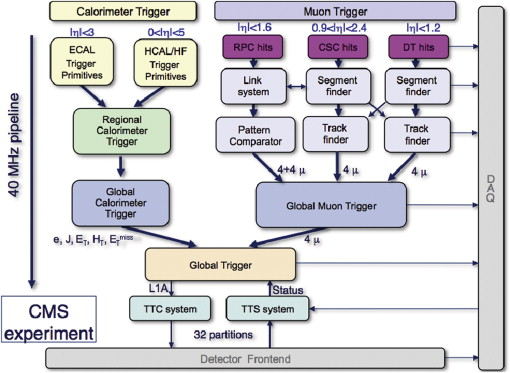
\includegraphics[width=0.7\textwidth]{l1Arch} % source; http://www.sciencedirect.com/science/article/pii/S0168900212009941
\caption[Diagram of the information flow through the CMS trigger system.]{Diagram of the information flow through the CMS trigger system.}
\label{fig:L1architecture}
\end{figure}

\subsubsection{Calorimeter Trigger}
The basic unit in the calorimeter trigger is the trigger tower, corresponding
spatially to a 5$\times$5 grouping of ECAL crystal plus the similarly size HCAL
cell behind it. The energies in each trigger tower are summed by the Trigger
Primitive Generators (TPGs) and passed to the Regional Calorimeter Trigger
(\emph{RCT}) for further processing.  The RCT is made of 18 electronics crates,
each one housing 7 receiver cards and 7 electron identification cards (each of
which provides coverage for two 4$\times$4 regions of trigger towers) and one
jet/summary card. The RCT decompresses the energies reported by the calorimeter
TPGs, and finds the most energetic electron/photon candidates (no distinction
between them is made at this level) within each regions. There are, in addition,
checks to see whether each of these candidates is isolated or not. The RCT
passes the four highest non-isolated candidates, the four highest energy
isolated highest candidates, and the energy sums from each region on to the
Global Calorimeter Trigger (GCT).

As the name suggests, the GCT is the first level at which the calorimeter
information is processed for the entire calorimeter trigger geometry. It uses
this information to compute a number of event-level properties, such as jet
multiplicities, missing transverse energy ($ME_T$), and the scalar jet energy sum
($H_T$). In addition, it finds the highest energy electron/photon candidates
(both isolated and not) and identifies hadronic jets within the calorimeter.
These values are all passed the to GT.

\subsubsection{Muon trigger}
The L1 muon trigger system uses information from all three muon subsystems in
order to maximize the efficiency and background rejection. The CSC and DTs
provide local track segments, which are then combined into regional muon tracks
by their Track Finder systems (CSCTFs and DTTFs). The DT provides coverage in
the barrel region, up to $|\eta| < 1.2$, while the CSCs cover the more forward
regions, $0.9 < |\eta| < 2.4$. The RPC also provide regional
track candidates (with excellent timing resolution) with an $|\eta|$ coverage up
to 1.6. The DT and CSC systems each pass 4 muon candidates to the GMT, while the
RPCs pass a total of 8 (4 from the barrel region and 4 from the endcap region).
Matching between CSC+RPC and DT+RPC candidates ensure that the spatial,
momentum, and timing measurements are optimally efficient for triggering.
This information, consisting primarily of $p_T$, charge, position, and quality
of measurement, is passed to the GT which, in combination with the information
from the GCT, makes a trigger decision based on the event as a whole.

\subsection{HLT System}
After an event is accepted at the L1 level by the GT, it is passed to the
HLT for further processing. Within the HLT, the event goes through 
well-defined reconstruction paths, in order to most quickly comb out those events
which contain potentially interesting physics. Because the event rate coming
through the HLT is still immense (on the order of 100~kHz), the HLT does not
necessarily run a complete event reconstruction--instead it just unpacks and
utilizes the pertinent information, governed by the events' triggers at the L1
level. Because the HLT can utilize more complete snapshots of the event
topology, especially information from the tracker system, it has the ability to
reject a significant subset of events (with fake lepton signals or noisy QCD jet
events), outputting roughly 400~Hz of events for storage.
The triggers utilized in this analysis involve finding two (or more)
isolated leptons above a certain $p_T$ threshold. These are explained in more
detail in Chapter~\ref{chapter:analysis}.

\chapter{Event Generation and Simulation}
\label{chapter:eventGenSim}

In order to guide an analysis (whether the goal is to search for a new particle
or to measure the strength of a physical coupling), it is important to
understand how the physical aspects will manifest themselves within the context
of the LHC and CMS. For optimizing analysis strategies, physicists utilize an
extensive method of simulation, based on the Monte Carlo
methodology~\cite{MCMethod}. From the interactions between quarks, the
kinematics of intermediate particles, the decay into final products, and the
final interaction of final-state particles with the CMS detector, these
simulations are designed to paint a full picture of the physical event.

\section{Monte Carlo Simulation}
\label{sec:mcSim}
The basis of the simulations lies in the Monte Carlo method, which
uses randomization to sample an integration space and, if numerous enough, will
converge to a known underlying distribution. In this way, it is possible to
create enormous samples of simulated events which follow the underlying
equations governing the fundamental interactions. 

The first step in the simulation process is to calculate the \emph{matrix
element} of an process. The matrix element corresponds to the probability of
some physical process, typically visualized with Feynman diagrams like those
from Chapter~\ref{chapter:sm}.  In order to provide a suitably robust set of
simulation events, events are generated by sampling the matrix element
\emph{phase space} (the allowed kinematic regime of a process). For each point
sampled, a weight is calculated, based roughly on how likely an event in that
region of phasespace would be. Once a full sample is produced, the events are
then `unweighted'. In this process, these weights are normalized to
the maximum value. Then, for each event, a random number is thrown and, if the
random number is larger than the normalized weight, the event is rejected. In
this way, the final collection of events each have an equal weight, but are
composed of a properly distributed population.

Because of the complex structure of the collisions at the LHC, it is impossible to
measure (and tune) the momenta of the constituents involved in the processes. As
a result, these matrix elements are also dependent on the \emph{parton
distribution functions} (PDFs). These are probabilistic functions which define
the relative amounts of momentum carried by each of the constituents in the
protons involved in the collision. Due to the energy scales of the interactions
involved, these probabilities are beyond the scope of current QCD calculations,
so as a result, the PDFs are derived based on previous experimental probings of
the partonic structure~\cite{MSTW08,ct10,nnPDF}. A comparison of the three PDF
sets used within this analysis is shown in Figure~\ref{fig:pdfComp}, reproduced
from~\cite{pdfComp}.

\begin{figure}[h]
\centering
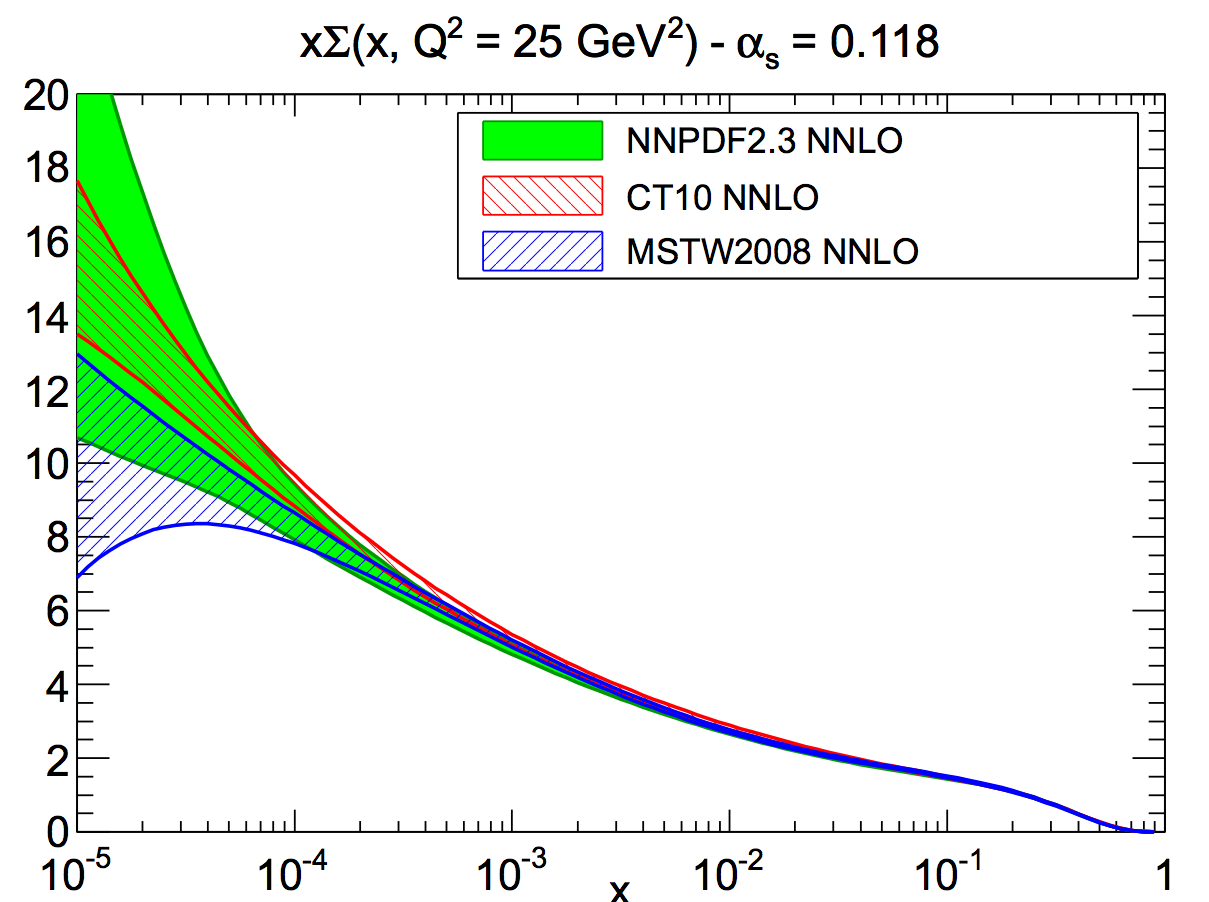
\includegraphics[width=0.80\textwidth]{pdfComp}
\caption[A comparison of three different PDF sets.]{A comparison of the PDF sets NNPDF~\cite{nnPDF}, CT10~\cite{ct10}, and
MSTW08~\cite{MSTW08}, reproduced from~\cite{pdfComp}.}
\label{fig:pdfComp}
\end{figure}

\section{Parton Showering} 
Although the matrix element method outlined in Section~\ref{sec:mcSim} simulates
the hard (high-momentum transfer) of event, it does not provide any simulation
of any of the hadronic showering in the event. As mentioned in
Chapter~\ref{chapter:sm}, individual partons cannot be observed, instead
forming a cascade of hadrons which shower the detector. This hadronic activity
can arise through the hard interactions directly (for example, a \Z boson
decaying hadronically), radiated from an initial or final state, or from the
\emph{underlying event}. The underlying event is a result of QCD's color
conservation--as the partons in the proton interact in the hard process, the
partons that remain in the proton must themselves form into colorless states.

Because of the low energies involved in the soft interactions, it is difficult
(or impossible) to apply the standard tools of QCD calculations to the
hadronization process. Instead, a purely phenomenological approach is taken,
known as the Lund string model~\cite{lundStringModel}. In this model, the partons are
attached with a gluon `string'. As the string stretches (meaning the partons
move apart), its energy increases until it can create new quark/antiquark
pairs, at which point it `snaps'. Quarks and antiquarks from nearby sprays can
combine into mesons, or the quark cascade can continue, as diagrammed in
Fig.~\ref{fig:hadronization}.

\begin{figure}[h]
\centering
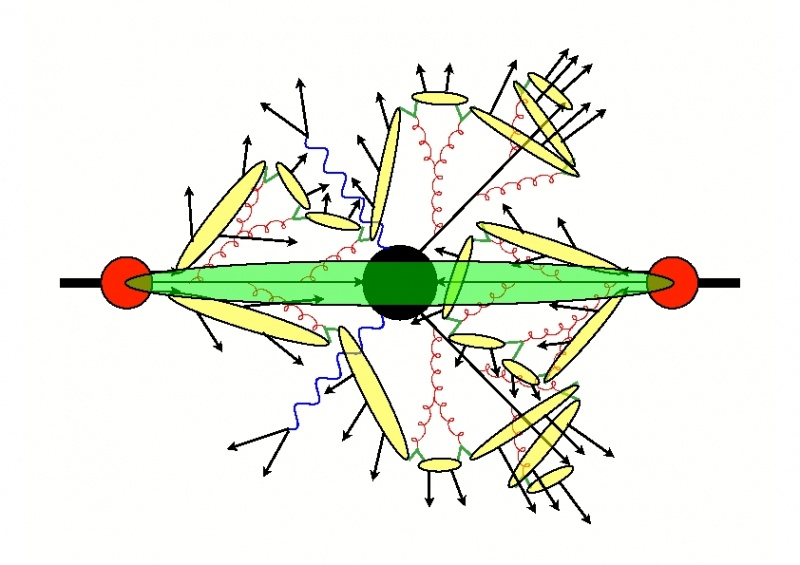
\includegraphics[width=0.80\textwidth]{hadronization}
\caption[Diagrammatic representation of a hadronization process.]{A diagram
depicting the hadronization process\cite{hadronization}. The hard process is
highlighted in green, while the various hadronizations are in yellow.}
\label{fig:hadronization}
\end{figure}

\section{Pile-up}
In addition to the simulation of the hard process and the partonic showering,
simulated physics events also require a description of the \emph{pile-up}.
Pile-up events are interactions which occur between other protons within the
bunch crossing. In order to simulate the effect that these events have on the
hard process, \emph{minimum bias} (soft events) are superimposed on top of the
event of interest. The number of these events added is assigned randomly so that
the overall distribution of the amount of pileup per event matches the data as
closely as possible. Because of the long timeline involved in generating MC
samples, it is necessary to apply corrections in order to properly represent the
distribution in data. These corrections are further explained in
Chapter~\ref{chapter:analysis}).

%\begin{figure}[h]
%\centering
%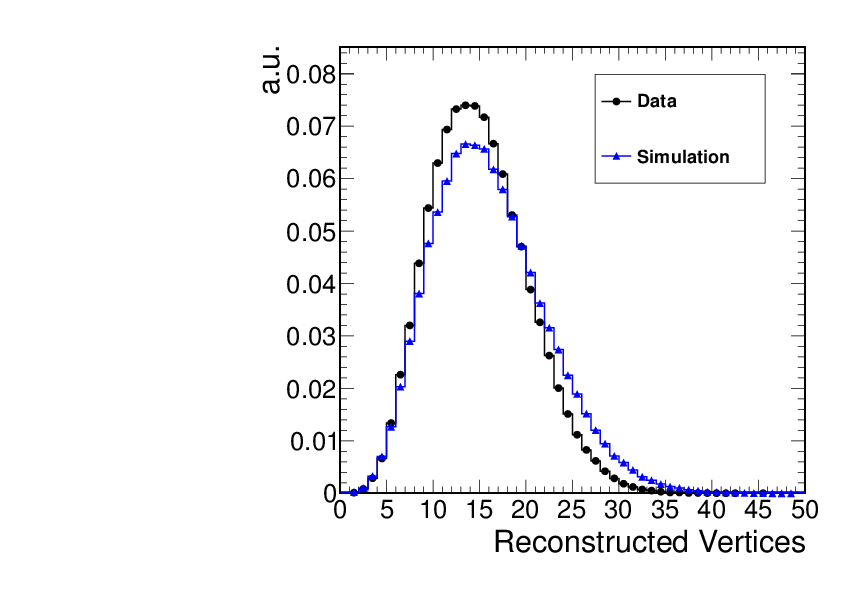
\includegraphics[width=0.80\textwidth]{compvertices}
%\caption[Comparison of data and uncorrected simulated pile-up distributions.]{An example comparison between the simulated number of reconstructed
%vertices (blue triangles) and the final distribution seen in data (black dots).
%The differences are accounted for via corrections explained in
%Chapter~\ref{chapter:analysis}.}
%\label{fig:vertices}
%\end{figure}

\section{Generator Software}

There are many different software packages that have been written for MC event
generation. They primarily differ in the order of the calculation. Some, such as
Sherpa and Pythia, involve only leading order perturbative QCD calculations.
Other generators, such as POWHEG BOX, MADGRAPH, MC@NLO, and MCFM include
next-order effects in the calculations. Typically, the LO MC generators include
the full chain from initial state to final detectable objects. The NLO
generators, are typically interfaced with a second program (commonly PYTHIA) in
order to handle the hadron showering processes.

\section{Samples used}
This analysis utilizes both NLO and LO matrix element generators, while relying
on Pythia~\cite{PYTHIA} for all showering, hadronization, and underlying event
generation.

The primary Higgs boson signal samples are generated using POWHEG~\cite{POWHEG},
covering both the gluon-gluon fusion and vector boson fusion production
mechanisms at NLO. These samples are weighted to NNLO calculations (VBF) or
NNLO+NNLL (gg) (\cite{yellowReport}). Although the generated Higgs $p_T$ spectra
does not match that of the NLO+NNLL calculations, the effects of this difference
were found to be negligible to the analysis as a whole.

Two different matrix element generators are used in production of the Standard
Model ZZ samples. $q\overline q \rightarrow ZZ \rightarrow \ell\ell\ell\ell$
samples are produced with POWHEG at NLO, while $gg\rightarrow ZZ$ production is
handled at LO via gg2zz~\cite{gg2zz}.

Samples with anomalous triple gauge couplings were all produced with
the LO generator SHERPA~\cite{SHERPA}, as it is the only ME generator which has
the requisite couplings modelled. Although only a LO generator, an extensive
study indicated that the generator well reproduces the four-lepton invariant
mass 

MADGRAPH~\cite{MADGRAPH} is used to produce the simulated sample of
$\Z\rightarrow \ell\ell$ plus hadronic jet activity, which is the largest
reducible background. The use of MADGRAPH in these samples is important, as the
accurate modelling of the jets is especially critical, given that this
background enters the signal region through the hadronic jets faking a
signal-like lepton. This sample is weighted to the calculated NNLO cross
section.

More specific information about the samples used in this analysis are in
Tables~\ref{tab:MC_samples}.

\begin{sidewaystable}
\small
\centering
\begin{tabular}{|c|c|c|c|}
\hline

%\multicolumn{4}{|c|}{7 TeV Samples} \\ 
%\hline
%Sample & Generator & $\sigma$ (pb) & Notes\\
%\hline
%
%ZZTo4[l]\_mll4\_7TeV-powheg-pythia6/Fall11& POWHEG & 0.06609 & $m_{\ell\ell} > 4
%GeV$, l=e,mu,tau\\
%ZZTo2[l]2[l']\_mll4\_7TeV-powheg-pythia6/Fall11& POWHEG & 0.152 & $m{\ell\ell} > 4
%GeV$, l, l'=e,mu,tau \\
%GluGluToZZTo4L\_7TeV-gg2zz-pythia6/Fall11& gg2zz & 0.00174 & \\
%GluGluToZZTo2L2L\_7TeV-gg2zz-pythia6/Fall11 & gg2zz & 0.00348 & \\
%DYJetsToLL\_TuneZ2\_M-50\_7TeV-madgraph-tauola & MADGRAPH & 3048 & $m{\ell\ell} >
%4$\\
%
%GluGluToHToZZTo4L\_M-*\_7TeV-powheg-pythia6/Fall11 & POWHEG & * & \\
%VBF\_HToZZTo4L\_M-*\_7TeV-powheg-pythia6/Fall11 & POWHEG & * & \\
%WH\_ZH\_TTH\_HToZZ\_M-*\_7TeV-pythia6/Fall11 & POWHEG & * & \\
%ZZTo4L with aTGCs & SHERPA & 0.046-0.098** & $m_{\ell\ell} > 12 GeV$, e/$\mu$
%only \\
%
%\hline

\hline
\multicolumn{4}{|c|}{8 TeV Samples} \\ 
\hline
Sample & Generator & $\sigma$ (pb) & Fiducial cuts \\
\hline
ZZTo4[l]\_8TeV-powheg-pythia6/Summer12 & POWHEG & 0.07691 & $m_{\ell\ell} > 4
GeV$, l=e,mu,tau \\
ZZTo2[l]2[l']\_8TeV-powheg-pythia6/Summer12 & POWHEG & 0.1767 & $m_{\ell\ell} > 4
GeV$, l, l'=e,mu,tau \\
GluGluToZZTo4L\_8TeV-gg2zz-pythia6/Summer12 & gg2zz & 0.0048 & $m_{\ell\ell} >
4 GeV$\\
GluGluToZZTo2L2L\_TuneZ2star\_8TeV-gg2zz-pythia6/Summer12 & gg2zz & 0.01208 &
$m_{\ell\ell} < 4 GeV$ \\
DYJetsToLL\_M-50\_TuneZ2Star\_8TeV-madgraph-tarball/Summer12 & MADGRAPH &
3503.71 & $m{\ell\ell} > 50 GeV$ \\
DYJetsToLL\_M-10To50filter\_8TeV-madgraph/Summer12 & MADGRAPH & 915 & $10 <
m_{\ell\ell} < 50 GeV$ \\
TTTo2L2Nu2B\_8TeV-powheg-pythia6/Summer12 & POWHEG & 23.64 & \\

GluGluToHToZZTo4L\_M-*\_8TeV-powheg-pythia6/Summer12 & POWHEG & * & \\
VBF\_HToZZTo4L\_M-*\_8TeV-powheg-pythia6/Summer12 & POWHEG & * & \\
WH\_ZH\_TTH\_HToZZ\_M-*\_8TeV-pythia6/Summer12 & POWHEG & * & \\
ZZTo4L with aTGCs & SHERPA & 0.057-0.064** & $m_{\ell\ell} > 12 GeV$, e/$\mu$
only \\

\hline
\end{tabular}
\caption[Summary of Monte Carlo samples used.]{A list of the samples utilized in the 8
TeV portion of this analysis, the generator used, and the sample cross-section.
A * denotes the fact that there was a wide range of Higgs masses used, while a
** means that there was a number of different coupling values used. Full details
for each are explained in Chapter~\ref{chapter:analysis}.}
\label{tab:MC_samples}
\end{sidewaystable}


\section{Detector Simulation}
Once the physics events are generated, their interactions with the material
composing CMS (and their resulting detection) must also be simulated via
GEANT4~\cite{GEANT4}. At its core, this software suite simulates the stochastic
interactions between the particles created in the collision and the matter of
CMS (both detecting and non-detecting). GEANT4 contains an in-depth geometrical
model of CMS, from the specifications of the detecting components to the material
budget of the non-detecting portions (such as structural support and readout
electronics). GEANT4 also provides simulation of the effects of the solenoid,
calculating trajectories based on actual magnetic field measurements. 

GEANT4 provides a picture of how the particles interact with the detector
components, but one final stage remains in the event simulation chain. In order
to be fully comparable to experimental data, the events must pass through a
simulated version of the electronic detector readout. Each subcomponent of the
detector provides an electronics simulation, so that effects of electronic noise
and timing are represented in the simulated samples. At the end of this
simulation chain, the MC samples exist in the same raw format as the data when
read out by the CMS detector. As a result, both simulation and real data can be
passed through the same \emph{reconstruction} process, allowing direct
head-to-head comparisons between the two.

\chapter{Event Reconstruction}
\label{chapter:eventReco}

The data (and the Monte Carlo simulations) come out of the detector (or its
emulated counterpart) in similar collections of raw measurements. At this stage,
only information about tracker hits, muon chamber hits, and calorimeter deposits
exist. In order to be useful in a physics setting, these detector signatures must be
translated into their physics counterparts. The process of running the raw data
through complex algorithms designed to pick out the myriad particles in the
event is called \emph{reconstruction.} A full description of the reconstruction
algorithms utilized in this analysis follows.

\section{Vertex and Track Reconstruction}
The first step in reconstructing the physics content of an event is mapping
hits in the silicon tracker systems to a particle. This is done using a
\emph{Kalman Filter,} which starts at an inner tracking `seed' point and adds
successive hits to each potential track. As it adds hits to the potential
tracks, it propagates a likely position for a next hit forward, giving the
algorithm a place to look for the next contribution. After the track is built,
the process is repeated, building a track from the outermost hits to the inner
regions. This has the effect of smoothing the overall track and minimizing the
measuring errors at the vertex origin~\cite{trackBuilding}. 

Because each event is accompanied by a large number of pile-up events (up to 35
in 2012 running),  it is important to be able to distinguish each particles'
tracks along with where, with respect to the interaction point, they originated
from. These places of origin, known as vertices, are reconstructed in two
phases. First is the \emph{track finding} algorithms, which associate the
measured tracks with a potential vertex. This is done via \emph{deterministic
annealing}, a machine learning algorithm which models the tracks as a
thermodynamic system, clustering the tracks by minimizing the effective free
energy of the system~\cite{detAnnealing, cmsdetAnnealing}. Vertex fitting, on
the other hand, is the process of measuring a vertex's properties (especially
its position and associated errors). Once a vertex is found and fit, the tracks
are again recalculated, using the vertex as an additional position in the track
fit algorithm~\cite{vertexFitting}. In order to separate the vertices associated
with pileup events with the interaction of interest, each event is given a
\emph{primary vertex,} defined to be the one with the highest sum of squared
track transverse momenta.

\section{Electron Reconstruction} 
Electron reconstruction at CMS comprises of combining tracks with matching
\emph{superclusters}, large groups of associated clusters in the ECAL (see
Fig.~\ref{fig:eleReco}). In supercluster construction, the smaller clusters are
collected in such a way as to capture both the primary ECAL deposit and the
deposits spread in $\phi$ that result from bremsstrahlung radiation as the
electron travels its helical course through the detector.

\begin{figure}[h]
\centering
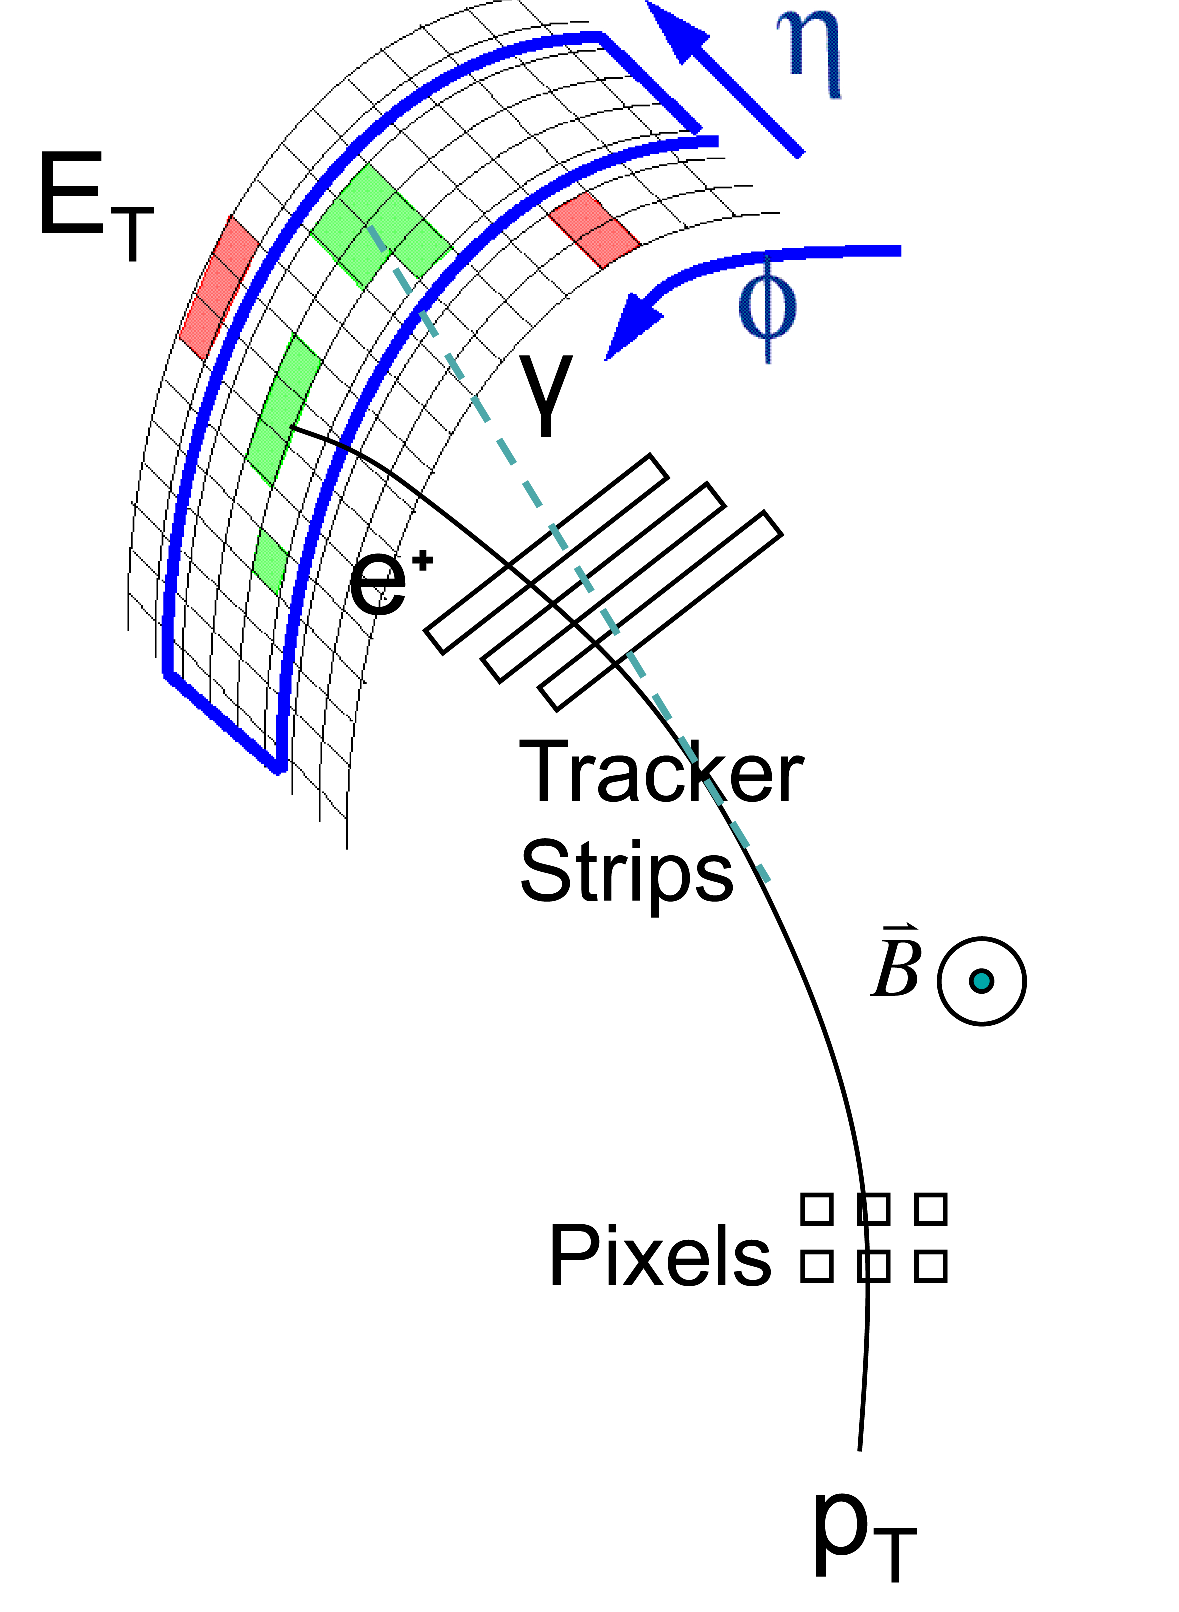
\includegraphics[width=0.40\textwidth]{eleReco}
\caption[Diagram of an electron and its signatures]{Diagram of an electron
travelling through the CMS detector. The electron emits bremsstrahlung radiation
as it bends, resulting in a signature in the ECAL consisting of both the
electron deposit and the radiated photon energies. The supercluster (blue) is a
collection of deposits which capture the electron and associated photon
energies.}
\label{fig:eleReco}
\end{figure}

Basic electron reconstruction can be done in one of two ways. An electron can
either be \emph{tracker-driven} or \emph{ECAL-driven}. The tracker-driven
approach is most effective for electrons that are low in $p_{T}$, starting 
with the collection of reconstructed tracks and searching for compatible hits in
the ECAL. The ECAL-driven approach, on the other hand, is designed to be more
efficient for the higher $p_{T}$ electrons, like those utilized in this
analysis. It begins with the supercluster collection and matches these to hits
in the inner tracker. The full electron trajectories are reproduced using a
Gaussian Sum Filter algorithm. This algorithm allows a more robust reconstruction
of the electron track when compared to the Kalman Filtering, as it is able to
account for the inherent kinks and bends due to the bremsstrahlung processes
the electron can undergo on its journey through the tracker~\cite{gsfElectrons}.

%loose reqs?

In this analysis, additional quality requirements are placed upon the electrons,
as outlined in Chapter~\ref{chapter:analysis}.

\section{Muon Reconstruction}
Muons in CMS are reconstructed using a combination of tracks, independently
reconstructed in the inner tracker and muon systems (colloquially referred to as
tracker tracks and standalone tracks, respectively. Like the electrons, muons
also have two possible modes of reconstruction, depending on whether the
matching begins from the tracker tracks or the standalone tracks.

\emph{Global muon} reconstruction begins in the muon system, taking the
standalone tracks and matching them to tracker tracks that follow a similar
propagation path. The global muon track is then built, using the hit information
in both systems. \emph{Tracker muon} reconstruction begins with tracker tracks
with $p_T > 0.5~GeV$ and total momenta $p > 2.5~GeV$. These tracks are then
treated as potential muons, and their expected paths are extended into the muon
system. If matching segments are found near to the extrapolated muon path, the
matching muon hits are added to the track hits in order to create the muon
object.

Although the inner tracker has greater resolving power in making track momenta
measurements, the muon system provides invaluable information for high $p_T$ ($\sim
100$ GeV) muons. Because these muons bend only slightly while traveling through
the tracker system, the additional hits in the muon system help to resolve the
momenta of these objects.

It is possible for tracks to be reconstructed in multiple muon candidates, as
more than one inner tracks can be geometrically close to the
backwards-extrapolated standalone tracks. These so-called `ghost' muons result
in a non-physical doubling of muon candidates. In order to treat this effect,
which becomes more pronounced in higher pile-up scenarios, the ghost muon pairs
are arbitrated. If two muons are nearby and share more than half of their
segments, the worse of the pair is discarded (as defined by a suite of
criteria based on the track quality measurements and, if needed, additional
identification criteria).

\section{Particle Flow}
Unique in CMS is the so-called \emph{particle flow} process, a suite of
reconstruction algorithms designed to fully reconstruct and identify all the
stable particles created in an event. More specifically, the algorithms are
designed to pick out all of the individual electrons, muons, charged hadrons,
neutral hadrons, and photons in an event. This information can be used in a
number of different ways, from using the identified objects themselves to
recombining the information into jets. Especially relevant to this analysis is
the particle flow muon criteria (which help to establish the collection of
well-identified muons used in the analysis) and the photon, charged hadron, and
neutral hadron collections, which are used to establish how much additional
energy is present near the candidate leptons.

Particle flow first lumps tracks, clusters, and muons into ``blocks,'' which are
simply groups of these objects which pass a loose connectedness test. Individual
particles are then combed out of each block. The process starts with muons,
identifying a particle-flow muon as a global muon with momenta compatible with a
tracker muon. The tracks, muons, and calorimeter signature attributed to the
found muons are then removed from the block and electrons are identified, using
criteria similar to those outline above. Again, associated tracks and
calorimeter clusters are removed from the block. Remaining calorimeter clusters
are assigned to (well-reconstructed) tracks if the deposits are consistent with
a charged-hadron hypothesis, or assigned to neutral hadron or photons, based on
whether the energy was deposited in the HCAL or ECAL. This procedure is
discussed in greater detail in \cite{pflow}.


%\section{Tau Reconstruction}

\chapter{Analysis Strategy}
\label{chapter:analysis}
The ZZ$\rightarrow 4\ell$ analysis is characterized by having four
well-identified, isolated leptons combined into oppositely charged, same flavor
pairs. The selection requirements placed on the leptons are relatively loose
(as described in section~\ref{sec:leptons}), in order to maximize the efficiency
of successfully selecting all four leptons.  Because there are so few physics
signals that result in four prompt leptons, the resulting background
contributions are slight, even with these loose requirements. The primary
reducible background for this signature is a \Z boson produced in association
with two jets. Each jet has a small probability of faking an isolated lepton, as
they can either be tightly collimated (and look like electrons) or can contain a
muon itself which passes selection. This background is estimated from data,
using the methodology outlined in Section~\ref{sec:bgEst}.


\section{Online Selection}
CMS data coming through the data acquisition system is sorted into a number of
\emph{primary datasets}, based on which trigger(s) the event passed. Because the
signature of this analysis is four muons, four electrons, or two muons and two
electrons, the relevant datasets are the DoubleElectron, DoubleMuon, and
Muon+Electron collections. Each of these datasets is used, with overlaps between
them explicitly removed. The trigger menus, which define the L1 and HLT trigger
requirements, evolved throughout the 2011 and 2012 running. At every stage, the
utilized triggers were those with the lowest thresholds which remained
unprescaled (meaning that 100\% of the events passing that trigger were stored).

The online trigger section of the analysis begins with a requirement of finding
two or more leptons at the L1 level, with some loose identification and
isolation criteria applied. These trigger objects are used as input to higher
level triggers, which do further event unpacking and apply a more refined event
selection. The HLT requirements (and their L1 seeds) are summarized in
Table~\ref{tab:triggers}.

\begin{table}[h]
\centering
\begin{tabular}{|c|c|c|}
\hline
Final State & L1 Seed & HLT Trigger \\
\hline
eeee & Two electrons, $E>13,8$ & CaloTrk, $p_T > 17, 8$  \\ %HLT\_Ele17\_CaloTrk\_Ele8\_CaloTrk \\
     & Three electrons, $E>12, 7, 5$ & $p_T > 15, 8, 5$  \\ %HLT\_Ele15\_Ele8\_Ele5\_CaloIdL\_TrkIdVL \\
\hline
$\mu\mu\mu\mu$ & Two muons, one with $E>10$ & $p_T > 17, 8$, * \\ %HLT\_Mu17\_Mu8 \\
               & Two muons, one with $E>10$ & $p_T > 17, 8$, ** \\ %HLT\_Mu17\_TkMu8 \\
\hline
$ee\mu\mu$ & Two electrons, $E>13, 8$& $p_T > 17, 8$ \\ %HLT\_Ele17\_CaloTrk\_Ele8\_CaloTrk \\
            & Two muons, one with $E>10$ & $p_T > 17, 8$ * \\ %HLT\_Mu17\_Mu8 \\
            & Two muons, one with $E>10$ & $p_T > 17, 8$ ** \\ %HLT\_Mu17\_TkMu8 \\
            & One electron $E>12$, one muon & $\mu~p_T > 8, e~p_T > 17$ \\ %HLT\_Mu8\_Ele17\_CaloTrk \\
            & One electron, $E>6$, one muon $E>12$ & $\mu~p_T > 17, e~p_T > 8$ \\ %HLT\_Mu17\_Ele8\_CaloTrk \\
\hline
\end{tabular}
\caption[The L1 seeds and HLT triggers used in each final state.]{The L1 seeds
and HLT triggers used in each final state. A * indicates the presence of two
globally reconstructed muons, while ** indicates the higher $p_T$ muon is
global, while the lower $p_T$ muon is required only at the tracker level.}
\label{tab:triggers}
\end{table}

The numbers in the HLT paths indicate the $p_T$ threshold of the trigger object.
As the triggers do not reach their peak efficiency until a few GeV above the
threshold, in order to not cut into the turn-on curve, offline $p_T$
requirements of 20 and 10~GeV on separate leptons are enforced (as the HLT
requirements on the di-lepton triggers are leptons of 17 and 8~GeV).

Electrons in the di-electron triggers have a set of very loose calorimeter and
tracker based isolations applied, along with a tight calorimeter identification
criteria and very loose track identification. The tri-electron trigger includes
only a loose calorimeter identification criteria on each electron in addition to
a very loose track criteria.

\section{Lepton Definitions}

\label{sec:leptons}
\subsection{Isolation}
A distinct signal of a prompt lepton (one that comes directly from a relevant
physics event) is that it is well-isolated. In general, prompt leptons deposit
recognizable signatures in the tracker and calorimeter subdetectors with little
accompanying energy. Leptons coming from jets (or jets reconstructed partially
as leptons) are often surrounded by additional calorimetric and tracker
activities from the spray of particles that accompany the jet.

In this analysis, the \emph{particle flow isolation} variables are
used~\cite{pflow}. To calculate a lepton's isolation, a cone of size~0.4 in
$\Delta R = \sqrt{\Delta\phi^2+\Delta\eta^2}$ is drawn around each lepton. The scalar sum of the $p_T$ from all the
particle flow objects within this cone are summed up:
\begin{equation}
\label{eqn:PU}
    \textrm{Isolation} = \sum_{\textrm{charged hadrons}} p_T + \sum_{\textrm{neutral
    hadrons}}  p_T + \sum_{\textrm{photons}} p_T
\end{equation}

% vetos

Because isolation is simply a measure of extra energy near a candidate lepton,
it is sensitive to the amount of pile-up present in the event. In order to
correct for this extra energy, two changes are made to equation~\ref{eqn:PU}.
First, only the subset of charged hadrons associated with the primary vertex are
used, removing all the charged hadrons coming from secondary (pile-up) vertices
This is a standard CMS procedure, colloquially referred to as the PFNoPileup
approach. Because the photon and neutral hadron components do not have track
information, they cannot easily be categorized into pile-up and non pile-up
contributions. Instead, pile-up effects are accounted for using the so-called
\emph{$\rho$-correction} (or \emph{fastjet correction}, \cite{fastjet}). In this approach,
the average energy density of all the jet activity in the event is taken as a
measurement of pile-up activity. 
%Jets considered in this measurement are built using the $k_T$ algorithm %cite?
%with 
This number is then multiplied by the
% more precise details on rho?
\emph{effective area} of the lepton, a scaling factor determined by the way the
lepton's neutral hadron/photon isolation component and the event's $\rho$ respond to an
increase in pile-up. These effective areas are taken from independent
measurements from \Z boson production and are provided by the electron and muon
Physics Object Groups. The resulting product, $\rho \textrm{A}_{eff}$ is a
measurement of the neutral hadron+photon isolation contribution due solely to
pile-up events, and is removed from these components.

\begin{equation}
\label{eqn:PU_corr}
\textrm{Isolation} = \sum\limits_{\textrm{charged hadrons}}^{\textrm{non-PU}} p_T + \textrm{max} \left ( \sum_{\textrm{neutral
hadrons}}  p_T + \sum_{\textrm{photons}} p_T - \rho \textrm{A}_{eff}, 0.0 \right )
\end{equation}

The final selection criteria for both electrons and muons is that the amount of
energy near the lepton does not exceed 40\% of the measured $p_T$ of the lepton
itself:

\begin{equation}
\label{eqn:PU_corr}
\left ( \sum\limits_{\textrm{charged hadrons}}^{\textrm{non-PU}} p_T + \textrm{max} \left ( \sum_{\textrm{neutral
hadrons}}  p_T + \sum_{\textrm{photons}} p_T - \rho \textrm{A}_{eff}, 0.0 \right
) \right ) / p_T < 0.40
\end{equation}



\subsection{Impact Parameter Requirements}
A lepton's \emph{impact parameter} can be used help distinguish between prompt
and secondary leptons (which occur due to a photon conversion or a similar
secondary process). The impact parameter is defined to be the distance of closes
approach between the lepton's measured track and the event's primary vertex. In
order to guarantee that all four leptons originate from the primary vertex,
there are loose constraints on the impact parameter:
\begin{equation*}
    d_{Z} < 1.0
\end{equation*}
\begin{equation*}
    d_{XY} < 0.5
\end{equation*}
\begin{equation}
    SIP = \frac{IP}{\sigma_{IP}} < 4.0
\end{equation}
Where $d_{Z}$ is the distance, along the $\hat z$ direction between the impact
parameter and primary vertex, $d_{XY}$ is the distance between them in the
$\hat x \hat y$ plane, and SIP is the separation between the impact parameter
and primary vertex divided by the error in the measurement.


\subsection{Electrons}
\label{sub:eleDef}
Electrons in this analysis begin with the set of reconstructed electrons, as
outlined in chapter~\ref{chapter:eventReco}. They then pass through an identification
process, in order to increase the purity of the electron collection. The
identification is done using a multi-variate analysis (MVA) technique, in which
many electron variables are fed into Boosted Decision Trees\cite{BDTs, BDTs2}.
This process combines information from all of the variables and, based on
training from disparate samples, qualifies the leptons as signal-like or
background-like~\cite{elePerformance, zzHiggsMoriond}.
The variables used in training of the MVA are numerous, but can be split into
three categorizations: electron-track matching, calorimetric signatures, and
track parameters. A list of variables considered in the MVA, along with brief
descriptions of each, are presented in table~\ref{tab:eleVars}.

\clearpage

\begin{sidewaystable}[h]
\centering
\begin{tabular}{|c|p{15cm}|}
    \hline
    \multicolumn{2}{|c|}{Calorimeter-track matching variables} \\
    \hline
    Variable & Description \\
    \hline
    $E_{SC} / p_{in}$ & Total supercluster energy divided by inner track
    momentum \\
    $E_{e}/ p_{out}$ & Energy of cluster nearest to track divided by momenta at
    outermost track position.\\
    $|\eta_{in}|$ & Difference in $\eta$ between the supercluster and the
    closest point of the innermost track extrapolation \\
    $|\phi_{in}|$ & Difference in $\phi$ between the supercluster and the
    closest point of the innermost track extrapolation \\
    $|\eta_{out}|$ & Difference in $\eta$ between the extrapolation from
    the outermost track position and the nearest cluster.\\
    $\frac{1}{E_{tot}} - \frac{1}{p}$ & Reciprocal difference of supercluster
    energy and measured momenta.\\
\hline
\hline
\multicolumn{2}{|c|}{Calorimeter variables} \\
    \hline
    Variable & Description \\
    \hline
    $E_{HCAL}/E_{tot} $ & Fraction of supercluster energy found in HCAL.\\
    $E_{ES}/E_{tot} $ & Fraction of supercluster energy found in preshower.\\
    $\sigma_{i\eta i\eta}$ & Width (in $\eta$) of the primary ECAL cluster.\\
    $\sigma_{i\phi i\phi}$ & Width (in $\phi$) of the primary ECAL cluster.\\
    $\eta$-width & Width (in $\eta$) of the supercluster.\\
    $\phi$-width & Width (in $\eta$) of the supercluster.\\
    $(E_{5x5}-E_{5x1})/E_{5x5}$ & Relative difference between the energy in the
    5x5 and 5x1 pattern of crystals centered on the seed cluster.\\
    R9 & Energy sum in the 3x3 pattern of crystals centered on the seed
    divided by the total supercluster energy.\\
\hline
\hline
\multicolumn{2}{|c|}{Tracker variables} \\
    \hline
    Variable & Description \\
    \hline
    $f_{brem} = (p_{in} - p_{out})/p_{in} $ & Fraction of energy lost, assumed to bremsstrahlung. The
    difference in measured momenta between the innermost and outermost track
    positions.\\
    $\chi^2$ & Chi-squared value of the GSF track fitting.\\
    Hits & Number of measured hits in the Kalman filter track fitting.\\
$\chi^2$ (KF) & Chi-squared value of the Kalman Filter track fitting. \\
\hline

\end{tabular}
\caption[List of electron variables used in the electron idendification MVA.]{List of electron variables used in the electron identification MVA.}
\label{tab:eleVars}
\end{sidewaystable}

\clearpage


The output of the BDT analysis is a number from -1.0 to 1.0, with signal-like
electrons having values closest to 1.0.~\cite{elePerformance}
%An example of the separation is shown in Figure~\ref{fig:eleMVA}, reproduced
%from \cite{eleMVA}.
The training of the MVA and the resulting selection is applied in six separate
electron classifications, split in $p_T$ and $\eta$. In order to pass the
selection, the electron must have an MVA value above the value outlined in
Table~\ref{tab:eleCuts}.

%\begin{figure}[h]
%\centering
%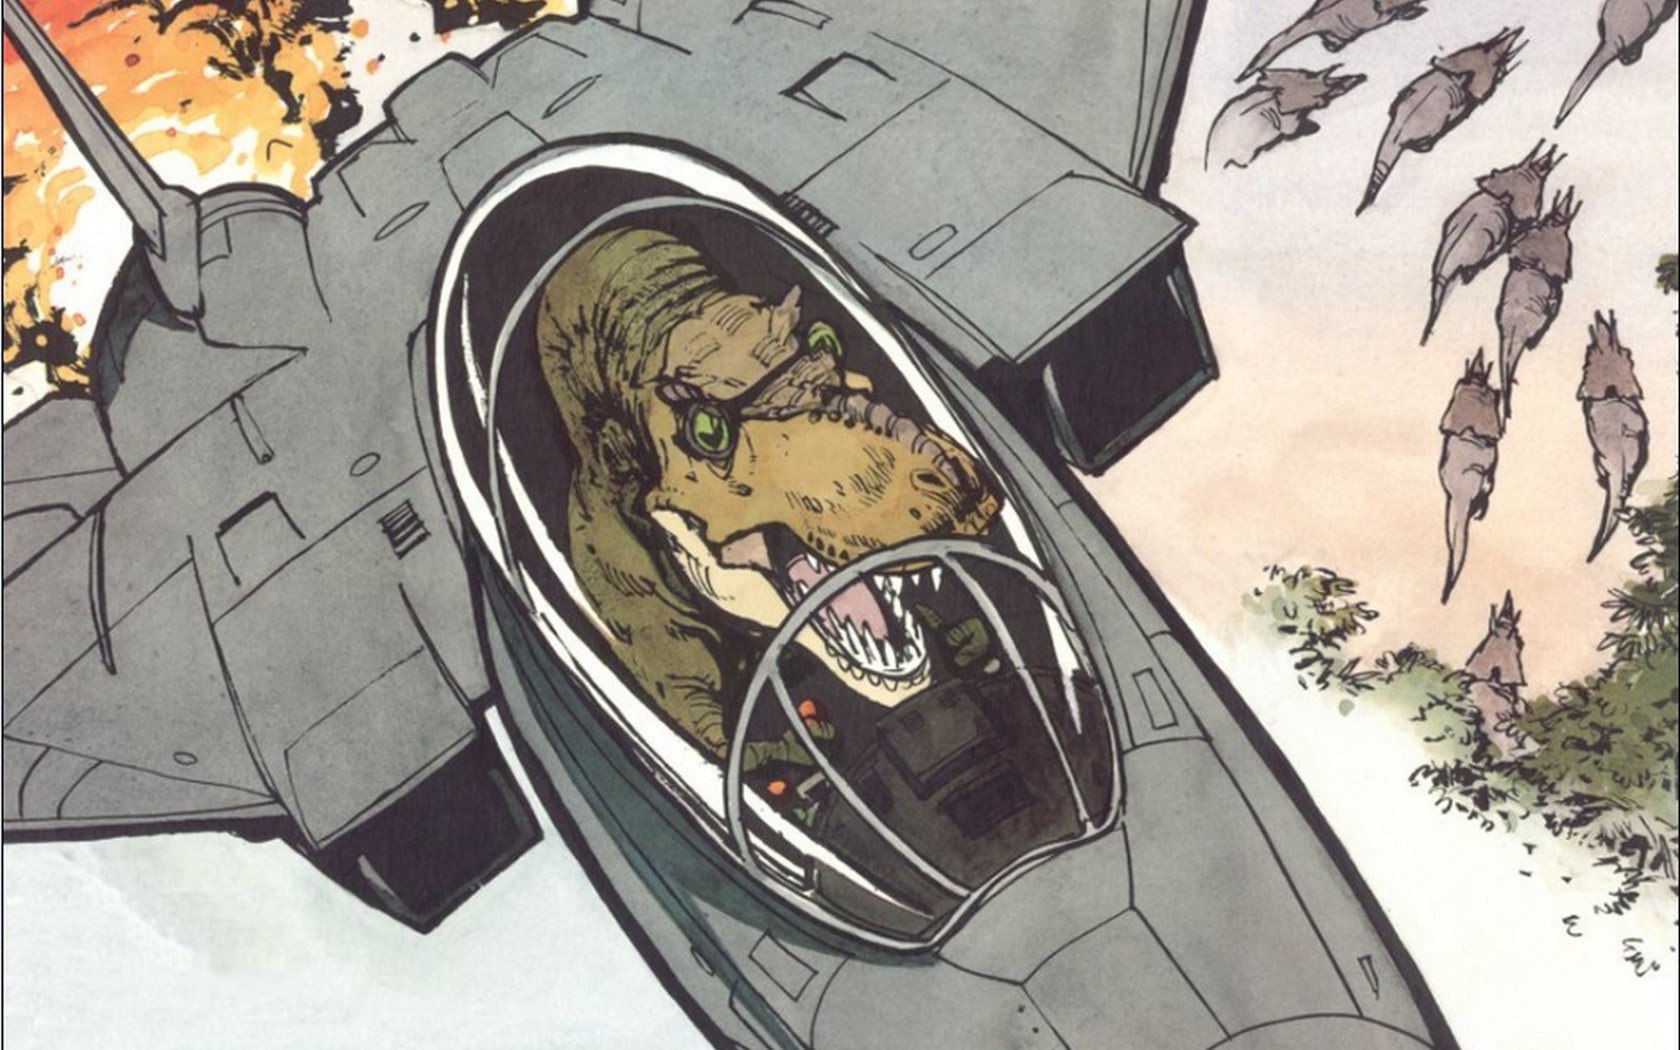
\includegraphics[width=0.80\textwidth]{placeholder}
%\caption[BDT output from the electron identification MVA.]{\temp(stuff), reproduced from\cite{eleMVA}}
%\label{fig:eleMVA}
%\end{figure}

\begin{table}[h]
\centering
\begin{tabular}{|c|c|}
\hline
\multicolumn{2}{|c|}{$5 < p_{T} < 10 GeV$} \\
$0 < |\eta_{SC}| < 0.8 $ & 0.47\\
$0.8 < |\eta_{SC}| < 1.479 $ & 0.004\\
$1.479 < |\eta_{SC}| $& 0.295\\
\hline
\multicolumn{2}{|c|}{$10 GeV < p_{T}$} \\
$0 < |\eta_{SC}| < 0.8 $& 0.5\\
$0.8 < |\eta_{SC}| < 1.479 $& 0.12\\
$1.479 < |\eta_{SC}| $& 0.60\\
\hline
\end{tabular}
\caption[The electron identification criteria.]{The electron identification
criteria. An electron passes the identification stage if the output of its MVA
is greater than the indicated value.}
\label{tab:eleCuts}
\end{table}

The momenta of the electrons is corrected using simulation by applying an
energy smearing technique in order to reproduce the calorimeter resolution
conditions observed in data. Additionally, the energy scale of the electron
superclusters in the data is corrected to match those observed in a Monte Carlo
sample by applying corrections in electrons in $(\eta, R9)$ bins. The
mismeasurement is slight, but time dependent, so the corrections are applied in
a run-range dependent manner.

Additionally, the ECAL energy measurement is corrected using a multivariate
regression technique designed original for the $H\rightarrow \gamma \gamma$
analysis~\cite{HggRegression}. The regression is based on Boosted Decision
Trees, implemented in the TMVA toolset~\cite{BDTs, BDTs2, TMVA}. Training is done using a
Drell-Yan Monte Carlo sample, splitting barrel and endcap electrons into two
separate training categories.  A wide variety of ECAL variables are used in the
process, from shower shape variables and cluster shapes to energy, momenta, and
location measurements.  The regression is designed to correct the simulated
electrons' ECAL energy back to their generated values, from either the raw
supercluster energy (in the barrel) or the supercluster plus preshower energies
(in the endcap). The net effect is an increase in the invariant mass resolution,
especially when one or both electrons are located in the
endcaps~\cite{zzHiggsMoriond}.

All electrons are required to have a fully corrected $p_T >7~GeV$ and to fall
within $|\eta|<2.5$.

\subsection{Muons}
\label{sub:muDef}
The muons utilized in this analysis are selected using a highly efficient set of
criteria, as the risk of fake muons is much lower than that of fake electrons.
As a result, only loose criteria are required to choose real muons while
eliminating a large fraction of the fakes. The muons are required to be
reconstructed via the Global or Tracker reconstruction algorithms (as described
in Chapter~\ref{chapter:eventReco}). In addition, the muons are required to be
identified as muons within the particle flow algorithm\cite{pflow}. Within this algorithm,
a tiered approach to muon identification is taken to ensure that both prompt and
secondary (from a jet) muons are identified with high efficiency. Different
criteria are placed on the muon identification based on whether or not the muon
is isolated or non-isolated. The classification is based on an isolation value
calculated by summing the transverse energy and energy from the tracks and
calorimeter deposits around the muon, within a cone of $\Delta R \le 0.3$. If the
total amount of energy within this cone is less than 10\% of the muon $p_T$, the
loosest criteria are applied to their identification. To be classified as a
PF-muon, there must exist only a valid fit between the tracks in the muon and
inner tracking systems. The muons used in this analysis are expected to be well
isolated, and should in general fall into this category. However, less isolated
prompt muons can still be identified through the so-called PF-loose or PF-tight
criteria. These rely on measurements on the number of muon chamber hits, pattern
matching between tracks and calorimeter deposits, and compatibility between
tracker and muon tracks~\cite{pflowMuons}.

Momentum scale of the muons is calibrated using the \emph{Rochester correction}
method~\cite{rochester}. In this method, corrections are applied to both data
and simulated events, so that the average value of $1/p_{T}$ matches that of a Z
decay as observed by a perfectly aligned CMS. These corrections are applied in
bins of $(Q, \eta, \phi)$, to remove the effects of poorly modeled magnetic
field or incorrect chamber alignments.

Muons are required to have a corrected $p_T >5~GeV$ and to fall within
$|\eta|<2.4$.

\subsection{Scale factors}
\label{sub:scale_factors}
Lepton reconstruction, identification, and isolation efficiencies differ
slightly between data and MC simulation, due to slight inherent differences
between real and simulated detector performance. In order to correct for these
slight differences, the lepton efficiencies are measured in both, compared, and
corrected in the MC samples. The efficiency measurements are done using the
\emph{tag and probe} method. In this method, an independent sample of
Z bosons is selected, by finding opposite sign, same flavor leptons with
invariant mass consistent with that of a  \Z boson. One lepton (called the
\emph{tag}) is required to pass a tight selection criteria, helping to ensure
the purity of the \Z sample. The other leg, called the \emph{probe} is initially
selected using only a loose criteria. This leg is then passed through the
various selection criteria (the identification, isolation, and SIP requirements
especially). After each cut is applied, the candidates are sorted into passing
and failing collections, the Z peak (and the small amount of QCD background) are
fit, and the resulting efficiencies are extracted. The process is done in both
data and Monte Carlo samples, and the ratios (as a function of $p_T$ and
$\eta$ are shown in figure~\ref{fig:tnpResults} (reproduced
from~\cite{zzAN}).  The Monte Carlo simulations are corrected in scale
by applying, for each lepton, the data/MC weight factor for the associated
($p_T, \eta$) bin.  In general, agreement between the simulations and the
observed leptons is excellent, differing only at the percent level. 

The dominant systematic uncertainties on the tag in probe method lie in how the
background and Z peak are modelled. Because the efficiency values
are extracted via a background-subtracted fit, these tails can have a
considerable effect on the final values. A conservative systematic is evaluated
by scaling the number of events in the tails up and down by a factor of two, 
recalculating the efficiency, and taking the difference from the central value
as the systematic uncertainty. Additionally, a 1\% effect is added in quadrature
to account for the shape of the \Z pole. The size of these uncertainties is
summarized in section~\ref{sec:systematics}.

\begin{figure}[h] \centering
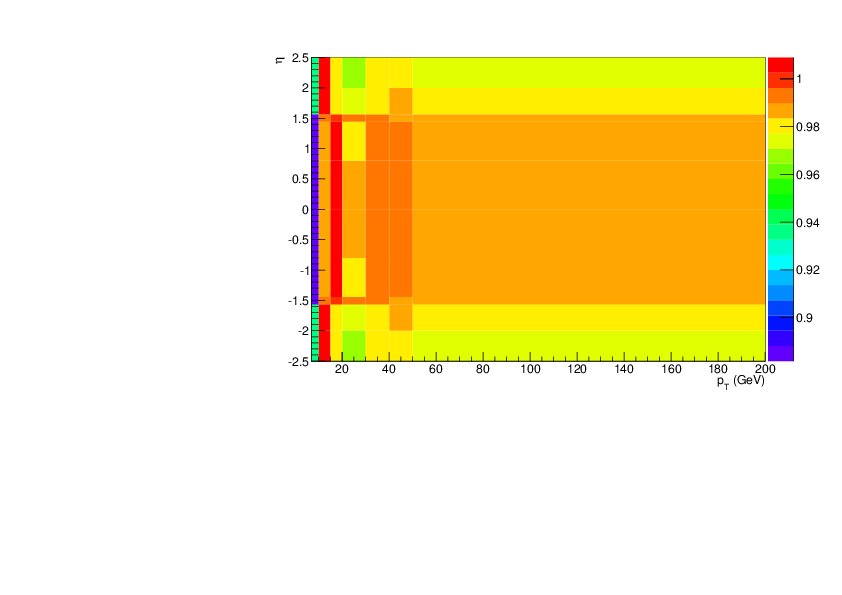
\includegraphics[width=0.60\textwidth]{ele_tnp_corrections} 
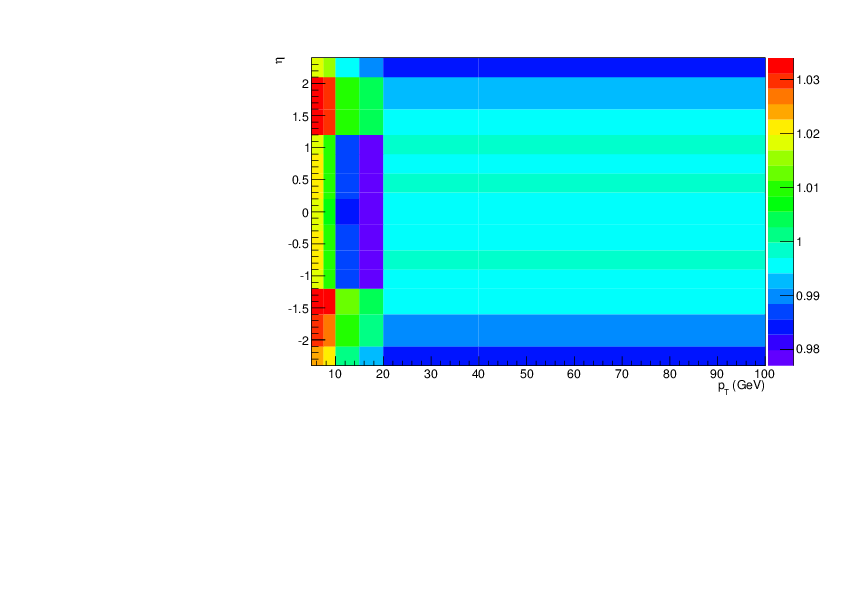
\includegraphics[width=0.60\textwidth]{mu_tnp_corrections}\\
\caption[Ratio of lepton efficiencies between data and monte carlo simulations
for electrons and muons.]{Ratio of lepton efficiencies between data and Monte Carlo simulations
    for electrons (top) and muons (bottom). Results are reproduced
from~\cite{zzAN}.}
\label{fig:tnpResults}
\end{figure}

\section{Pile-up Reweighing}
\label{sub:pileup}
Because the simulated samples were produced with a pile-up scenario
(which does not match the overall scenario in the final data samples), the
simulated samples must be reweighted. By giving the simulated events a slightly
higher or lower weight factor in the final distributions, it is possible to
create a simulated sample whose net pile-up closely resembles that which is
observed in the data.

The distributions of the reconstructed vertices, while a good indicator of pile
up activity, are susceptible to biases coming from the trigger and vertex
finding algorithms. As a result, the ``true'' number of pile-up interactions are
used. In the Monte Carlo simulation, this number is immediately accessible. In
the data, it comes from instantaneous luminosity measurements, stored in
per-bunch-crossing per-luminosity section intervals. This measurement, combined
with the total pp cross-section, is used to determine the pile-up distribution,
as observed by CMS, as it evolves in time. The ratio between the observed and
simulated pile-up distributions for each bin in the simulated distribution tells
how those events must be weighted in order to match the observed.

To test the effectiveness of using the ``true'' pileup variables described, one
can easily check the effect on the reconstructed vertex distribution.  The
results can be seen in figure~\ref{fig:puCorrs}. After corrections, the MC
sample successfully reproduces the pile-up scenario observed in data.
\begin{figure}[h]
\centering
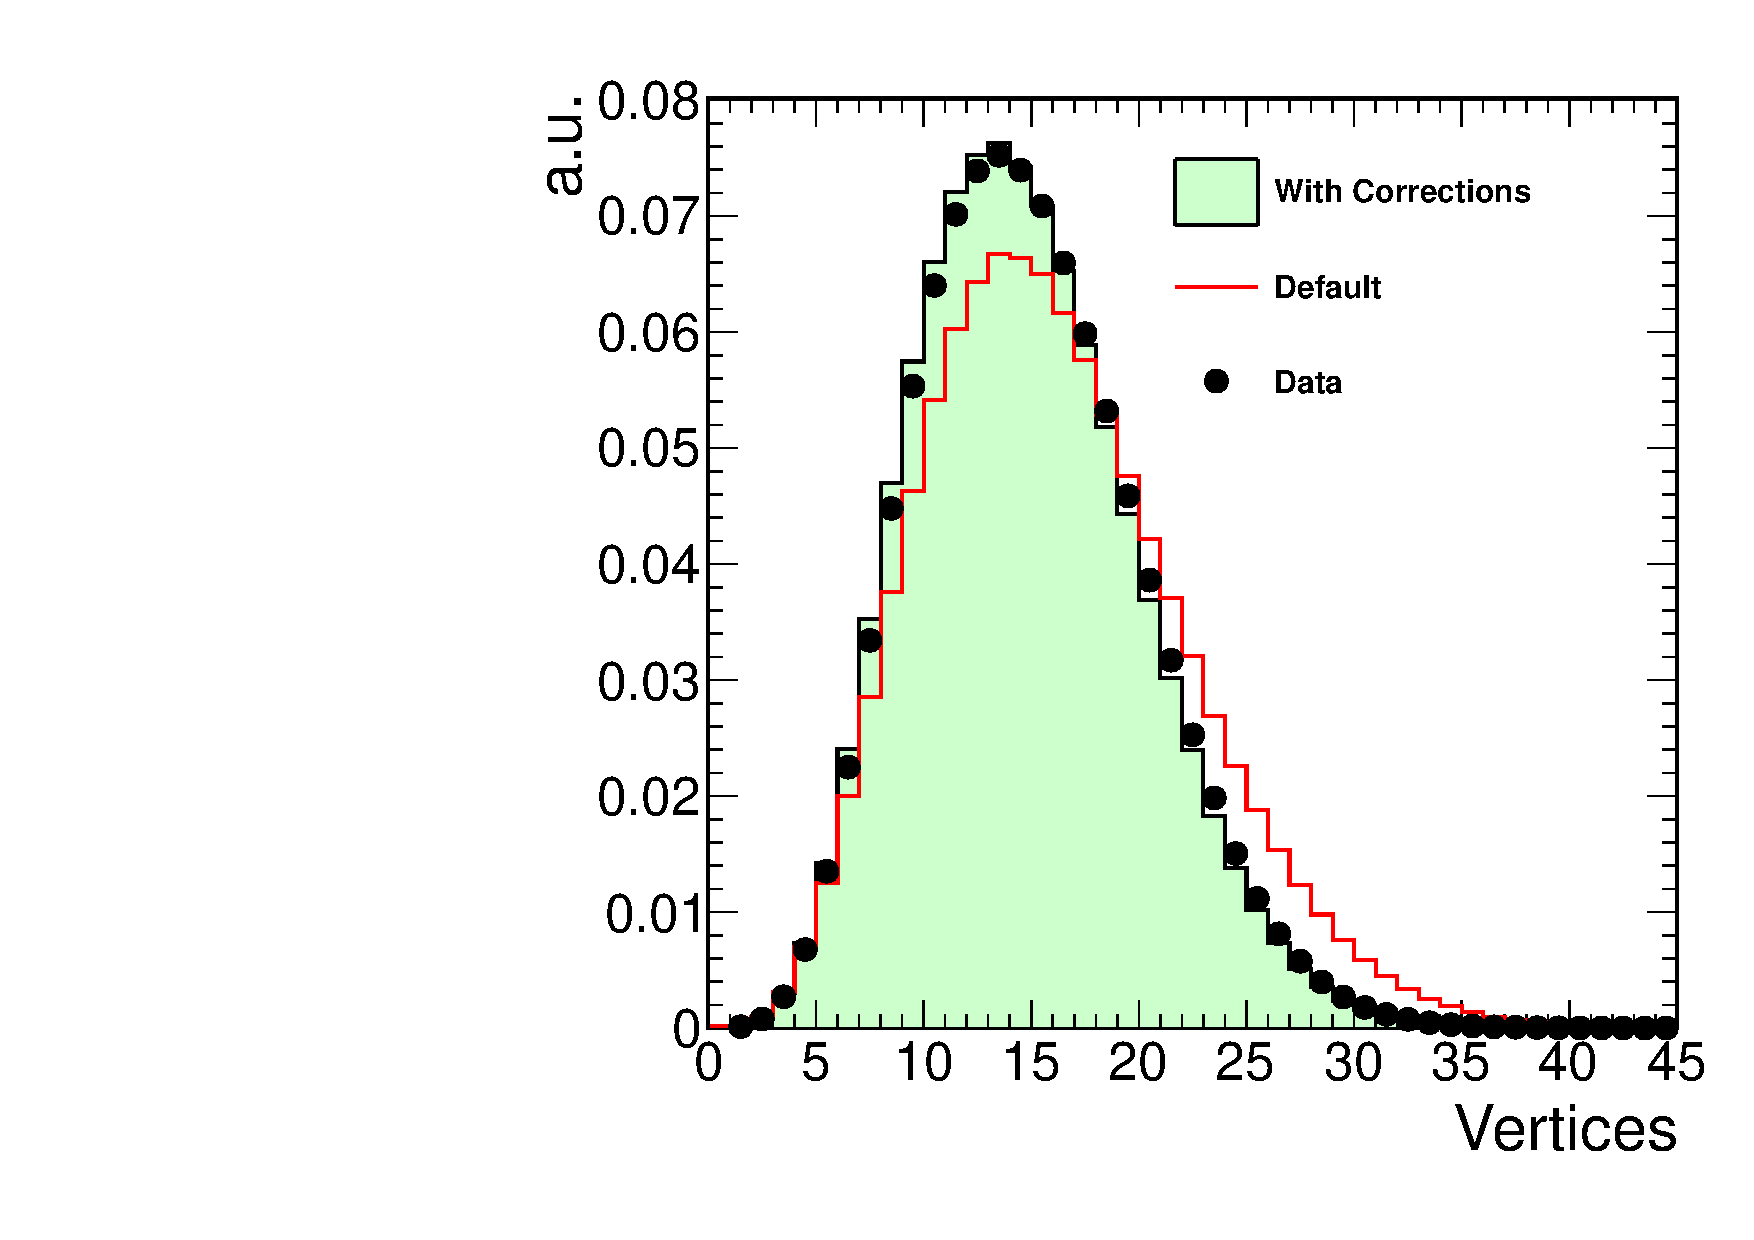
\includegraphics[width=0.80\textwidth]{pu_corrected}
\caption[The effects of pile-up corrections on the rectonstructed vertex
distribtion.]{The effects of pile-up corrections, as described in the text, on
the reconstructed vertex distribution. There is a significant improvement in the
MC-data agreement when the corrections are applied.}
\label{fig:puCorrs}
\end{figure}


\section{Background Estimation}
\label{sec:bgEst}
To estimate the reducible background contribution (coming primarily from a
Z+jets signature with a much smaller contribution from the W/Z+jet production),
a data-driven ``fake-rate method'' is utilized. In this approach, the
probability for a loosely identified lepton (interpreted physically as a jet) to
pass the full lepton selection is calculated. This fake rate is then applied to
the population of a number of subregions which are dominated by these background
physics events. This gives an estimate of the number of these events which are
expected to pass the final selection criteria.

The first step is measuring the leptonic fake rates. This is done using in a
``$\Z + 1 \ell$'' region, where one \Z boson is fully selected and there is exactly
one additional loose lepton found in the event. These leptons have the
requirements from Table~\ref{tab:looseLeps} applied, with an additional
event-level requirement of less than 20~GeV of missing transverse energy (in
order to cut down contamination from WZ production).

\begin{table}[h]
\centering
\begin{tabular}{|c|c|}
\hline
Electrons & $p_{T}>7$~GeV\\
& $|\eta|<2.5$\\
& $<2$ missing inner tracker hits\\
& $|d_{XY}| < 0.5 $~cm  \\
& $|d_{Z}| < 1.0 $~cm \\
\hline
\hline
Muons & $p_{T}>5$~GeV\\
& $|\eta|<2.4$\\
& Global OR Tracker (with $\ge$ 1 segment matched)\\
& $|d_{XY}| < 0.5$~cm  \\
& $|d_{Z}| < 1.0$~cm  \\
\hline
\end{tabular}
\caption[Loose lepton definitions.]{The criteria placed on the loose lepton objects.}
\label{tab:looseLeps}
\end{table}
The leptonic fake rates are then measured as the number of loose leptons which
pass final lepton selection (as defined in sections~\ref{sub:eleDef}
and~\ref{sub:muDef}).
\begin{equation}
    \label{eqn:fr}
    f = \frac{\textrm{Passing full selection}}{\textrm{Passing loose
    criteria}}
\end{equation}

These fake rates, as a function of lepton $p_{T}$, are depicted in
figure~\ref{fig:fakerates}. The dependence on $p_{T}$ is slight, and the fake
rates are applied in a $p_{T}$ independent manner.
\begin{figure}[h]
\centering
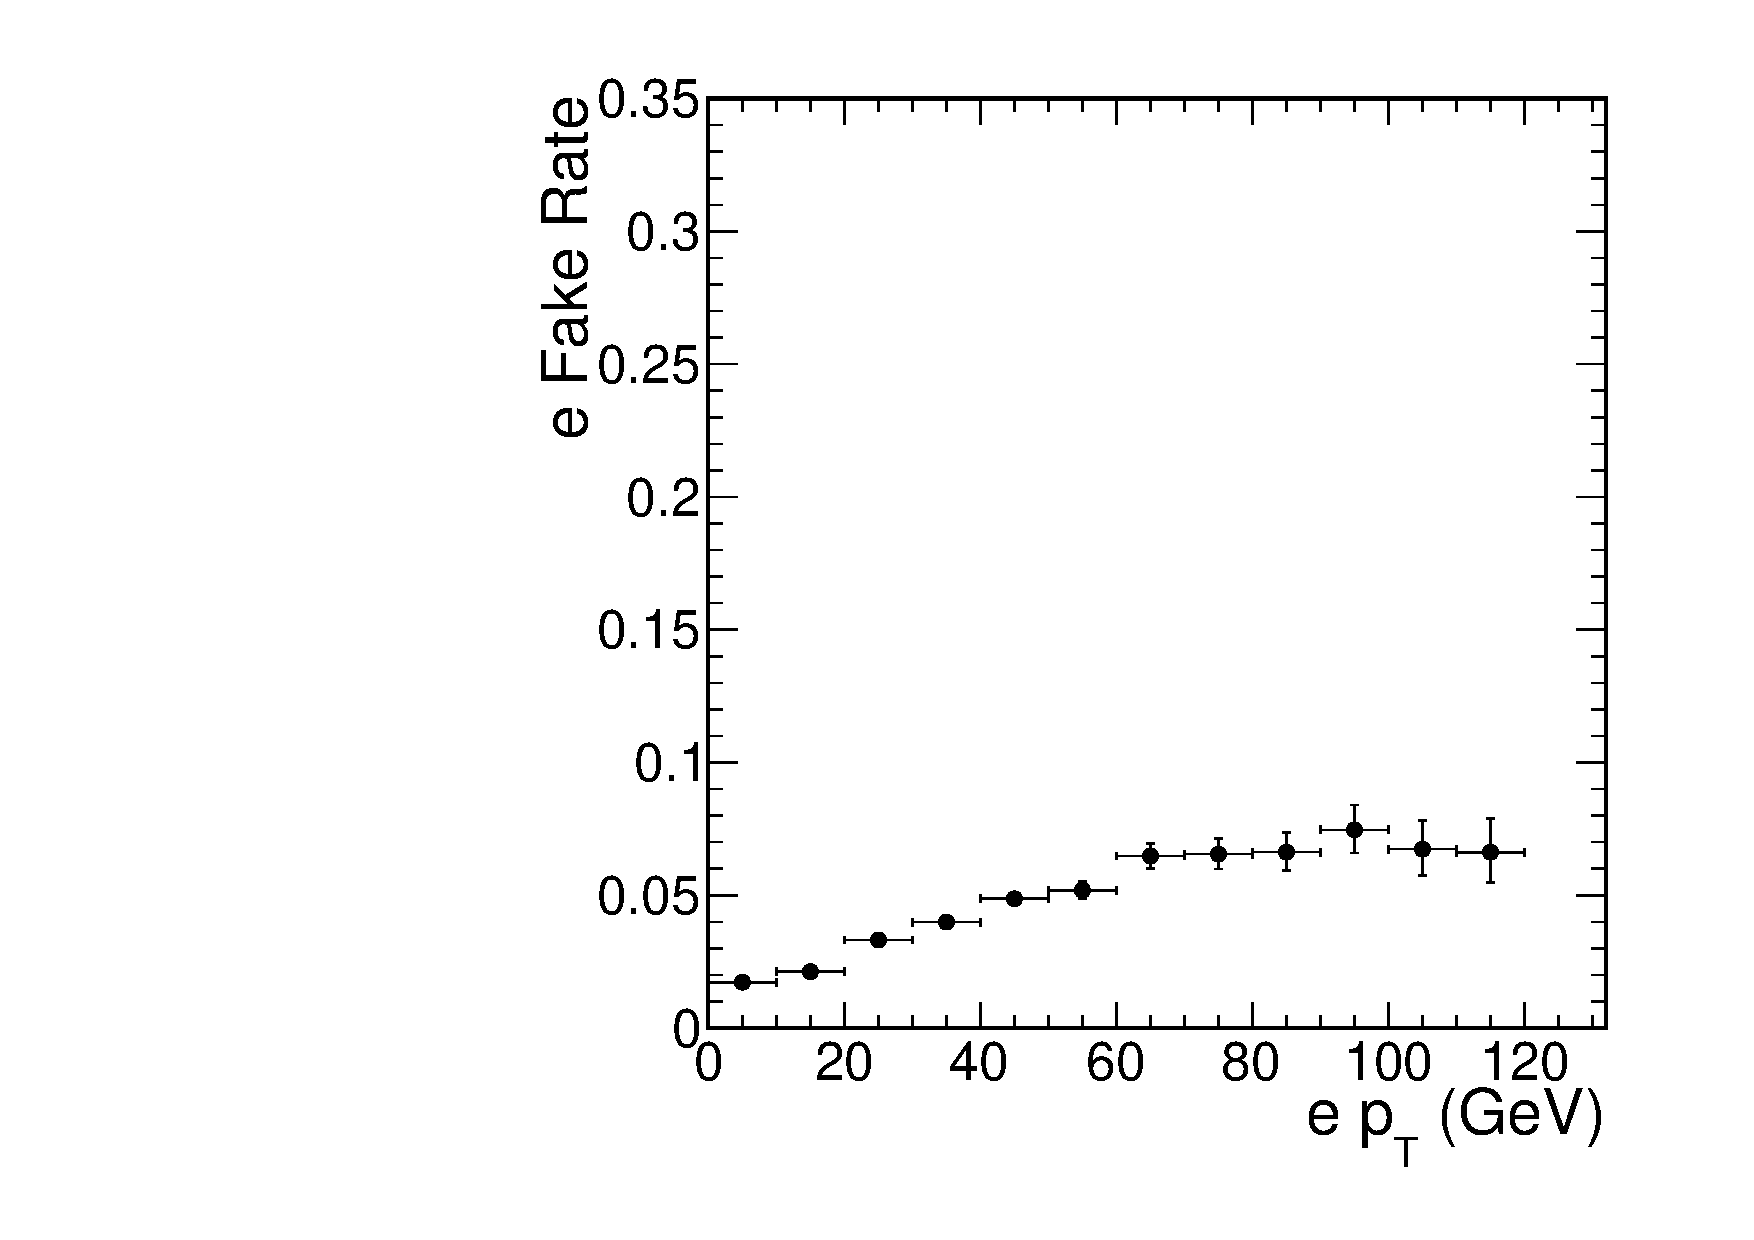
\includegraphics[width=0.45\textwidth]{ele_FR}
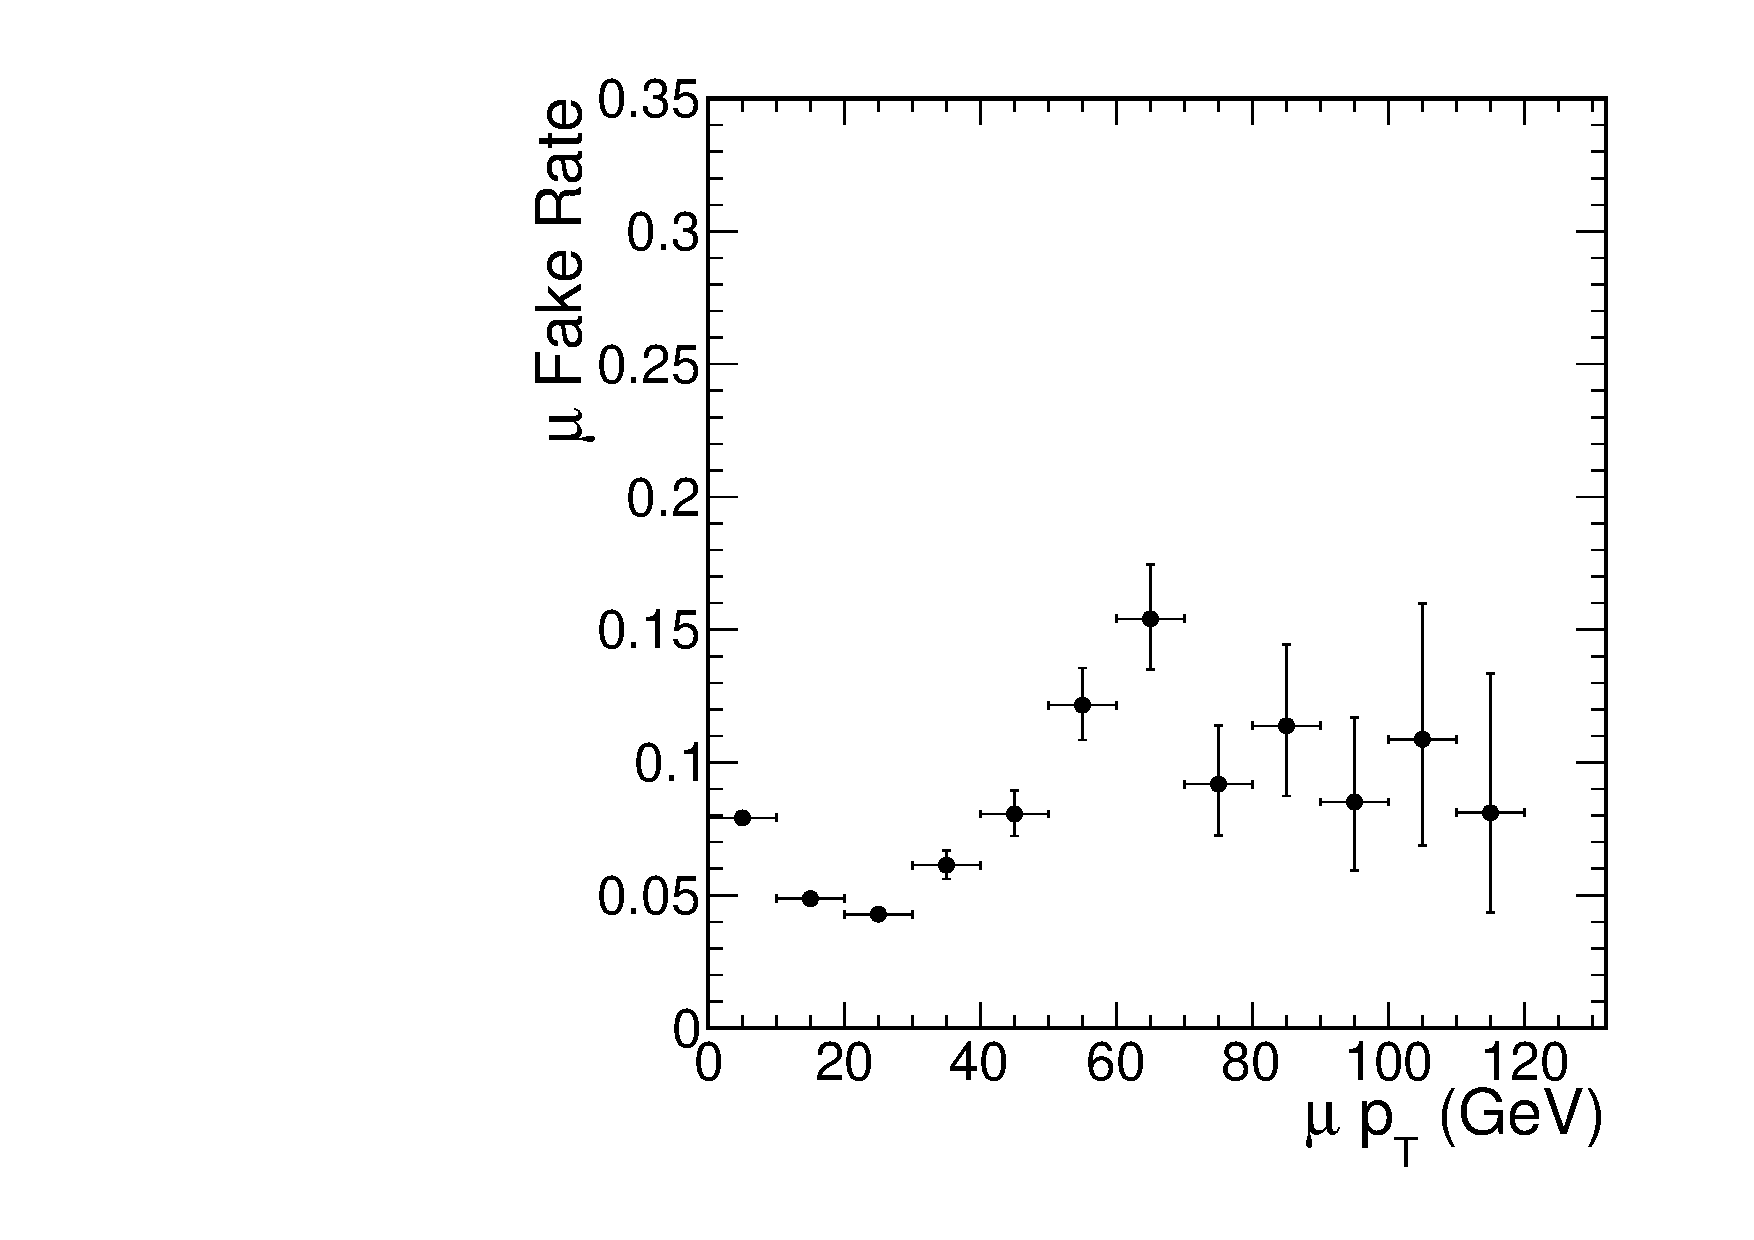
\includegraphics[width=0.45\textwidth]{mu_FR}
\caption[Leptonic fake rates used for the background estimation.]{The leptonic
fake rates, as a function of $p_{T}$ for the electrons (left) and muons (right).}
\label{fig:fakerates}
\end{figure}

In order to estimate the total background contributions due to fakes, potential
backgrounds are split into two separate regions. The first region is
composed of events which contain a fully selected Z, one lepton passing full
selection, and one loose lepton which fails the final selection criteria
(\emph{Z+1P1F}).  These regions are dominated by \Z boson production in
association with two jets, where one of the jets `fakes' a prompt lepton. In
addition, there is a small contribution of W/Z+1 jet production in this region
(though the smaller cross section restricts its impact). The second region is
composed of events with a fully reconstructed \Z boson plus two additional loose
leptons, both of which fail the final selection criteria (\emph{Z+2F}). This region is
composed almost entirely of \Z boson production. There is a negligible contamination
of ZZ in each of these regions. The population for these regions for each of the
final states (plus the combination) is shown in figures~\ref{fig:AAregions}
and~\ref{fig:AIregions}. The statistics in the simulated Drell-Yan sample has
limited statistics when an on-shell Z is required (as seen in
figures~\ref{fig:AAregions_highmass} and~\ref{fig:AIregions_highmass}). However,
the overall successful modelling of these control regions with the looser mass
requirements (Figures~\ref{fig:AAregions} and \ref{fig:AIregions}) gives confidence
in the method, as the expected physics processes are the same regardless of the
mass requirement.

\begin{figure}[h]
\centering
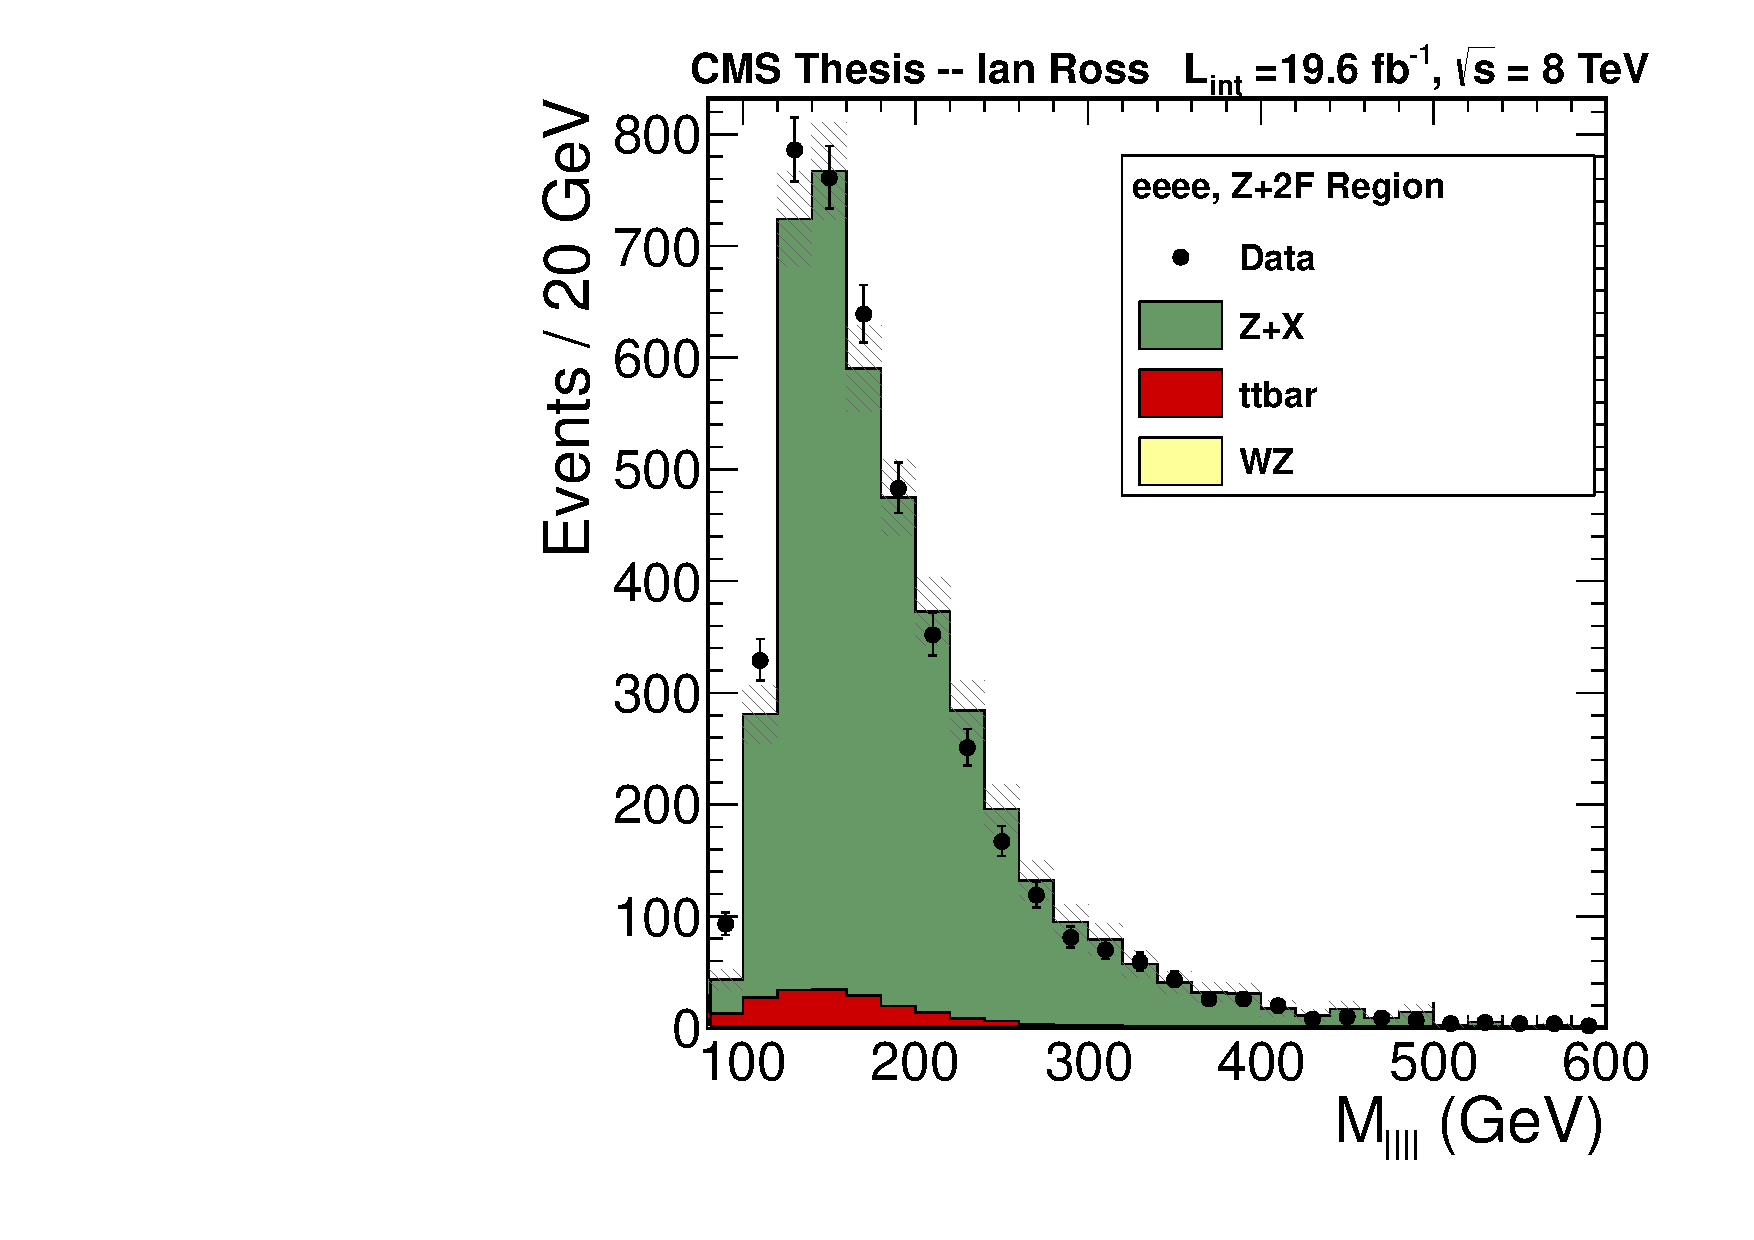
\includegraphics[width=0.45\textwidth]{eeee_AA}
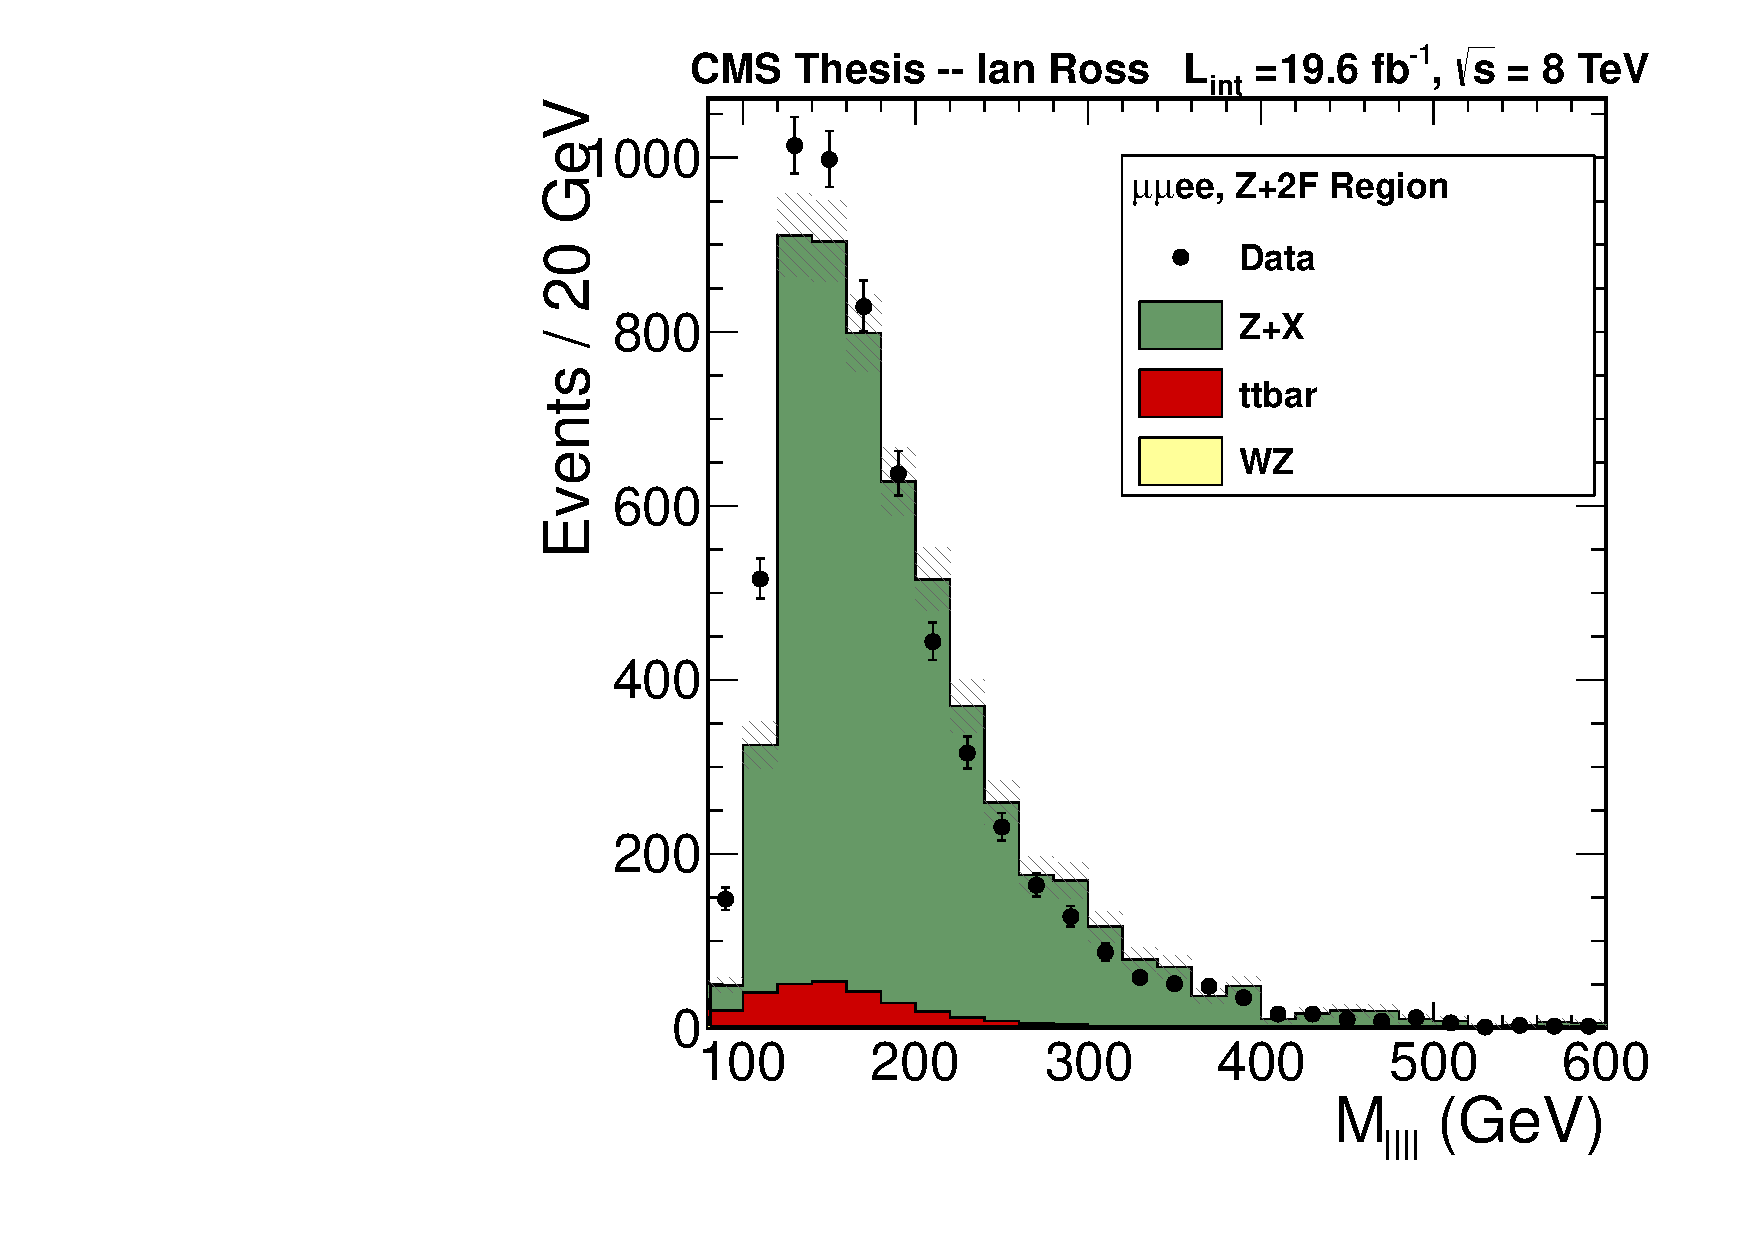
\includegraphics[width=0.45\textwidth]{mmee_AA}\\
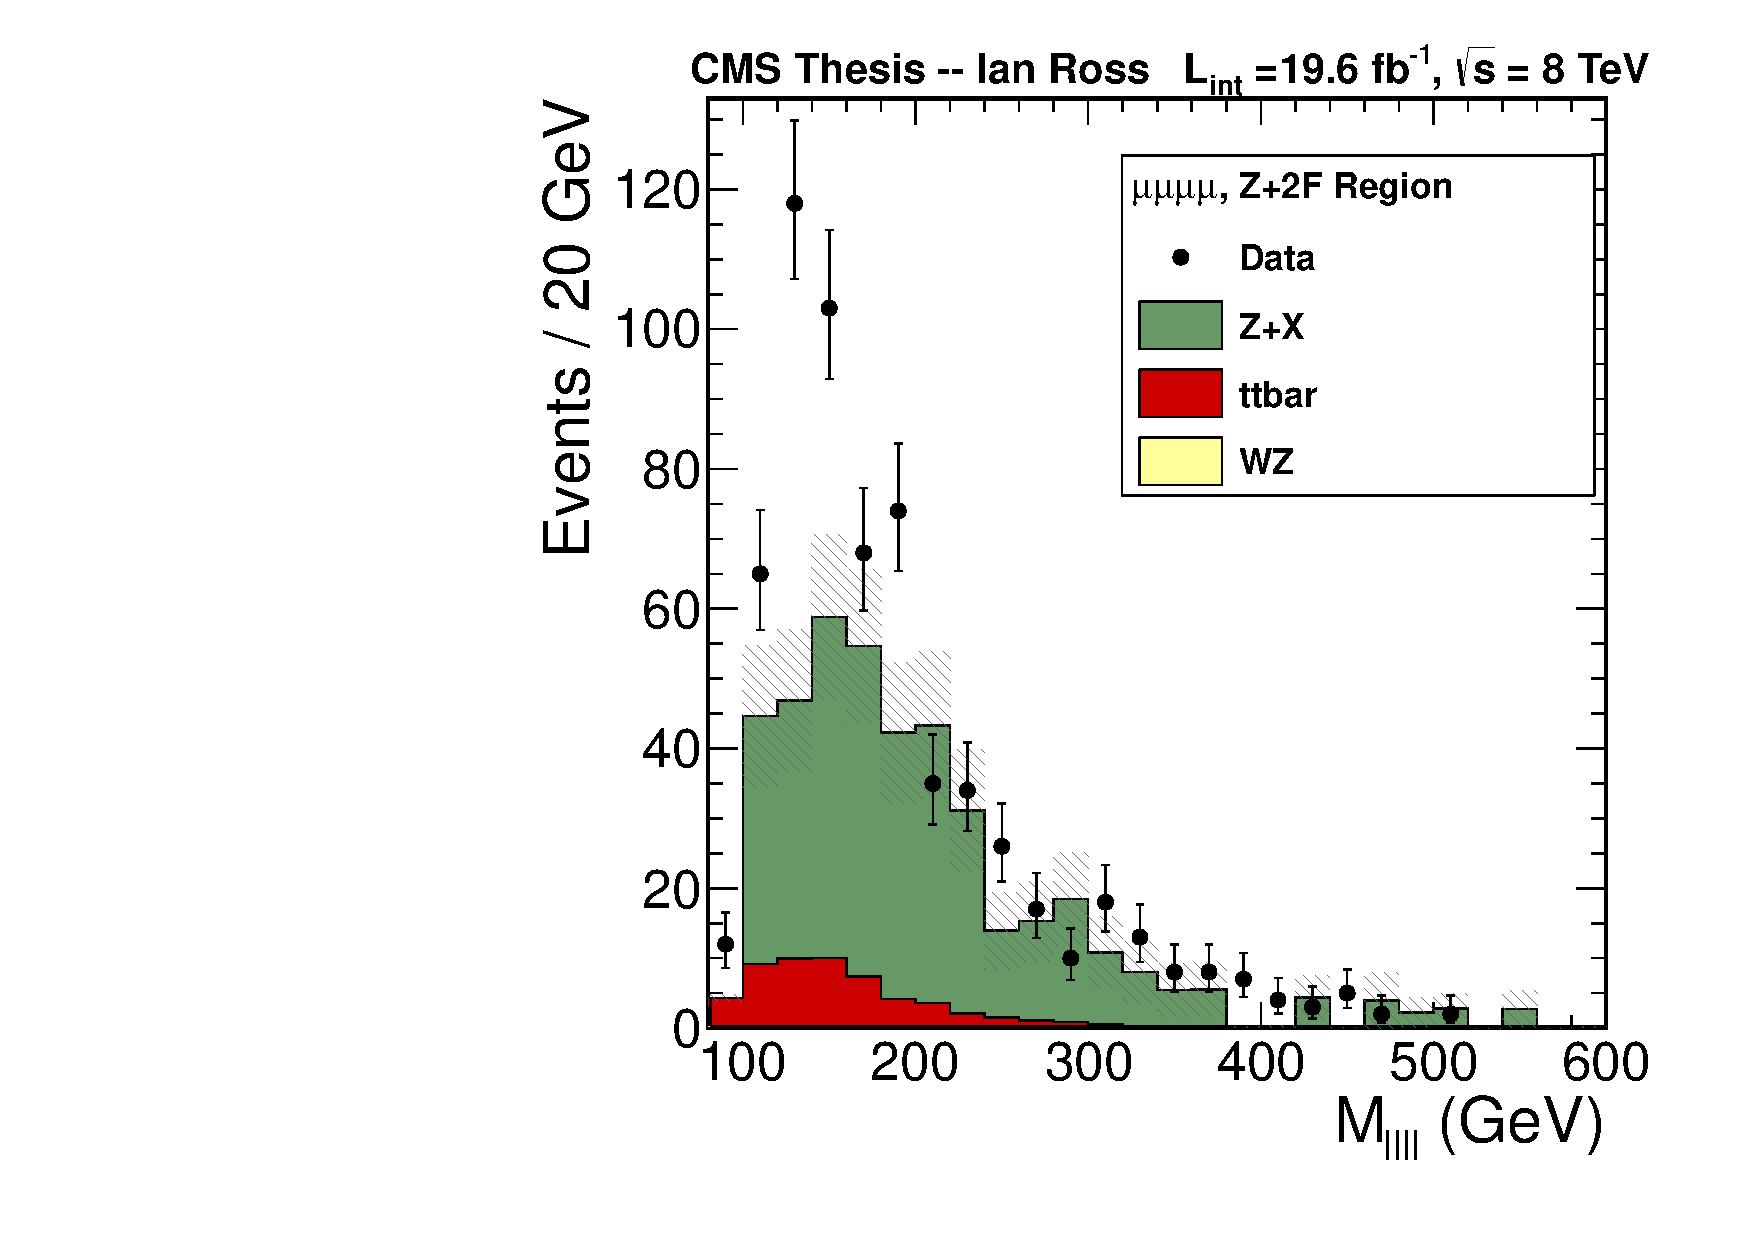
\includegraphics[width=0.45\textwidth]{mmmm_AA}
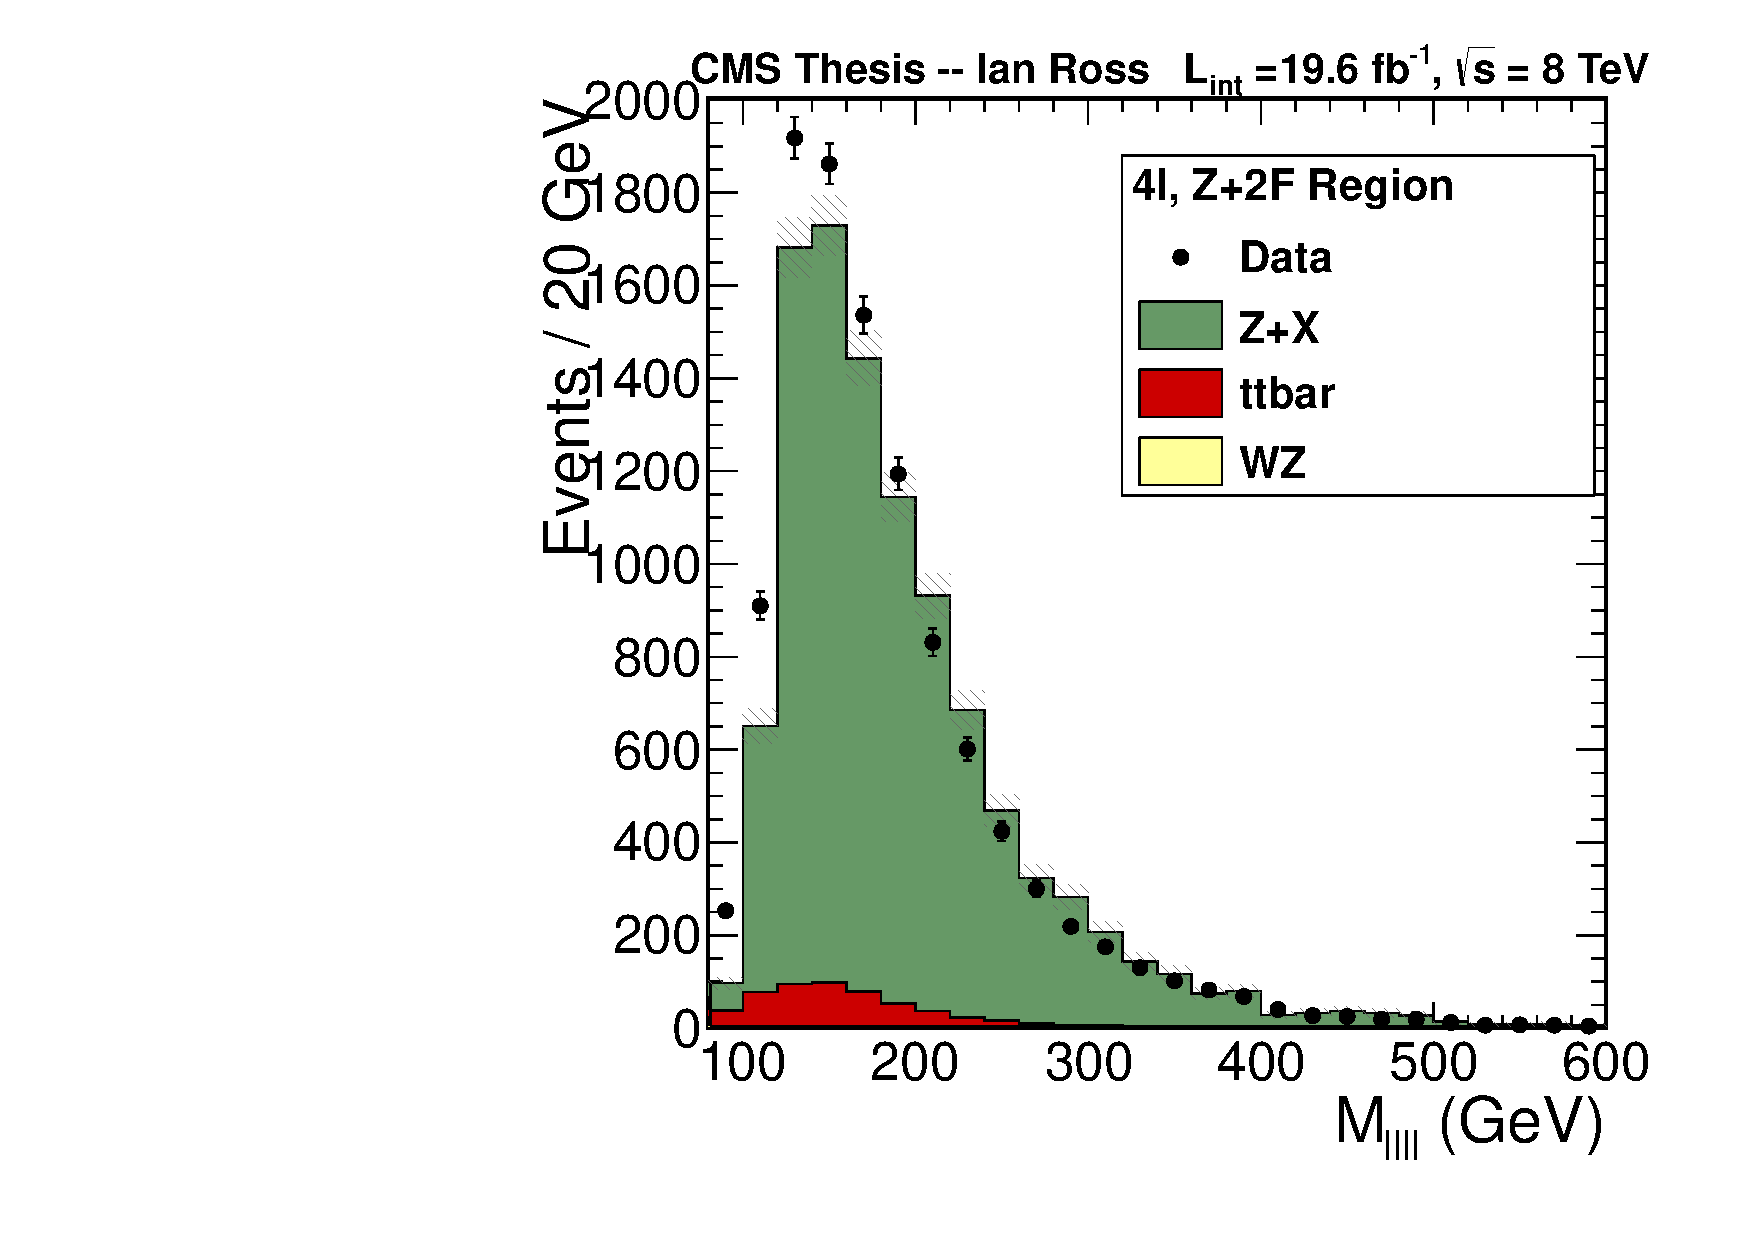
\includegraphics[width=0.45\textwidth]{4l_AA}\\
\caption[Background estimation region consisting of a \Z plus two failed
leptons.]{Background estimation region consisting of a \Z plus two failed
leptons. Counter clockwise from top right is the eeee, $\mu\mu ee$,
$\mu\mu\mu\mu$, and summed final states.}
\label{fig:AAregions}
\end{figure}

\begin{figure}[h]
\centering
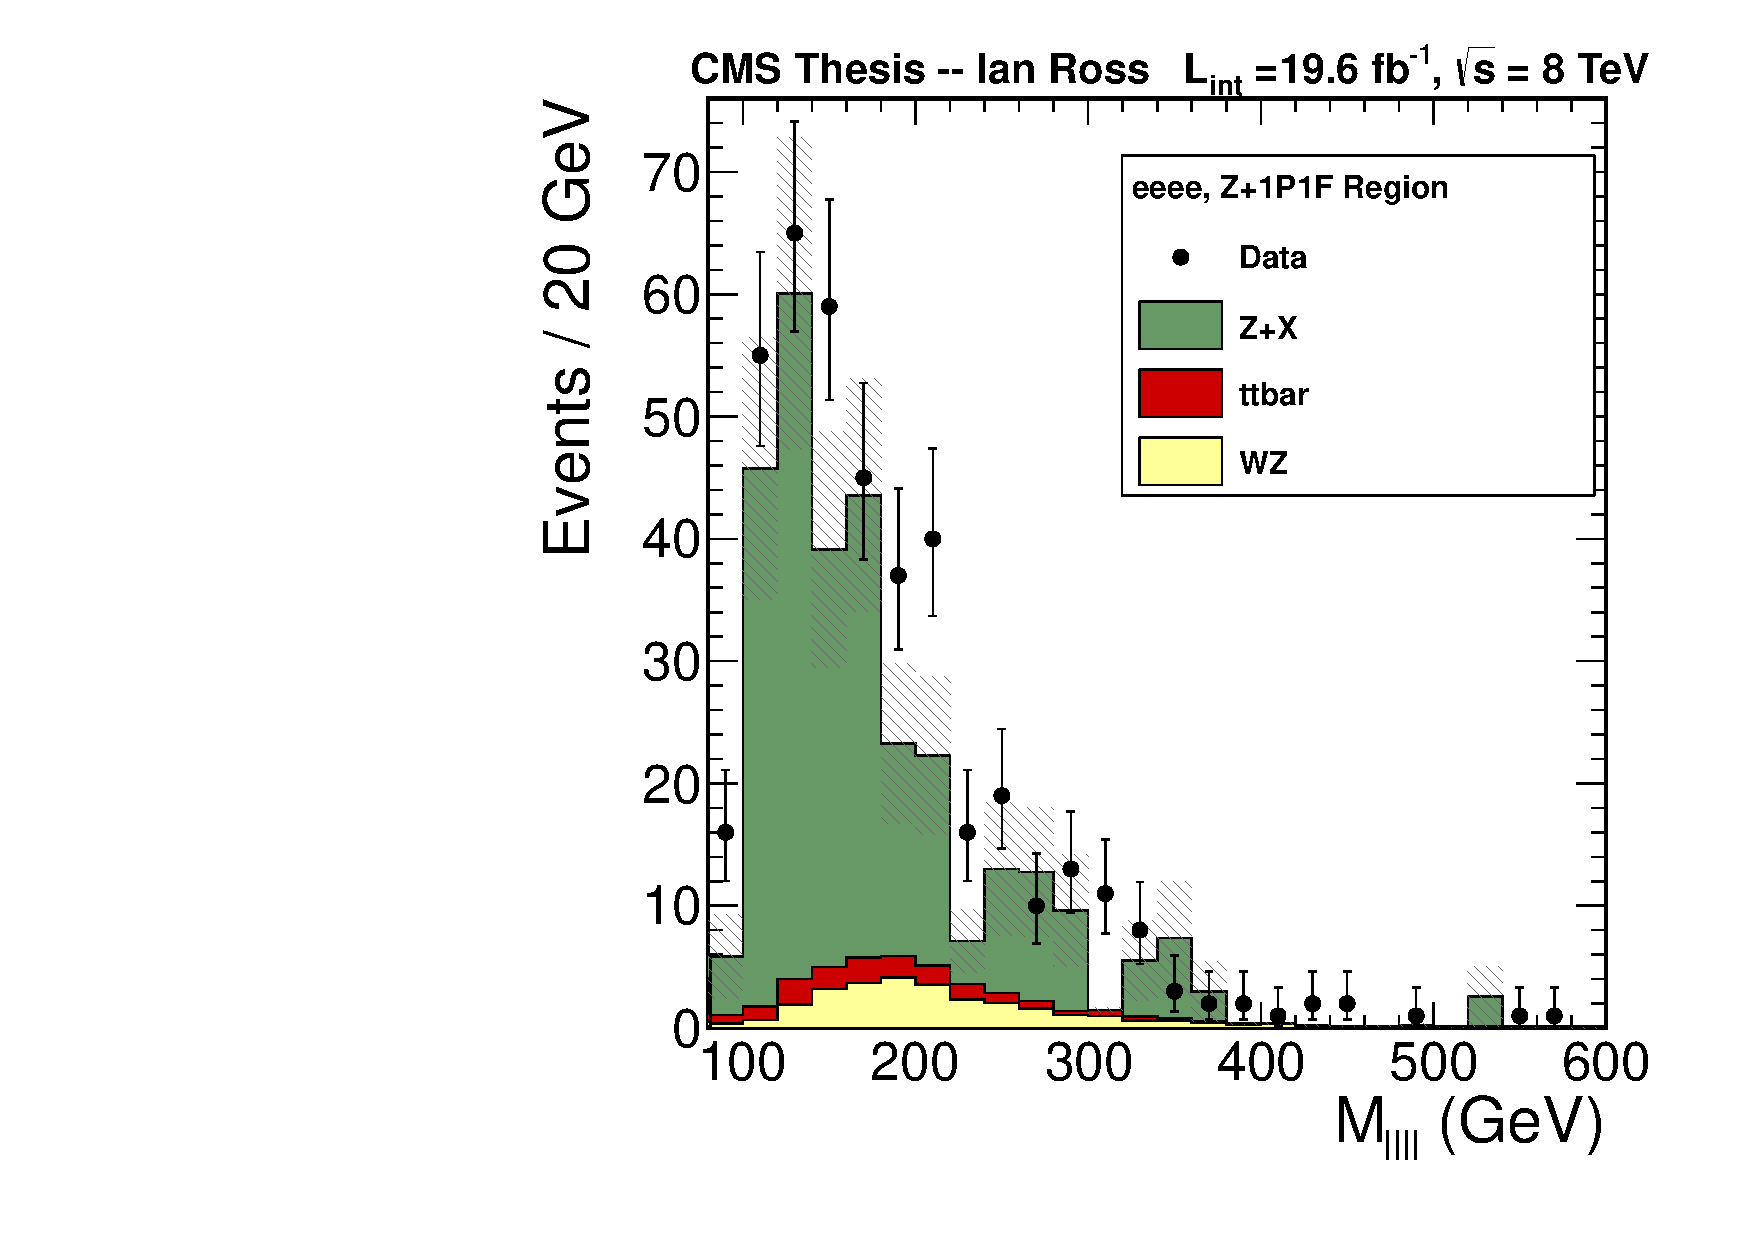
\includegraphics[width=0.45\textwidth]{eeee_IA}
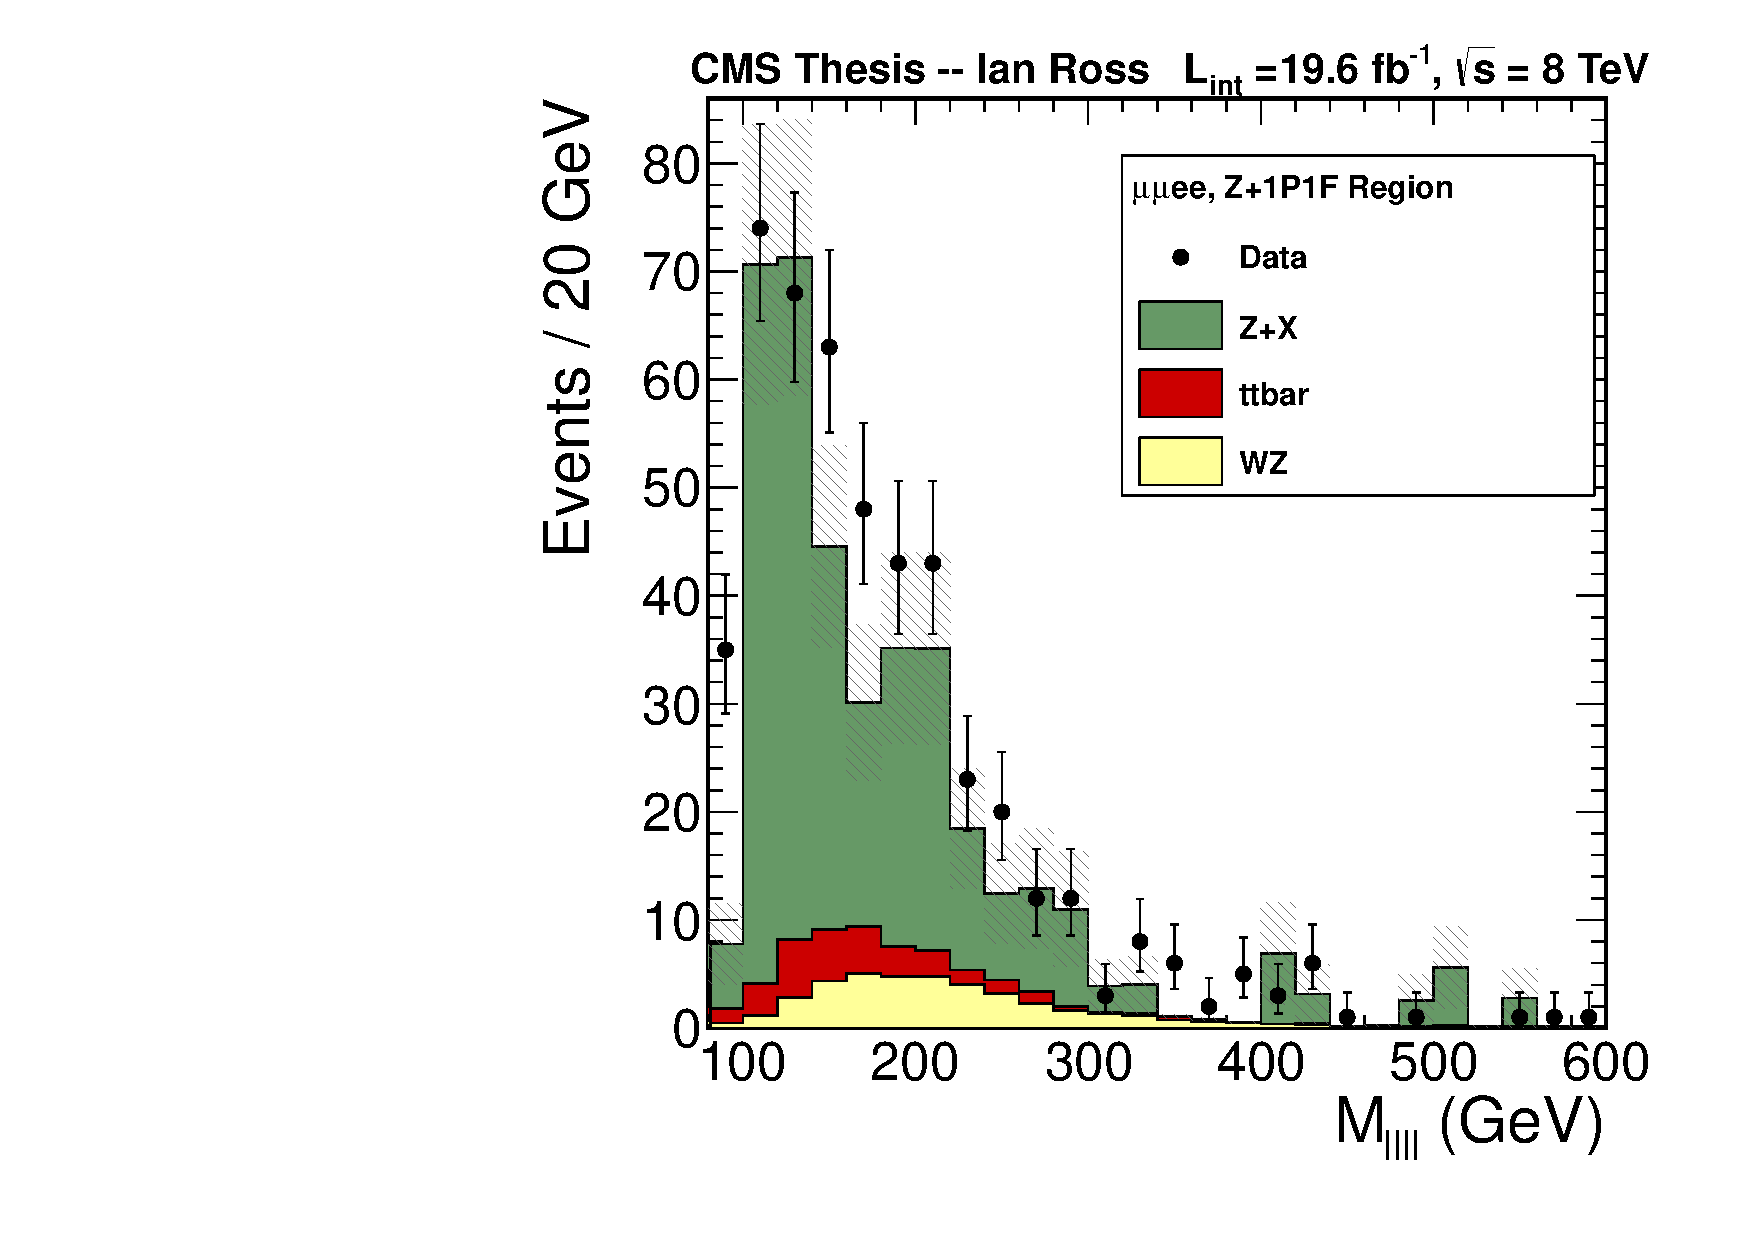
\includegraphics[width=0.45\textwidth]{mmee_IA}\\
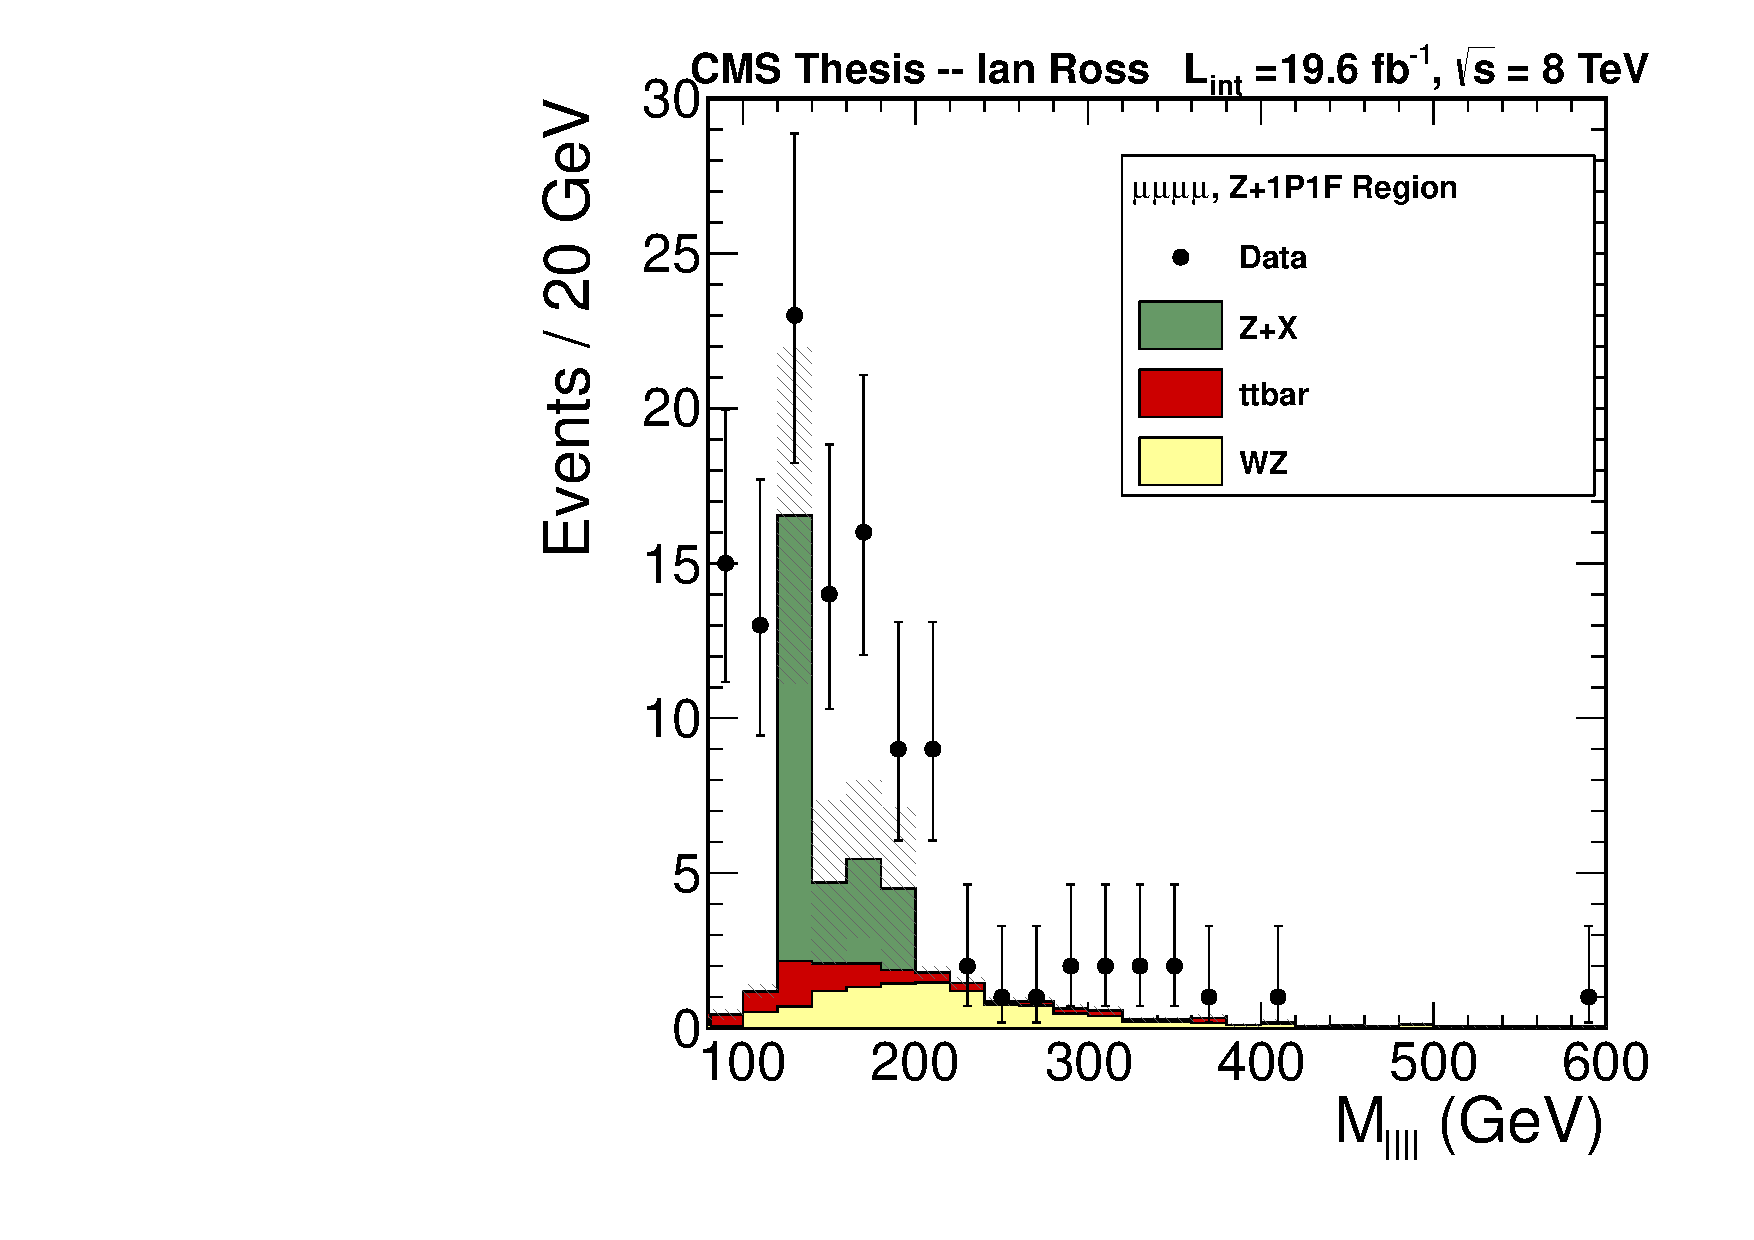
\includegraphics[width=0.45\textwidth]{mmmm_IA}
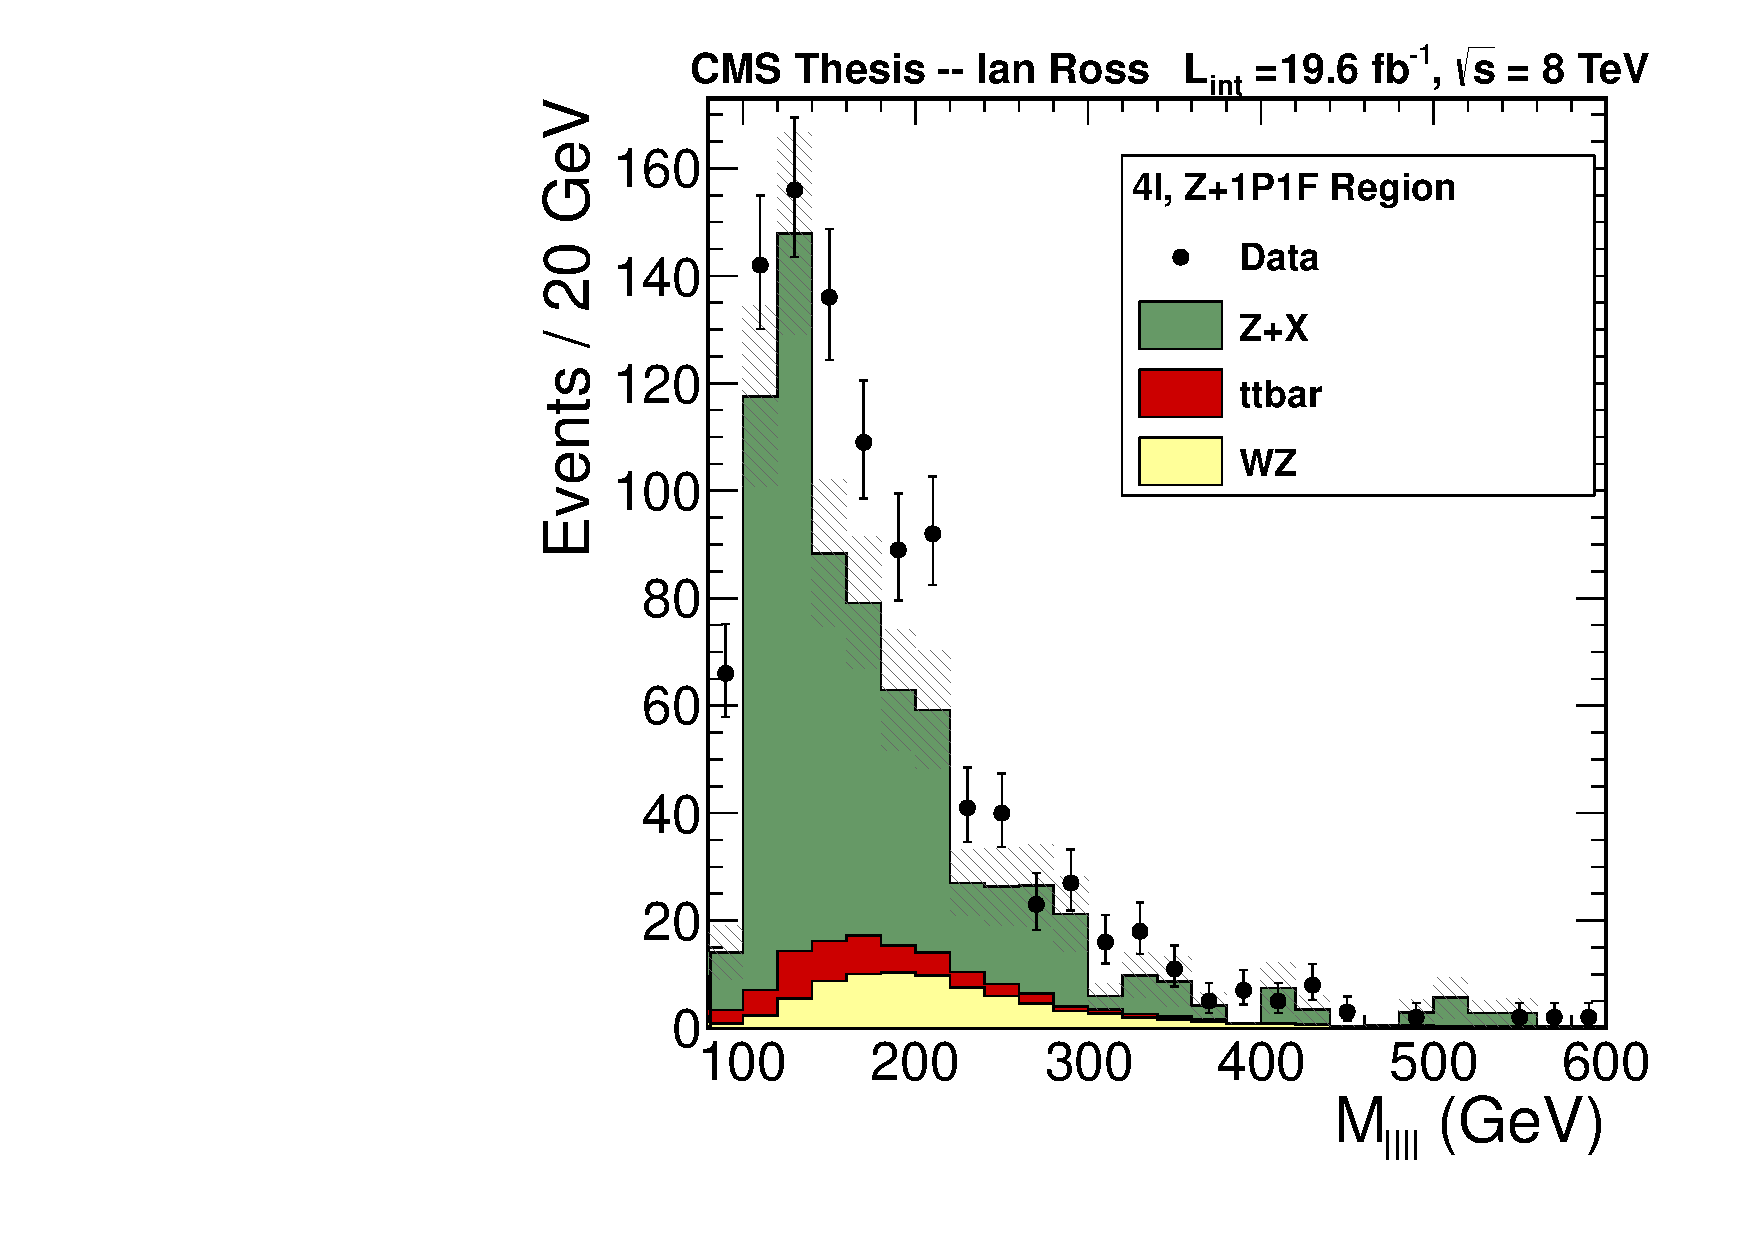
\includegraphics[width=0.45\textwidth]{4l_IA}\\
\caption[Background estimation region consisting of a \Z plus one passed and one failed
leptons.]{Background estimation region consisting of a \Z plus one passed and
    one failed leptons. Counter clockwise from top right is the eeee, $\mu\mu
    ee$, $\mu\mu\mu\mu$, and summed final states.}
\label{fig:AIregions}
\end{figure}

\begin{figure}[h]
\centering
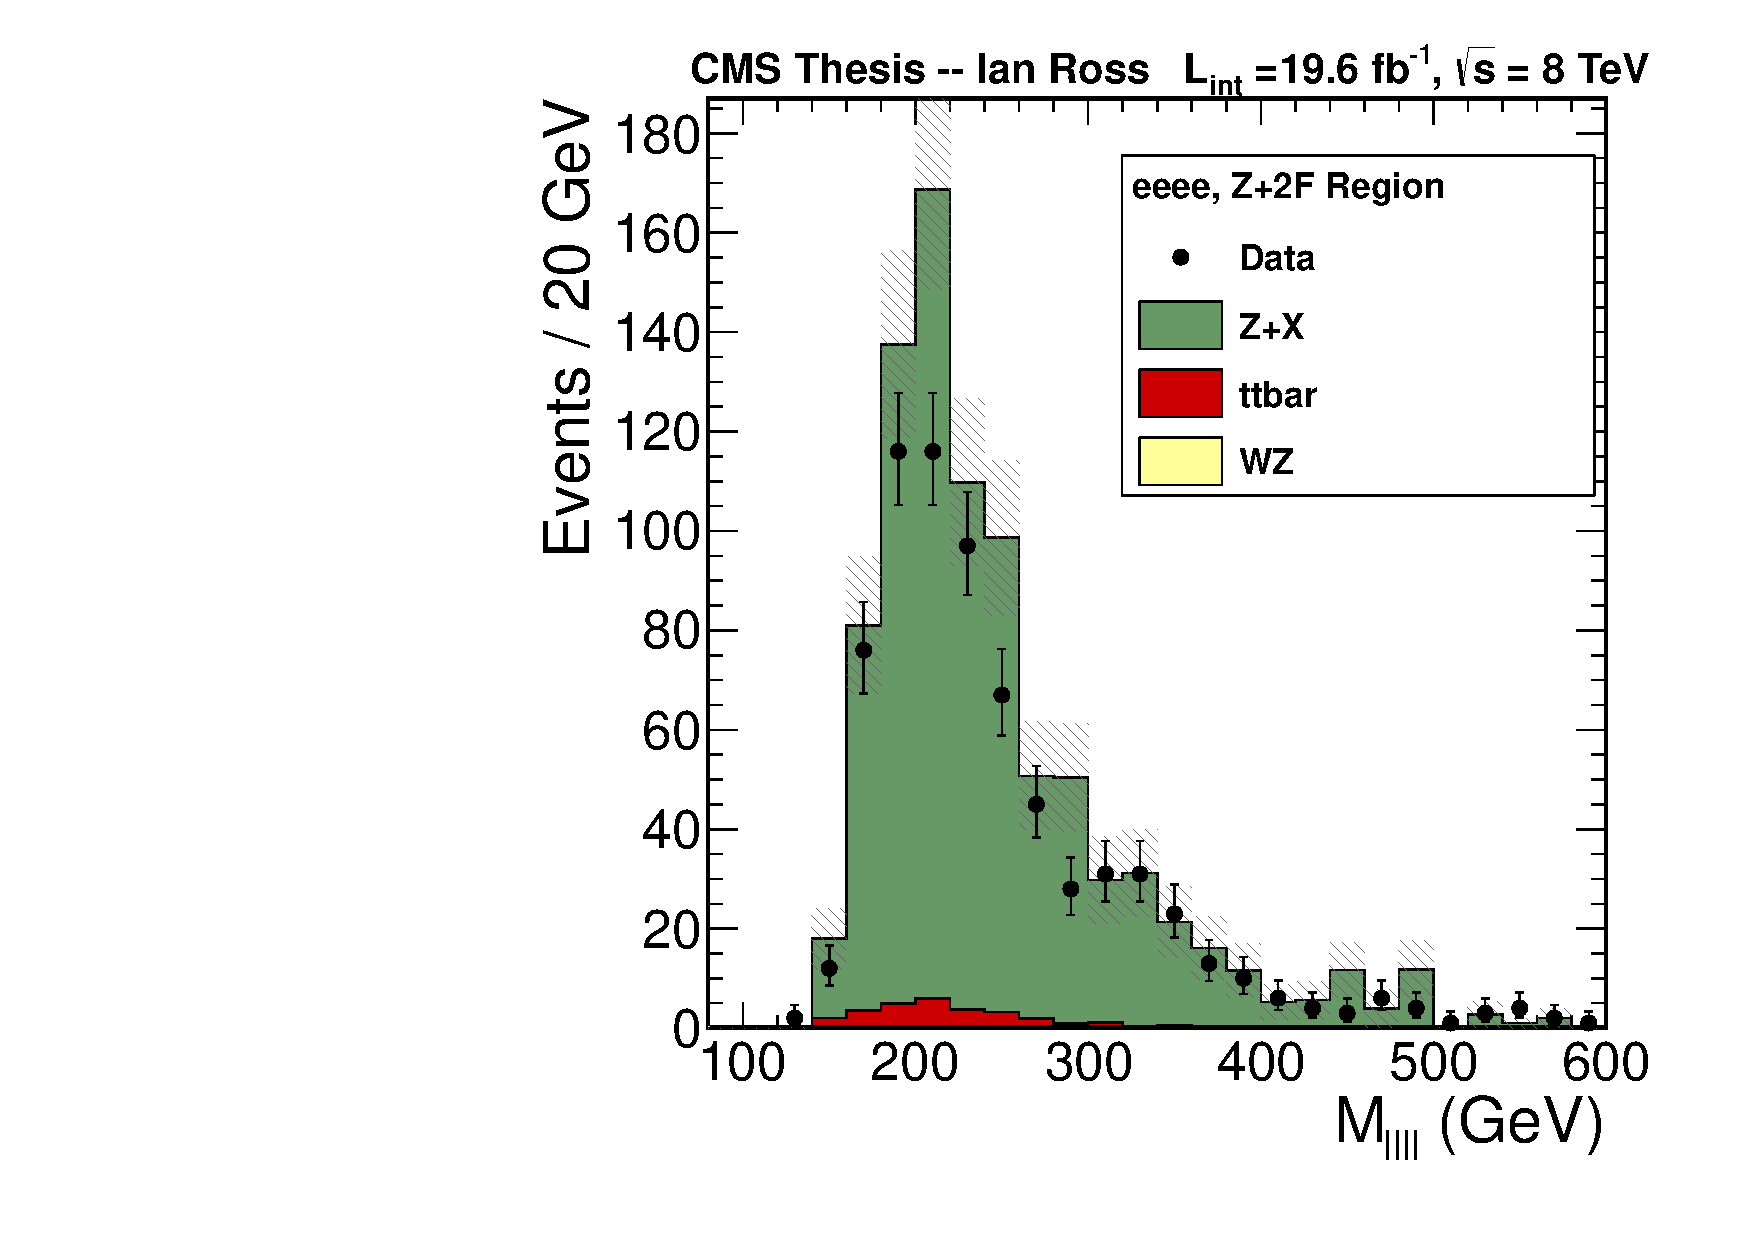
\includegraphics[width=0.45\textwidth]{eeee_AA_highmass}
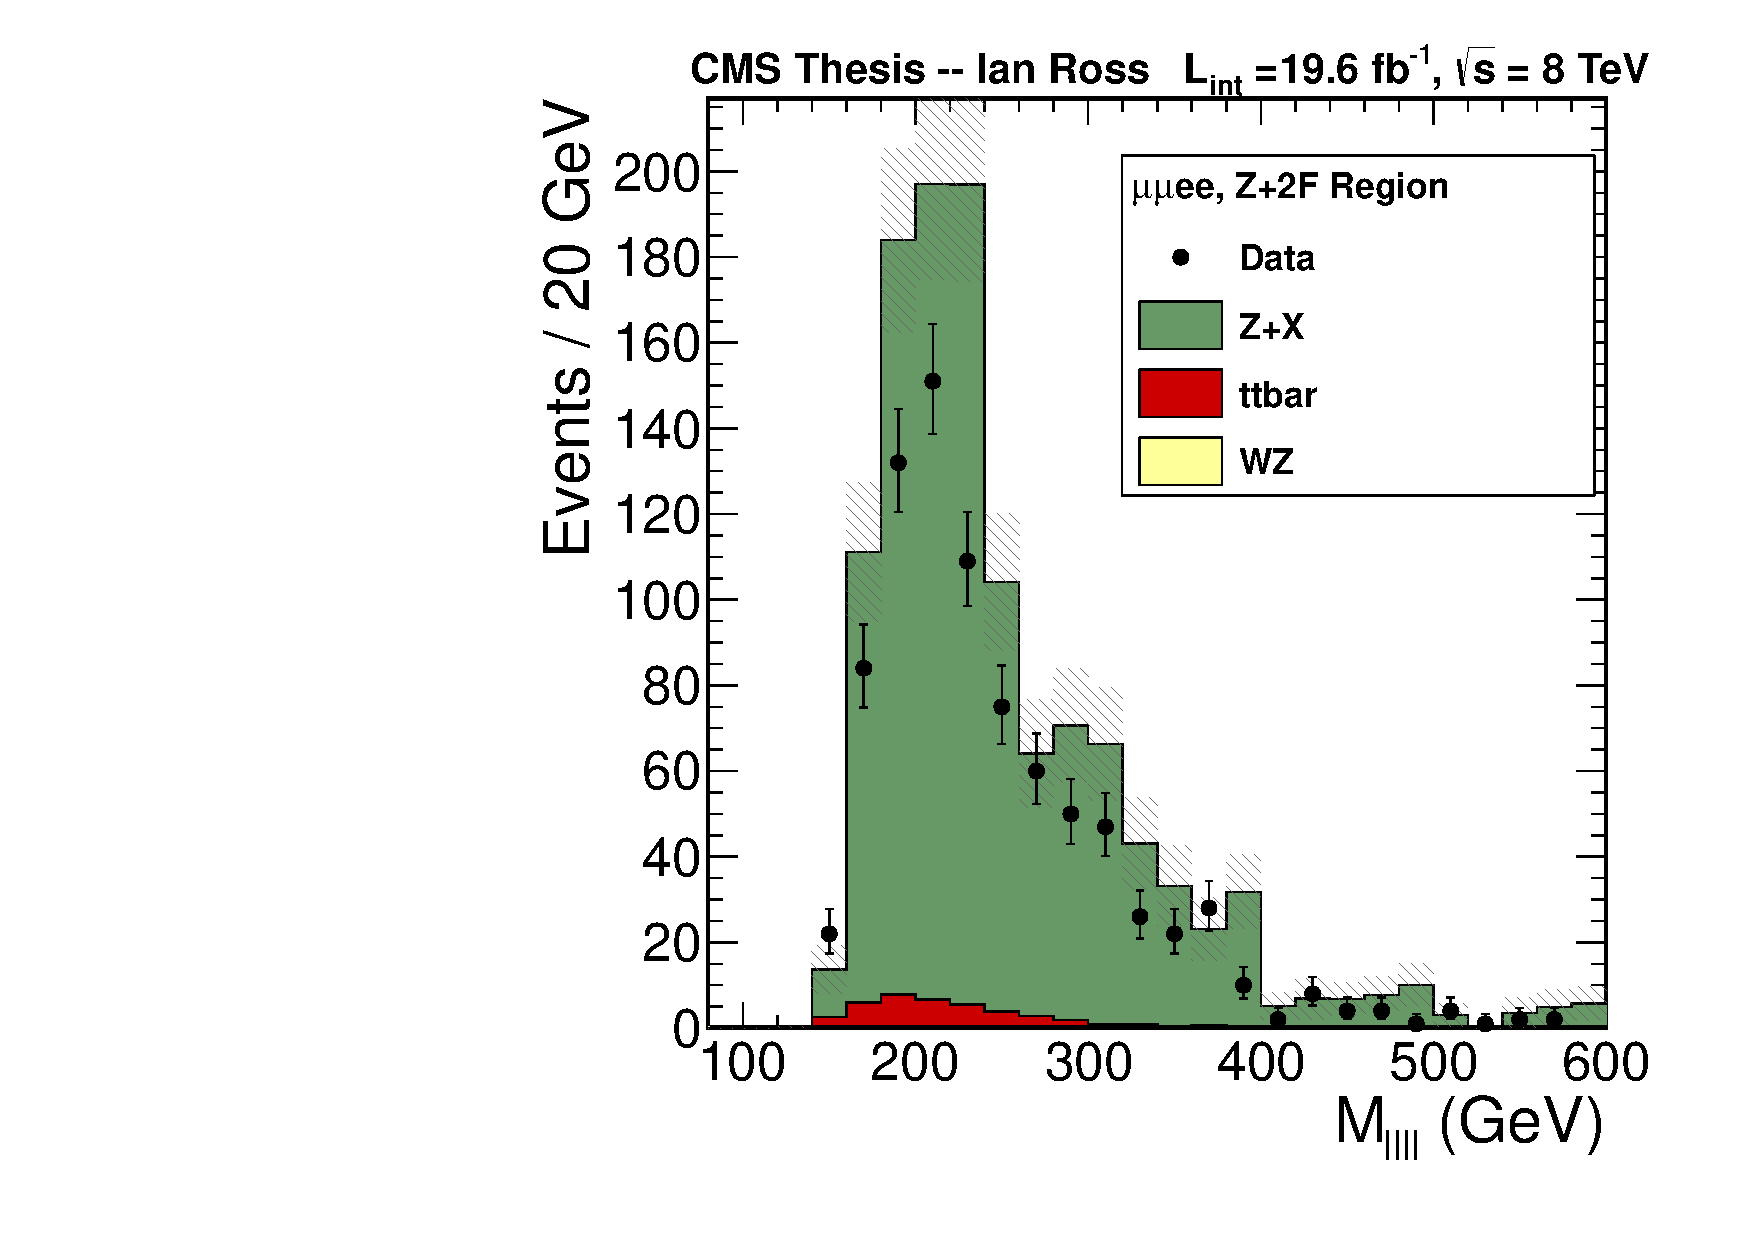
\includegraphics[width=0.45\textwidth]{mmee_AA_highmass}\\
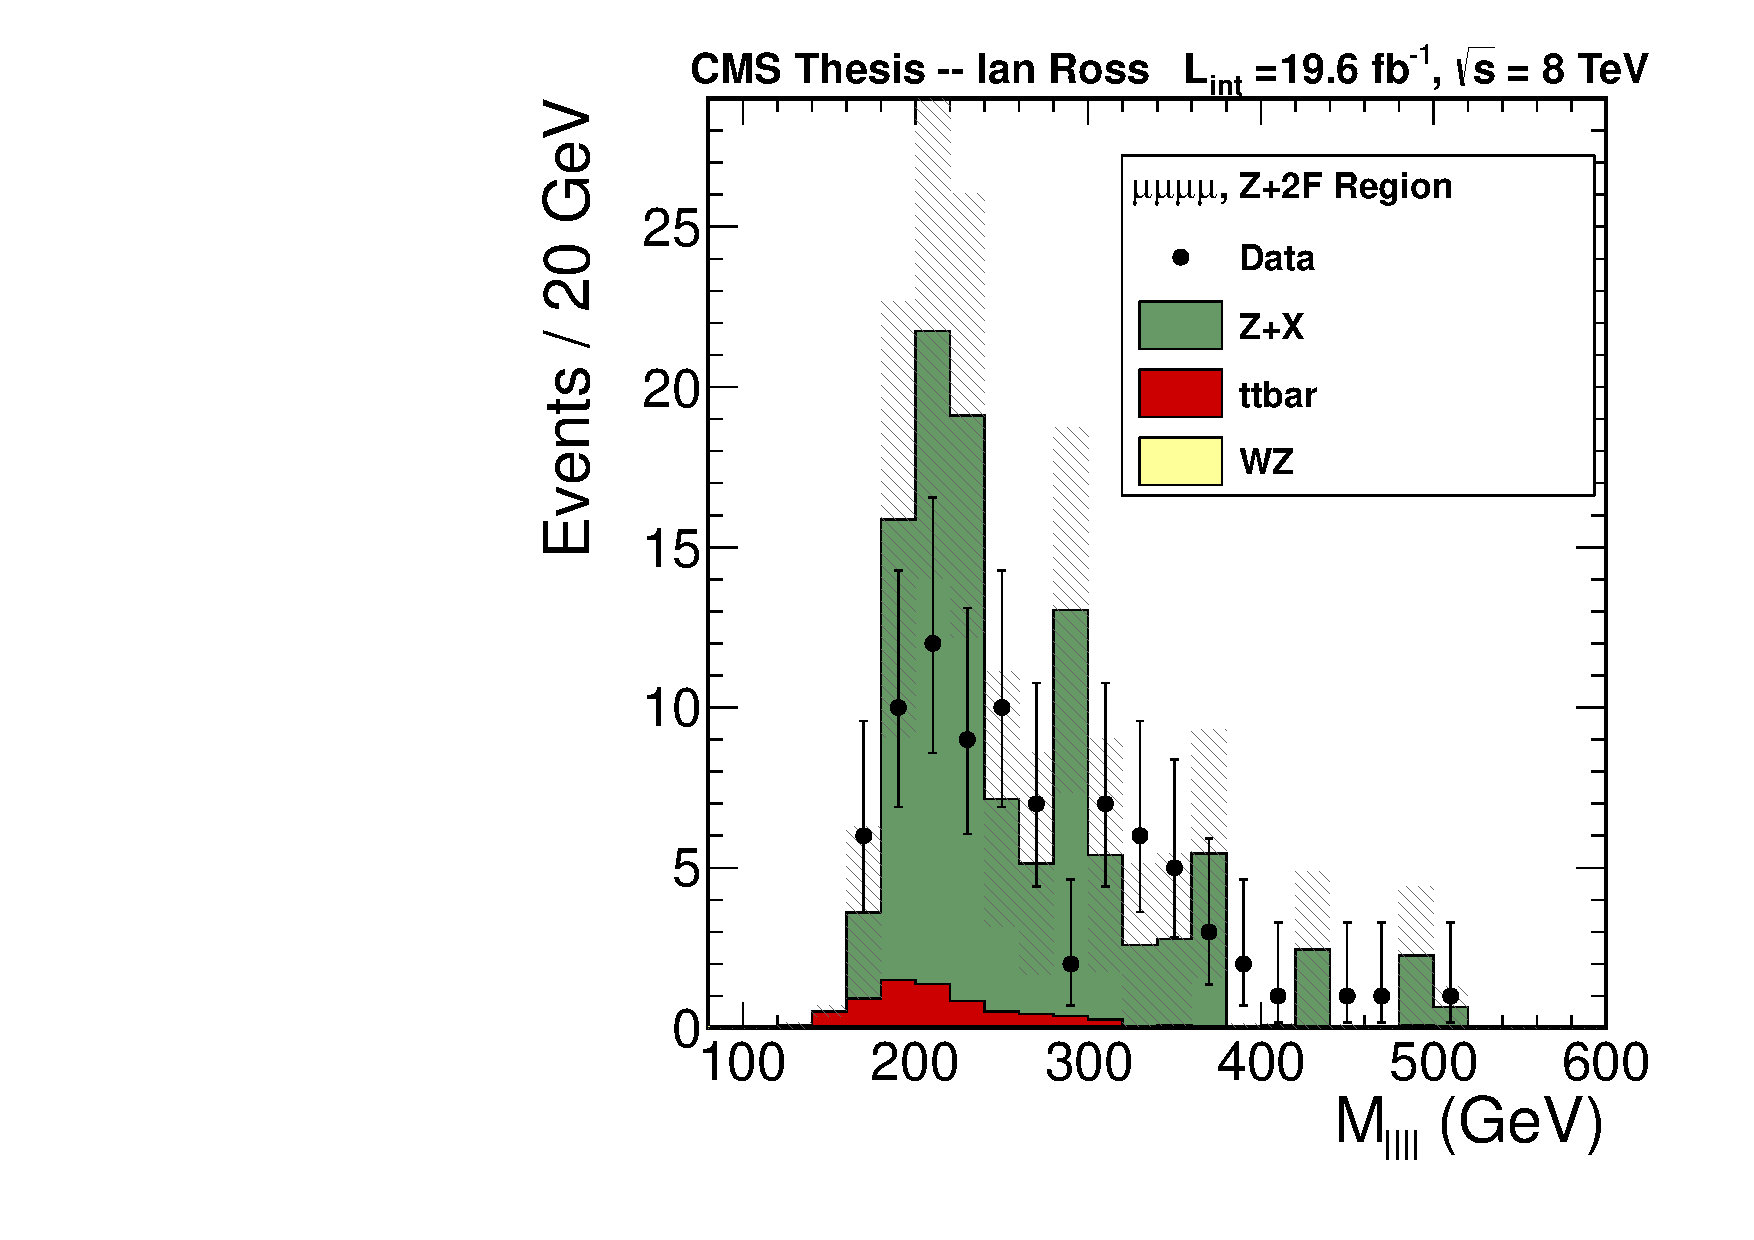
\includegraphics[width=0.45\textwidth]{mmmm_AA_highmass}
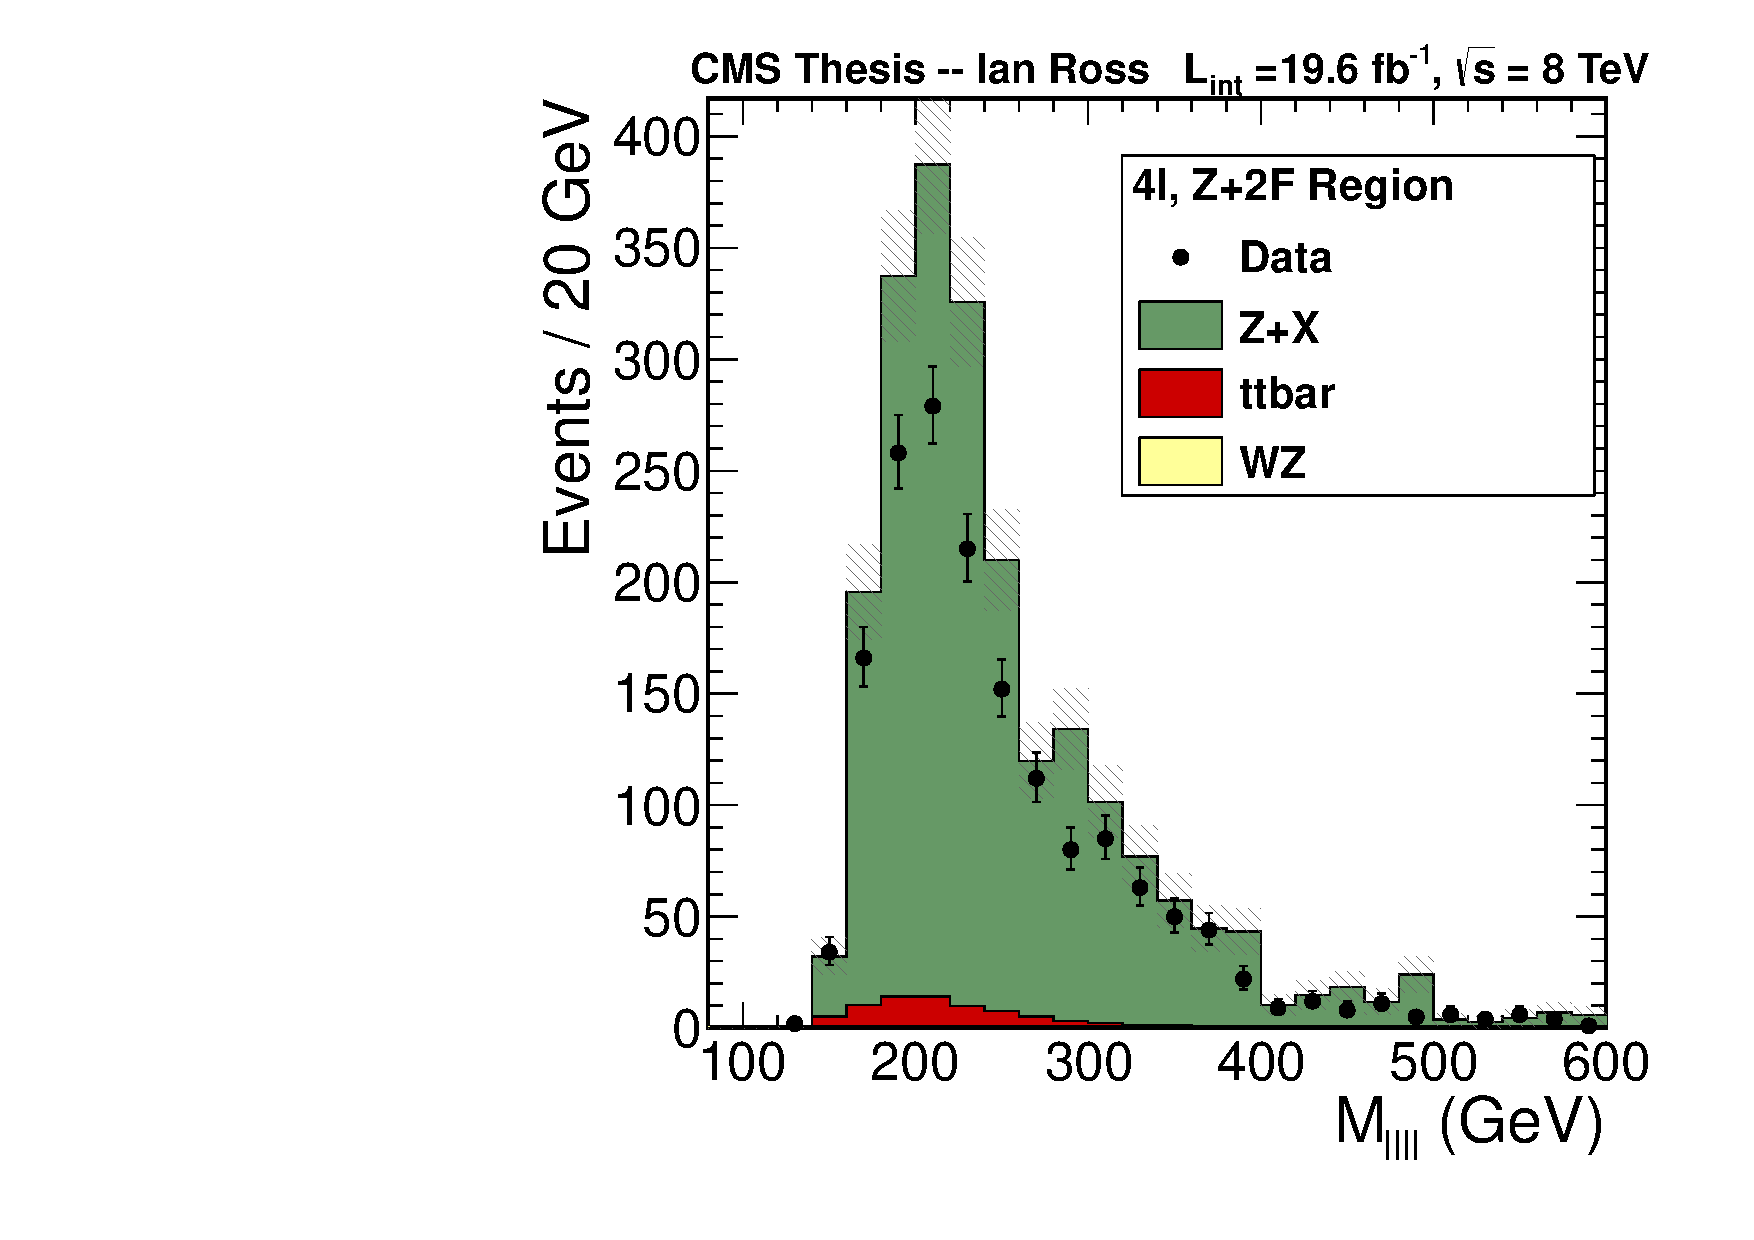
\includegraphics[width=0.45\textwidth]{4l_AA_highmass}\\
\caption[Background estimation region consisting of a \Z plus two failed
leptons, with the high mass requirement.]{Background estimation region consisting of a \Z plus two failed
leptons, with the high mass requirement. Counter clockwise from top right is the eeee, $\mu\mu ee$,
$\mu\mu\mu\mu$, and summed final states.}
\label{fig:AAregions_highmass}
\end{figure}

\begin{figure}[h]
\centering
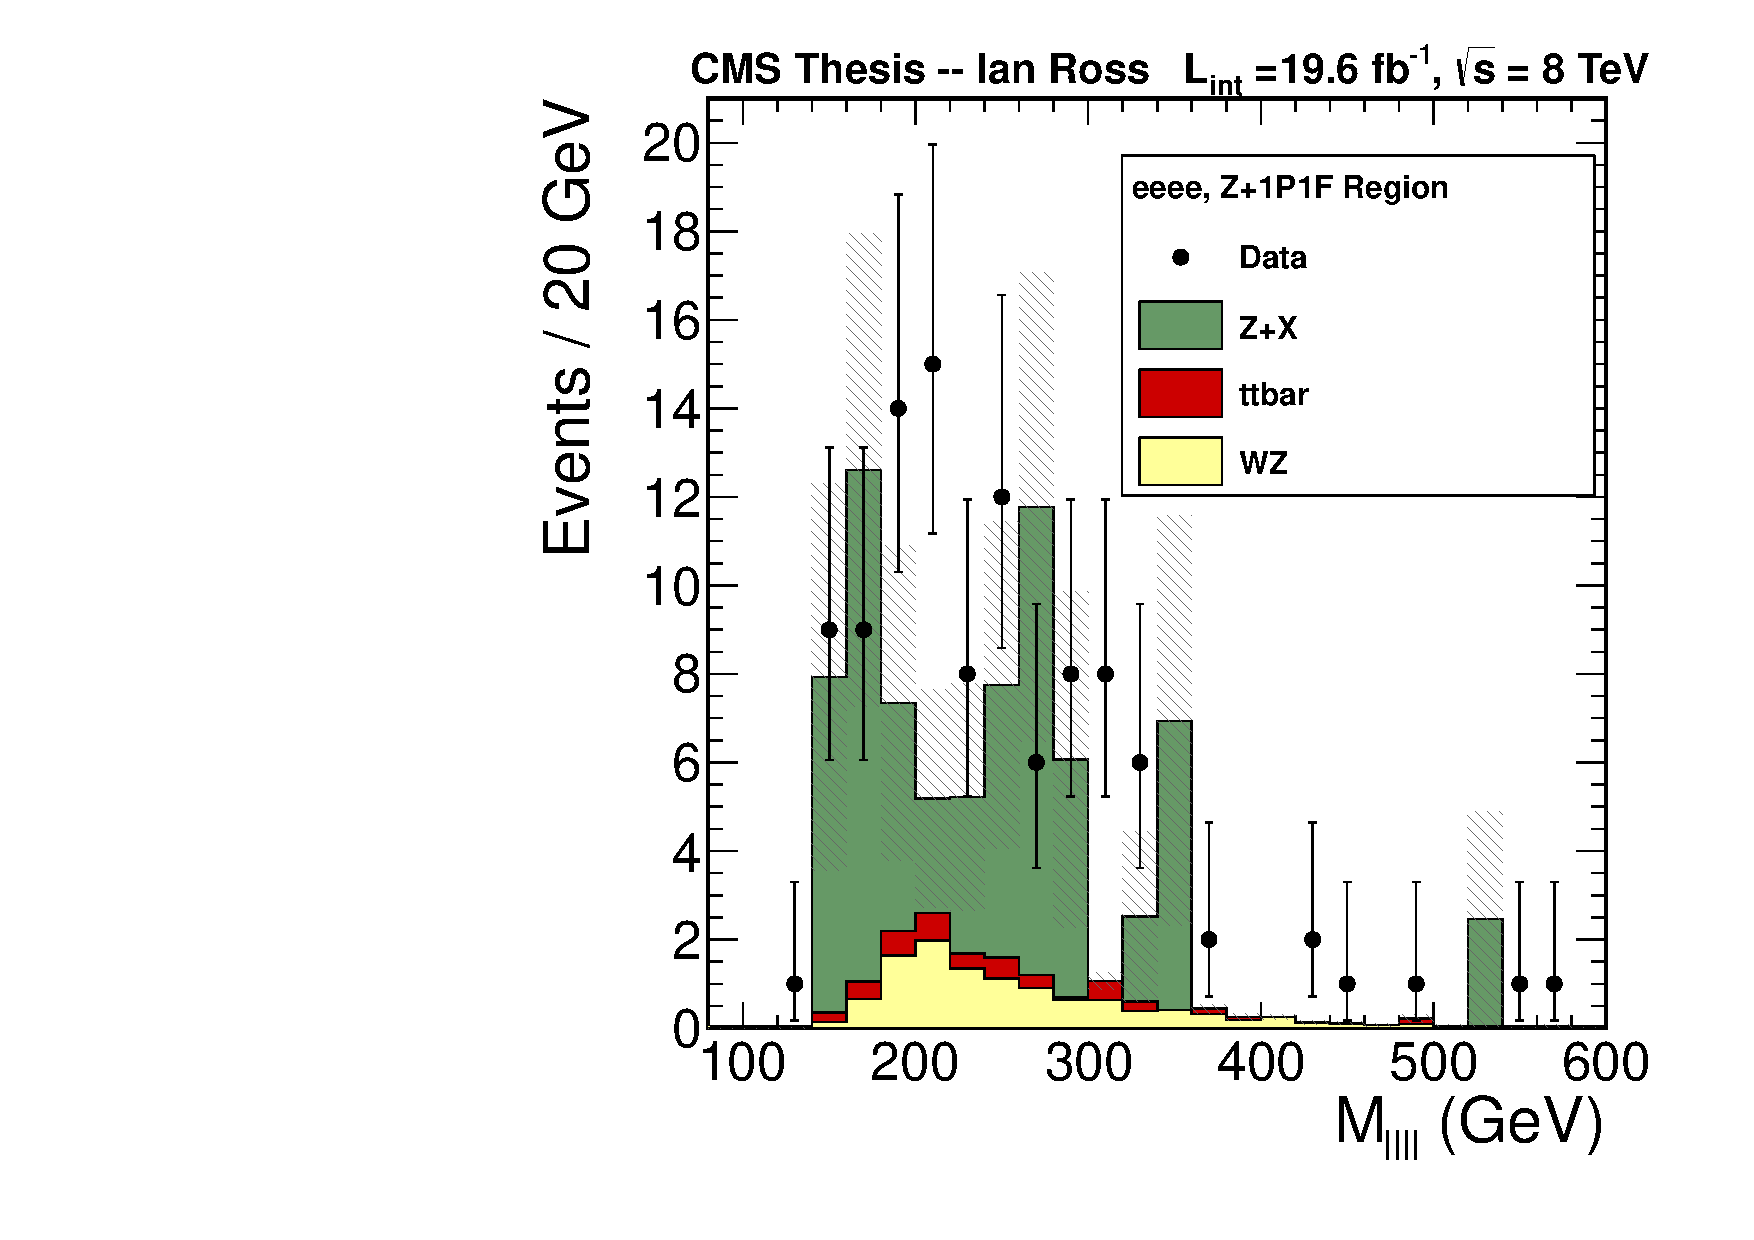
\includegraphics[width=0.45\textwidth]{eeee_IA_highmass}
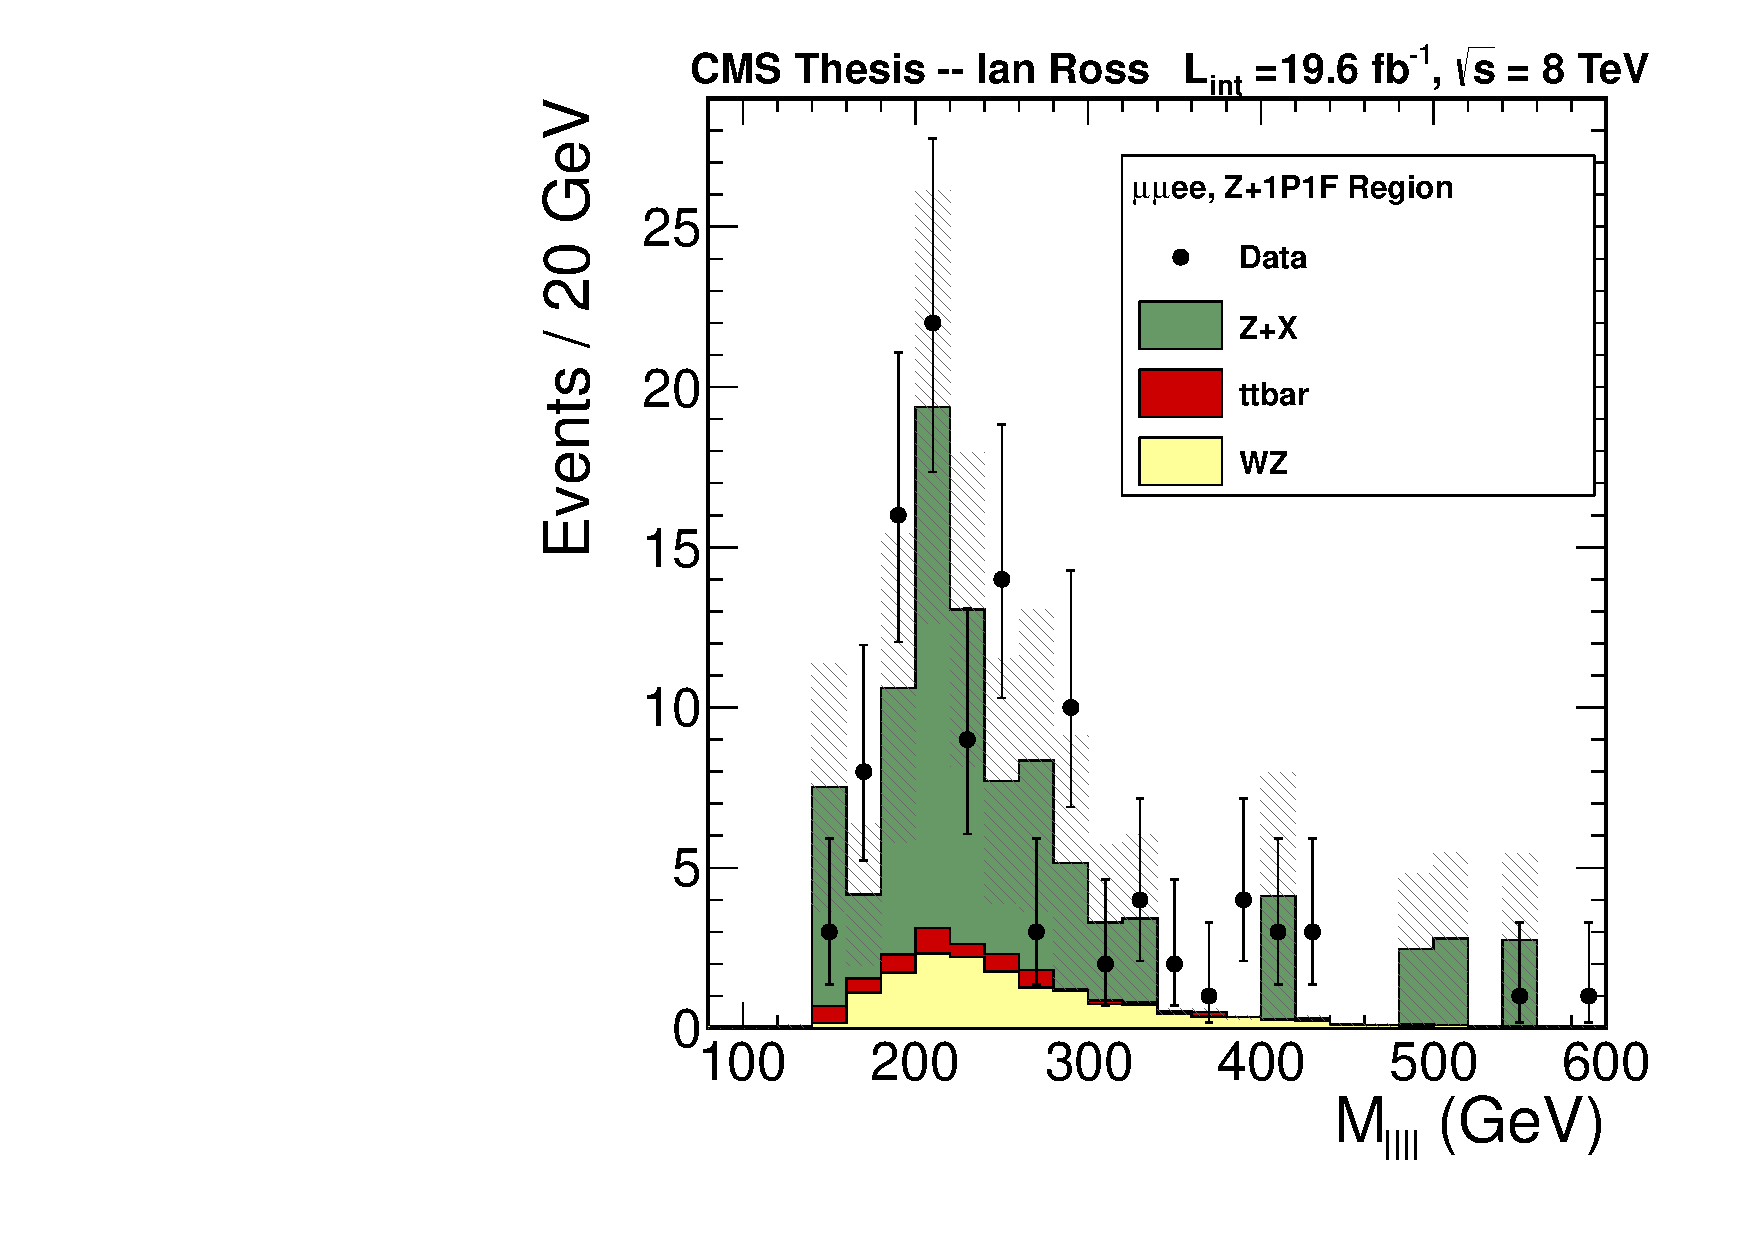
\includegraphics[width=0.45\textwidth]{mmee_IA_highmass}\\
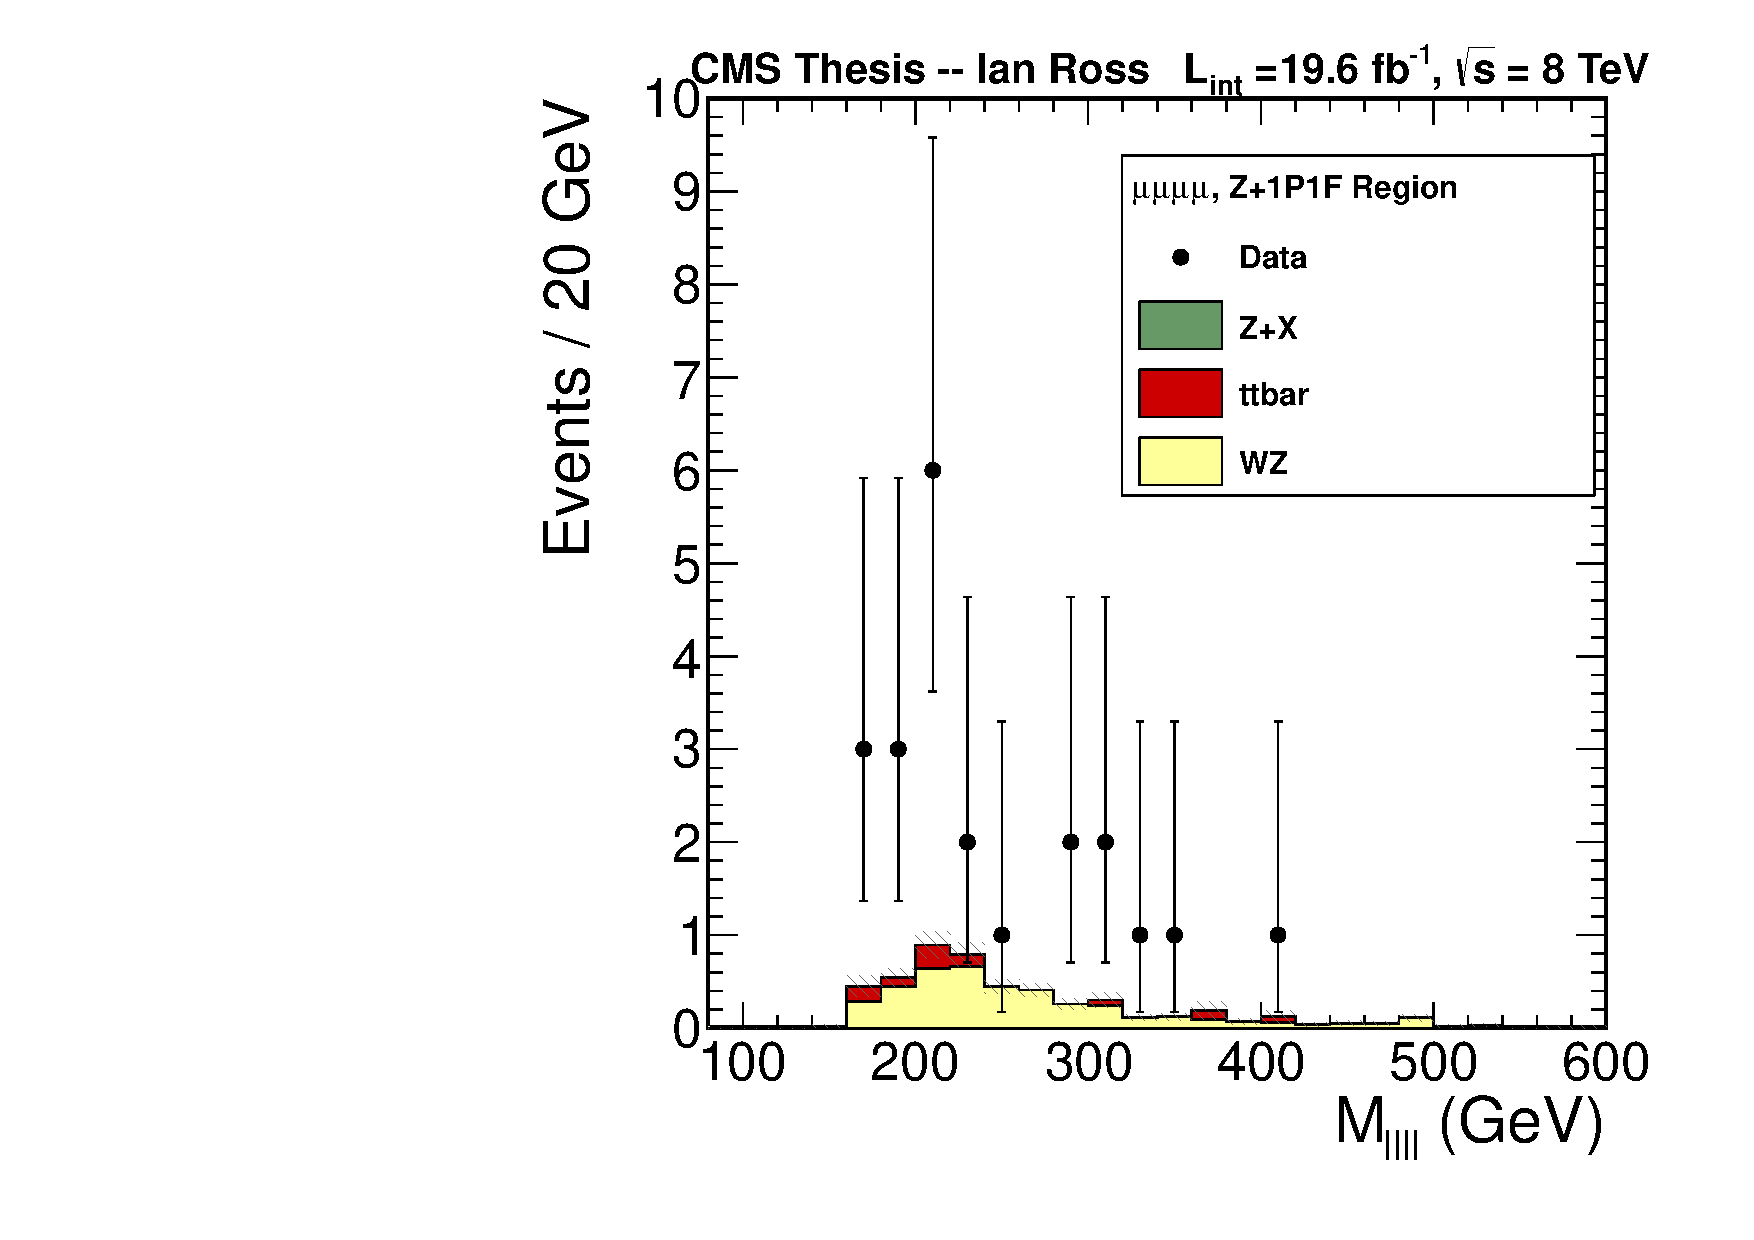
\includegraphics[width=0.45\textwidth]{mmmm_IA_highmass}
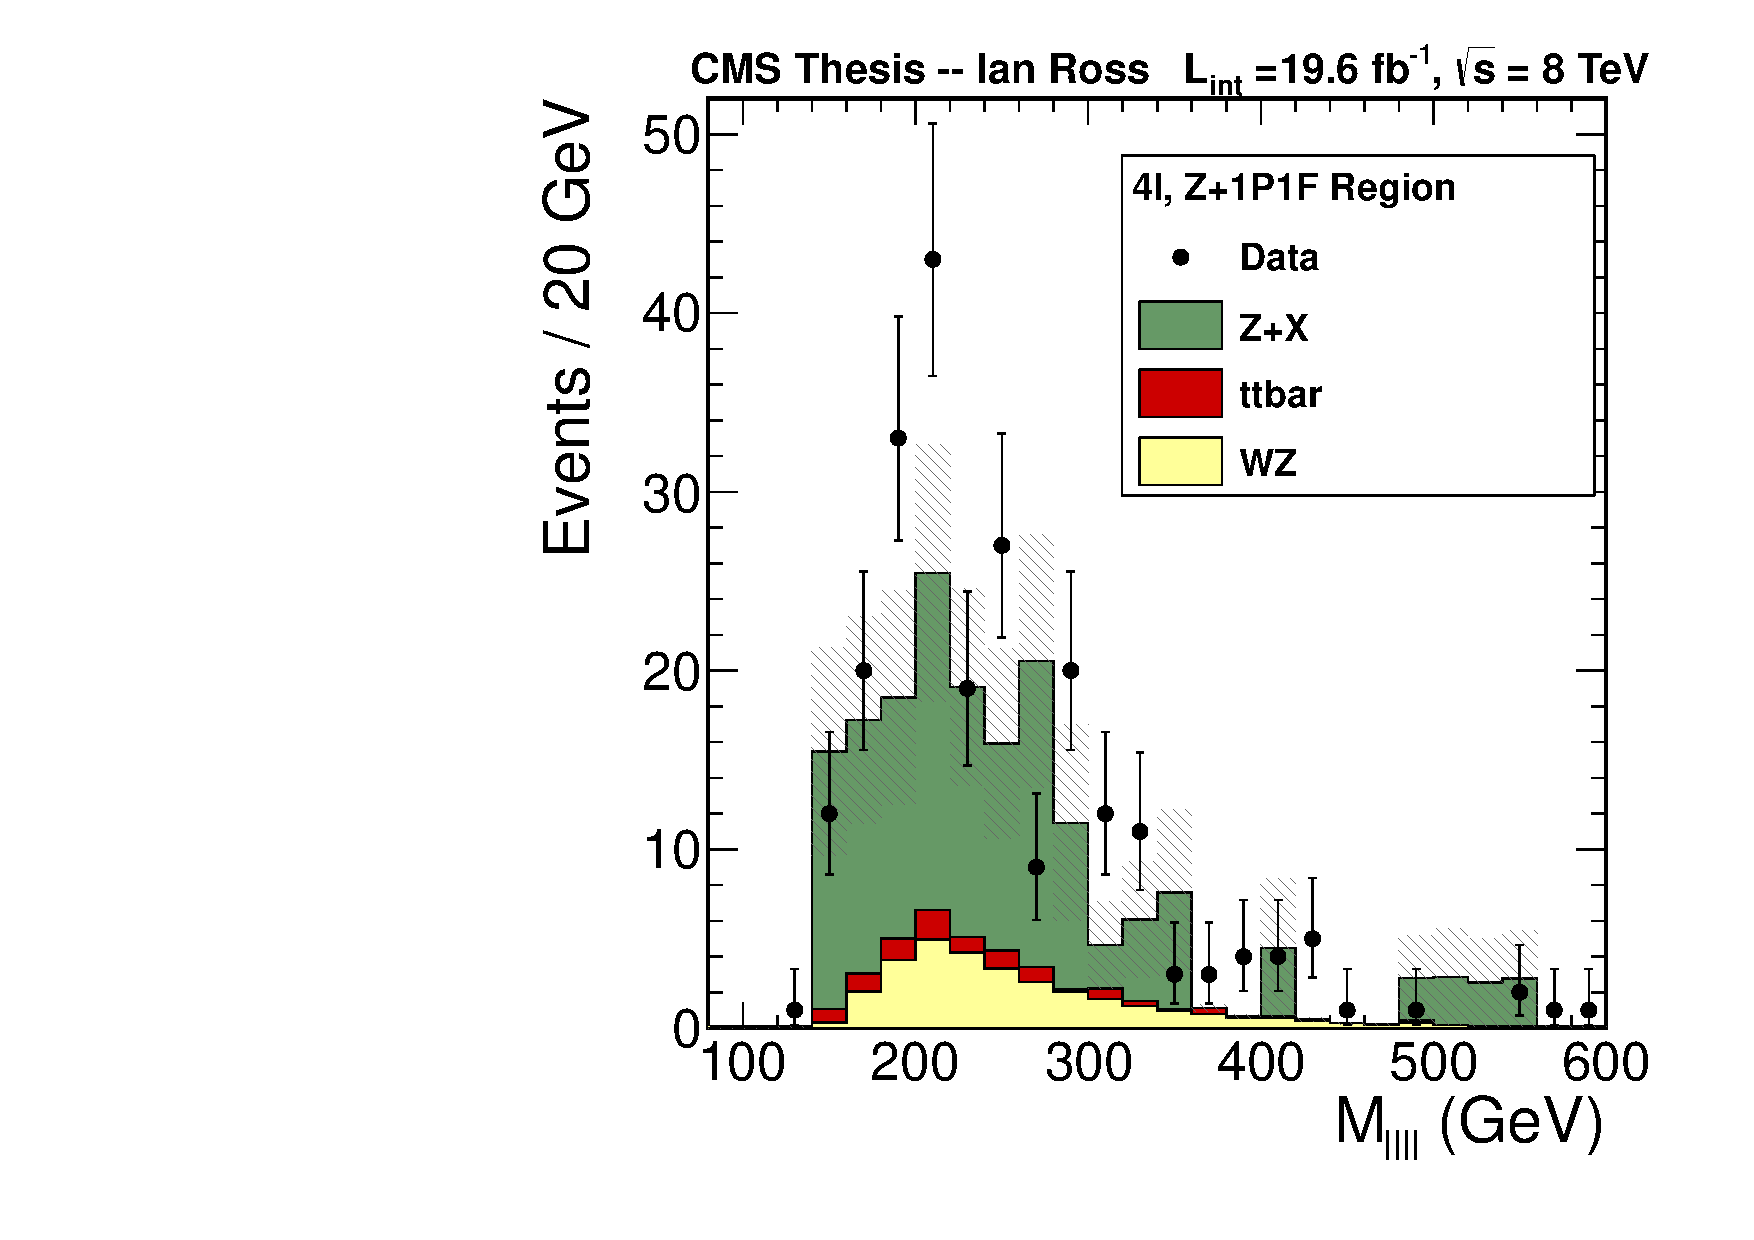
\includegraphics[width=0.45\textwidth]{4l_IA_highmass}\\
\caption[Background estimation region consisting of a \Z plus one passed and one failed
leptons, with the high mass requirement.]{Background estimation region consisting of a \Z plus one passed and
    one failed leptons, with the high mass requirement. Counter clockwise from top right is the eeee, $\mu\mu
    ee$, $\mu\mu\mu\mu$, and summed final states.}
\label{fig:AIregions_highmass}
\end{figure}


In general, $N_F$ background-like events fail the final selection while $N_P$
background-like events pass the final selection, and the fake rate can be written as
\begin{equation}
    f = \frac{N_P}{N_P+N_F} 
\end{equation}
As a result, the population of background events passing the signal selection
can be written as:
\begin{equation}
    \label{eqn:np}
    N_P = N_F \frac{f}{1-f}
\end{equation}

If one assumes the fake rates of Equations~\ref{eqn:fr} and~\ref{eqn:np} are the
same, then the final background is estimated by applying the measured fake rate to
the regions as follows:
\begin{equation*}
    \textrm{Estimated Background} = \frac{f}{1-f}
    N_{\textrm{1P1F}} - \frac{f^2}{(1-f)^2} N_{\textrm{2F}}
\end{equation*}
where $N_{\textrm{1P1F}}$ is the number of events in the Z+1P1F region, with the
MC-driven expectation of ZZ contamination removed and $N_{\textrm{2F}}$ is the
Z+2F equivalent. The removal of the Z+2F contribution is required due to the
fact that these events are doubly represented in the Z+1P1F region, as the
population here already contains Z+2jet events that underwent a $2 \choose 1$
migration, as there are two selected lepton `slots' for a jet to fake. The flow
of these events is diagrammed in~\ref{fig:bgFlow}. 

\begin{figure}[h]
\centering
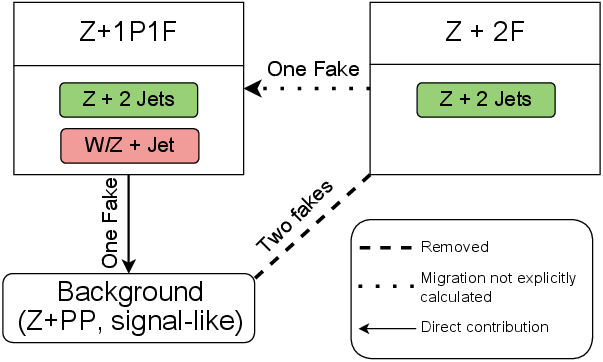
\includegraphics[width=0.80\textwidth]{bgFlow2Cat}
\caption[Diagram depicting the flow of events in the reducible background
estimate.]{Diagram depicting the flow of events in the reducible background. A
dotted line indicated a migration that does not explicitly enter the background
estimate, a solid line indicates a positive net contribution, while a dashed
line indicates a removal from the estimate. The ``P'' and ``F'' stand for
additional loose leptons which pass or fail final selections, respectively.}
\label{fig:bgFlow}
\end{figure}

\section{Final State Radiation Recovery}
It is possible for electrons and muons produced in a Z boson decay to radiate a
photon, resulting in a $Z\rightarrow \ell \ell \gamma$ final state. Because the
photons are emitted along an almost equal trajectory, the electron
reconstruction process often captures these additional photons. However, it is
possible that the electron reconstruction misses the radiated photons and, in
addition, no such recovery is inherent to the muons. Given the criticality of
precise mass measurements, a final state radiation (FSR) recovery algorithm is
implemented in order to fully reconstruct the four-momentum of the Z candidates. 

The FSR recovery begins by first defining a set of FSR-candidate photons. To
start, a collection of photons is built from the Particle Flow photon
collection. In addition, photon candidates are built from the electromagnetic
calorimeter deposits near Particle Flow muons. The photons are required to have
$p_T > 2$~GeV, within $|\eta|$ of 2.4, and be well separated from the
superclusters of any electrons passing the $p_T$, identification, and vertex
compatibility requirements ($\Delta R > 0.15$, $\Delta \phi > 2$, and $\Delta
\eta > 0.05$).  The isolation for these photons is then computed, using a cone
size of $\Delta R < 0.3$, with thresholds of 0.2 and 0.5~GeV on the charged and
neutral+photon components. 

For each photon, the nearest lepton from the Z candidate is found. If the photon
is co-linear with the lepton ($\Delta R(\ell \gamma) < 0.015$, then the photon is
kept. If the separation between the photon and lepton is wider ($\Delta R(\ell
\gamma) < 0.5$), then the photon is kept if its $p_T$ is above 4~GeV and its
relative isolation is less than 1.

Finally, the list of FSR candidate photons is considered with the Z candidate
objects.  It is important to note that these Z candidates are built from leptons
with the isolation criteria not yet applied, as the FSR photon's removal from
the leptons' isolation can cause them to migrate from failing to passing the
selection.  With the four-momenta of the photon summed to that of the Z
candidate, the photon is considered to be a successful recovery if:
\begin{itemize}
    \item $| M_{\ell \ell \gamma} - M_{\Z} | < | M_{\ell \ell} - M_{\Z} | $
    \item $4 < M_{\ell \ell \gamma} < 100~GeV$
\end{itemize}
If these criteria are met, then the photon is removed from that Z candidate's
leptons' isolation cones and the Z ($\rightarrow \ell \ell \gamma$) object is
considered to as the Z candidate.

The effects of the FSR recovery can be seen on simulated $\Z \rightarrow ee$ and $\Z
\rightarrow \mu \mu$ peaks in Figure~\ref{fig:fsrRecovery}. 

\begin{figure}[h]
\centering
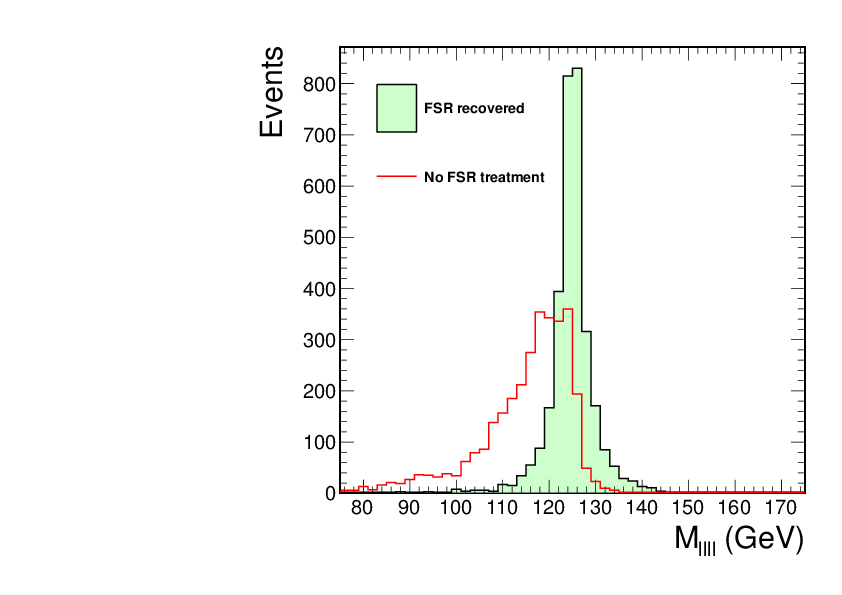
\includegraphics[width=0.50\textwidth]{recovered_fsr}
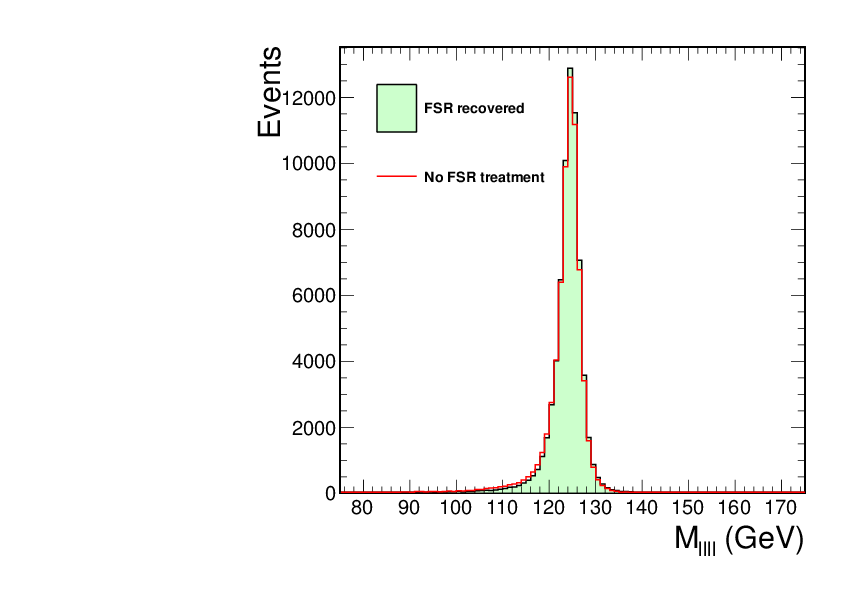
\includegraphics[width=0.50\textwidth]{recovered_fsr_all}
\caption[A simulated $H\rightarrow2e2\mu$ ($m_H = 125 GeV$) peak, with and without FSR
recovery.]{A simulated $H\rightarrow2e2\mu$ ($m_H = 125 GeV$) peak, with and without the
    FSR recovery. The FSR recover effects only a fraction (~6\% total, top) of the
    events, but the overall effect (bottom) is a few percent gain in resolution.
}
\label{fig:fsrRecovery}
\end{figure}

\section{Kinematic Discriminant}
A kinematic discriminant is introduced in order to utilize the angular
differences between $H\rightarrow ZZ \rightarrow \ell\ell\ell\ell$ and $ZZ
\rightarrow \ell\ell\ell\ell$ decays. Five angles define the angular system in
the ZZ rest frame (as pictured in diagram~\ref{fig:angles}:
\begin{itemize}
    \item $\theta_1$ and $\theta_2$, the helicity angles defined in each Z's
        rest frame.
    \item $\theta\ast$, the production angle of the Z boson with respect to the
        beam axis
    \item $\Phi_1$, the azimuthal angle between the Z1 decay plane and the Z
        production plane
    \item $\Phi$, the angle between the Z1 and Z2 decay planes
\end{itemize}

The probability that a Higgs (or ZZ) candidate was created with invariant Z
masses $M_{Z1}$ and $M_{Z2}$ and an angular system defined by the angles $\vec
\Omega$ are proportional to their respective elements:
\begin{equation}
    P_{signal} (M_{Z1}, M_{Z2}, \vec \Omega | M_{\ell\ell\ell\ell} ) = |
    ME_{signal} |^2
\end{equation}
\begin{equation}
    P_{bkg} (M_{Z1}, M_{Z2}, \vec \Omega | M_{\ell\ell\ell\ell} ) = |
    ME_{bkg} |^2
\end{equation}
A kinematic discriminant can be built to classify events as more or less
signal-like:
\begin{equation}
    KD = \frac{P_{signal}}{P_{signal}+c\cdot P_{bkg}} = \left(1+\frac{c\cdot
    P_{bkg}}{P_{signal}} \right)^{-1}
\end{equation}
This gives a continuously varying discriminant, with background-like events
pushed toward 0 and signal-like events near 1.
$P_{bkg}$ is evaluated using MCFM~\cite{MCFM}, while JHUGen~\cite{spin} is used to train
the signal samples.

\begin{figure}[h]
\centering
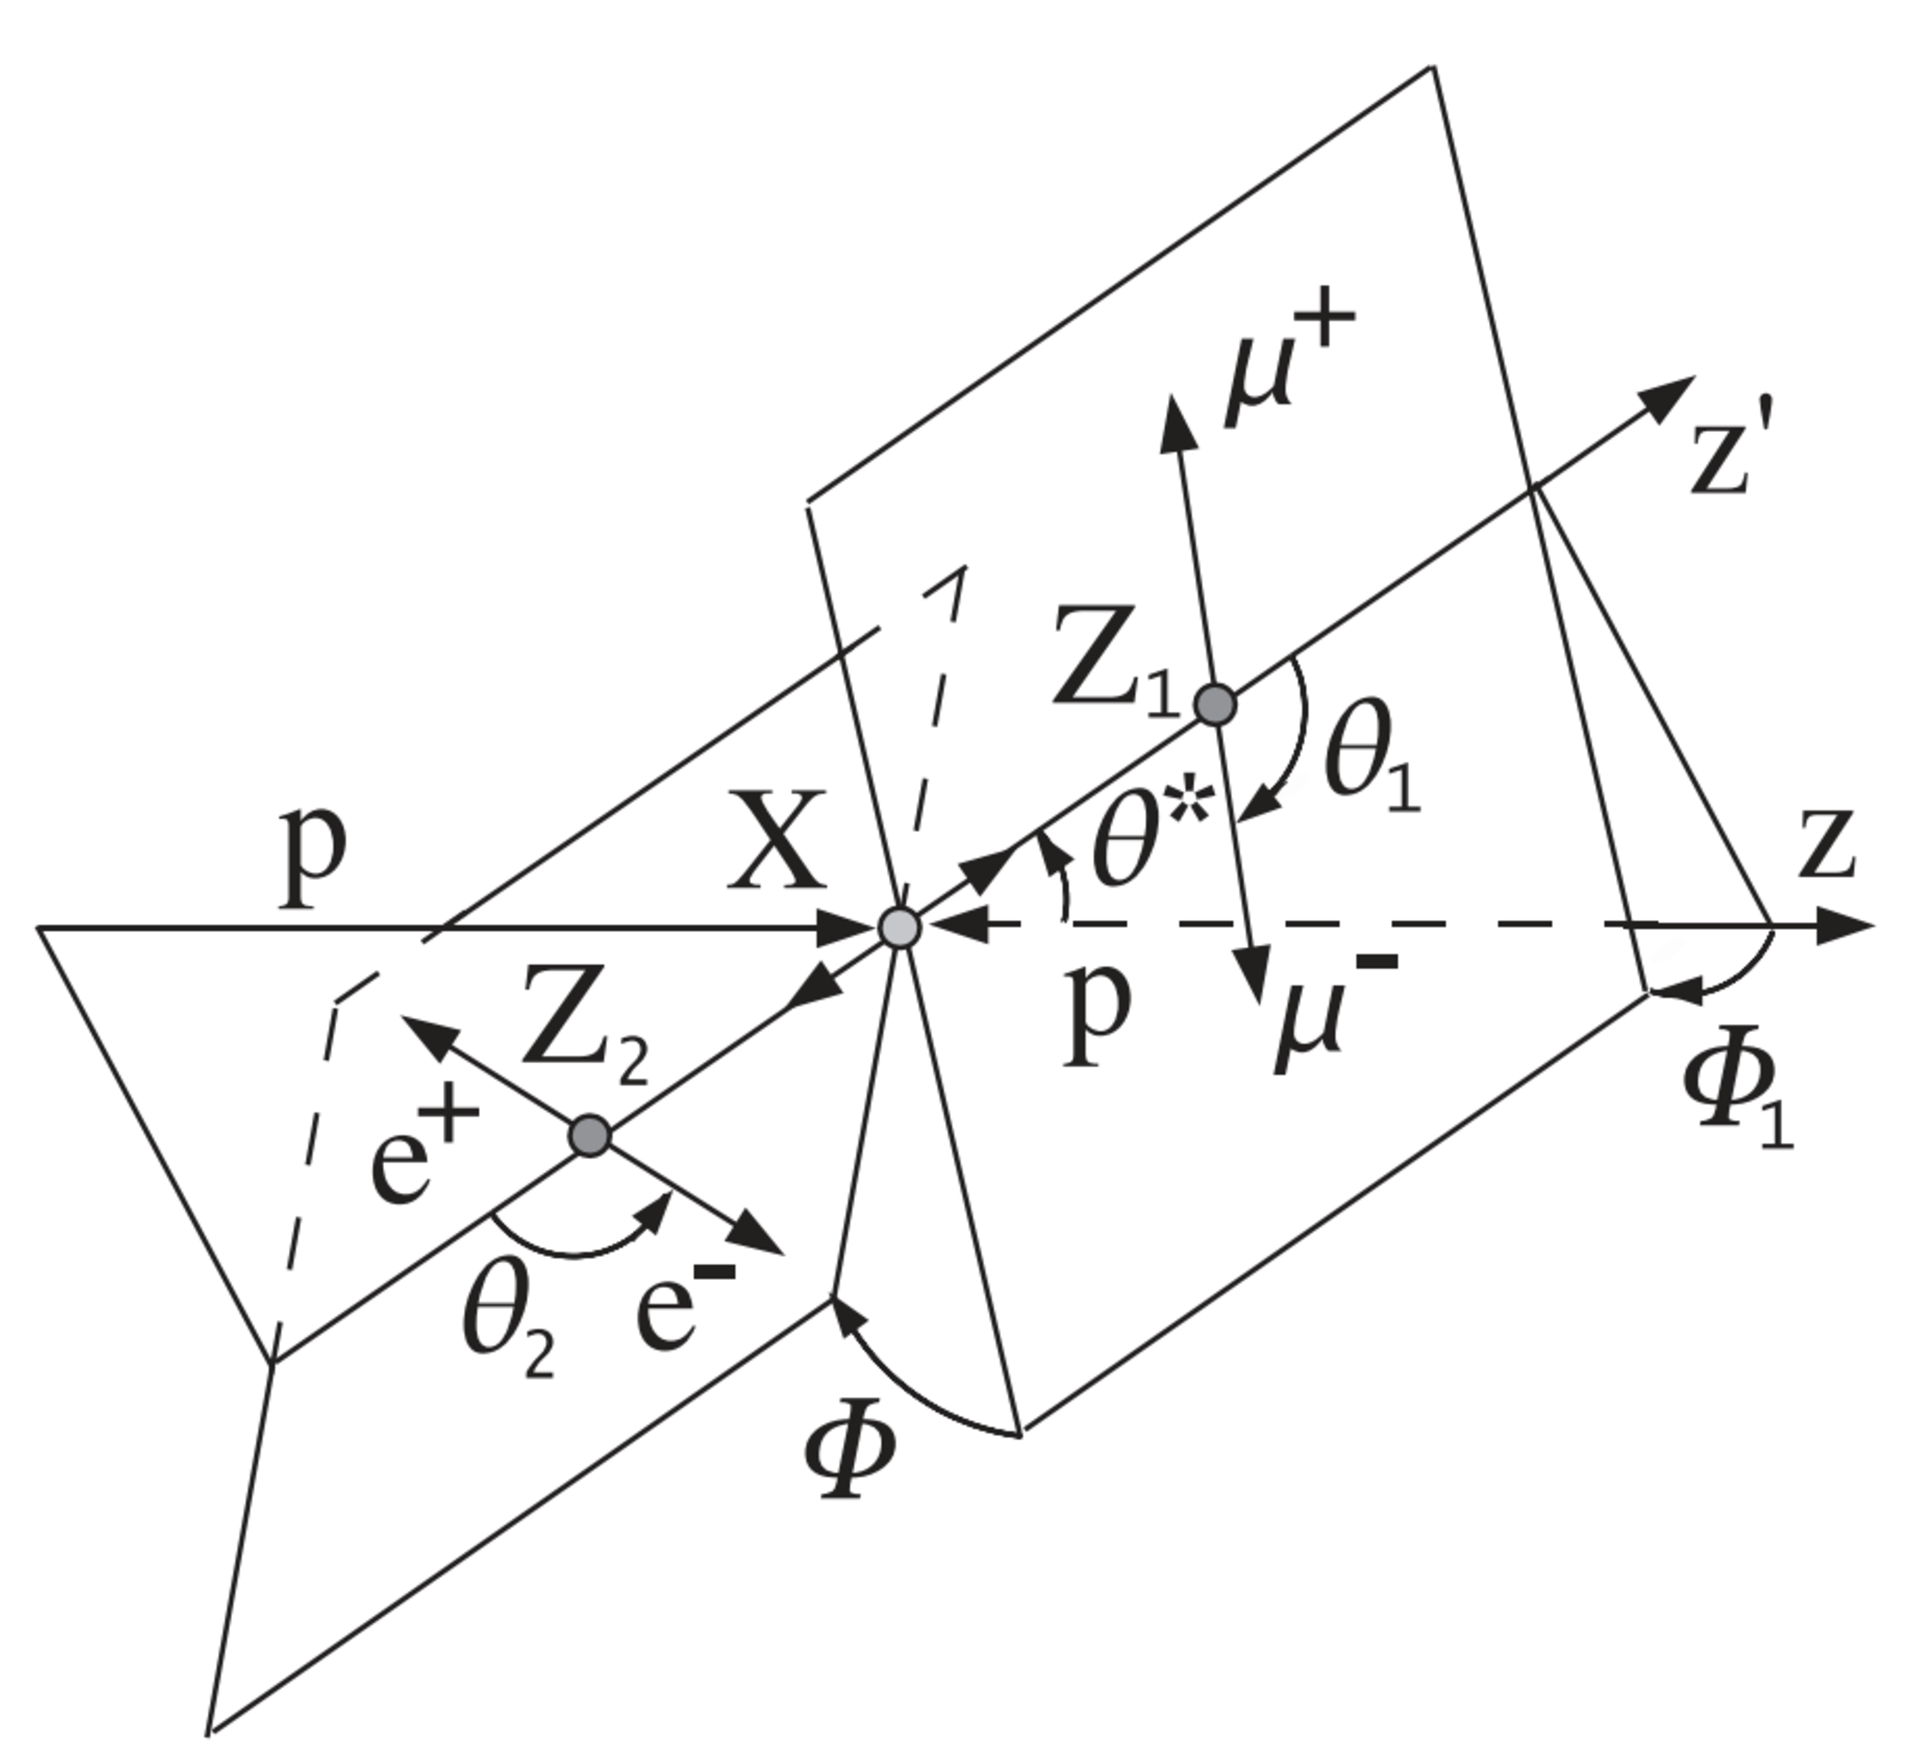
\includegraphics[width=0.60\textwidth]{angles}
\caption[The angular definitions in the ZZ rest frame.]{The angular definitions
in the ZZ rest frame.}
\label{fig:angles}
\end{figure}

\section{Final event selection}
In order to build the final physics events, the selected leptons must be
combined into composite Z candidates, which in term are combined into the final
ZZ system. This is done by first combining same-flavor (SF), opposite sign leptons
(which pass all identification criteria) into an initial Z candidate. Then the
remaining leptons (which pass the loose criteria defined above) are combined
into same-flavor combinations. All possible combinations of Z candidate plus SF
combinations are stored from the events, allowing easy access to both
signal-like events (in which the second candidate passes the tighter criteria
are are of opposite sign) and background-like events (in which the second pair
of leptons fail the tighter selection and/or are of the same sign). 

For both of these sets of Z candidates (both those explicitly passing
identification and those that have no restrictions), the FSR recovery is run.
This allows the effects of the FSR state recovery to be properly accounted for
in both signal and background-like candidates. 

After the FSR recovery, the isolation requirements are placed onto the first Z
candidate. Then, selection criteria are applied onto the second Z candidate,
sorting the ZZ candidates into signal, Z+1P1F, or Z+2F regions (for both SS and OS
secondary pairs).

\subsection{Candidate combinatorics and arbitration}
In the $eeee$ and $\mu\mu\mu\mu$ final states, the ways in which to
combine the opposite-sign, same flavor pairs is ambiguous. Additionally, it is
possible that more than four good leptons exist, allowing multiple ZZ candidates
to exist within an event. 
This effect, plus the asymmetric mass selections, on the Z candidates means that
some arbitration must be applied. The simplest arbitration is the ``best Z
mass'' selection, in which the $Z_1$ is defined to be the pair whose invariant
mass is closest to the nominal Z mass. Then, from the remaining possible $Z_2$
candidates, the one with the highest scalar sum of lepton $p_T$s is chosen.

The background regions are treated differently. Because each of the candidates
represents a possible migration into the signal region, all unique combinations
are kept. 

\subsection{Signal selection}
This analysis considers two separate set of criteria in its two separate
searches. The two criteria differ only in the criteria placed on the invariant
masses of the Z candidates.
The Higgs search necessitates picking up $Z\gamma*$ contributions, so a wider
invariant mass range is allowed:
\begin{equation*}
40 < M_{Z_1} < 120 GeV
\end{equation*}
\begin{equation}
12 < M_{Z_2} < 120 GeV
\label{eqn:lowmass}
\end{equation}

In the measurements pertaining to the anomalous triple gauge couplings and
ZZ differential cross sections, both \Z bosons are required to be on-shell,
eliminating the contributions from $\gamma *$ production:

\begin{equation*}
60 < M_{Z_1} < 120 GeV
\end{equation*}
\begin{equation}
60 < M_{Z_2} < 120 GeV
\label{eqn:highmass}
\end{equation}
The Higgs search (the so-called low-mass criteria) and the Standard Model/triple
gauge coupling measurements (the high-mass criteria) differ only in the mass
requirements listed in equations~\ref{eqn:lowmass} and~\ref{eqn:highmass}.

\begin{figure}[h]
\centering
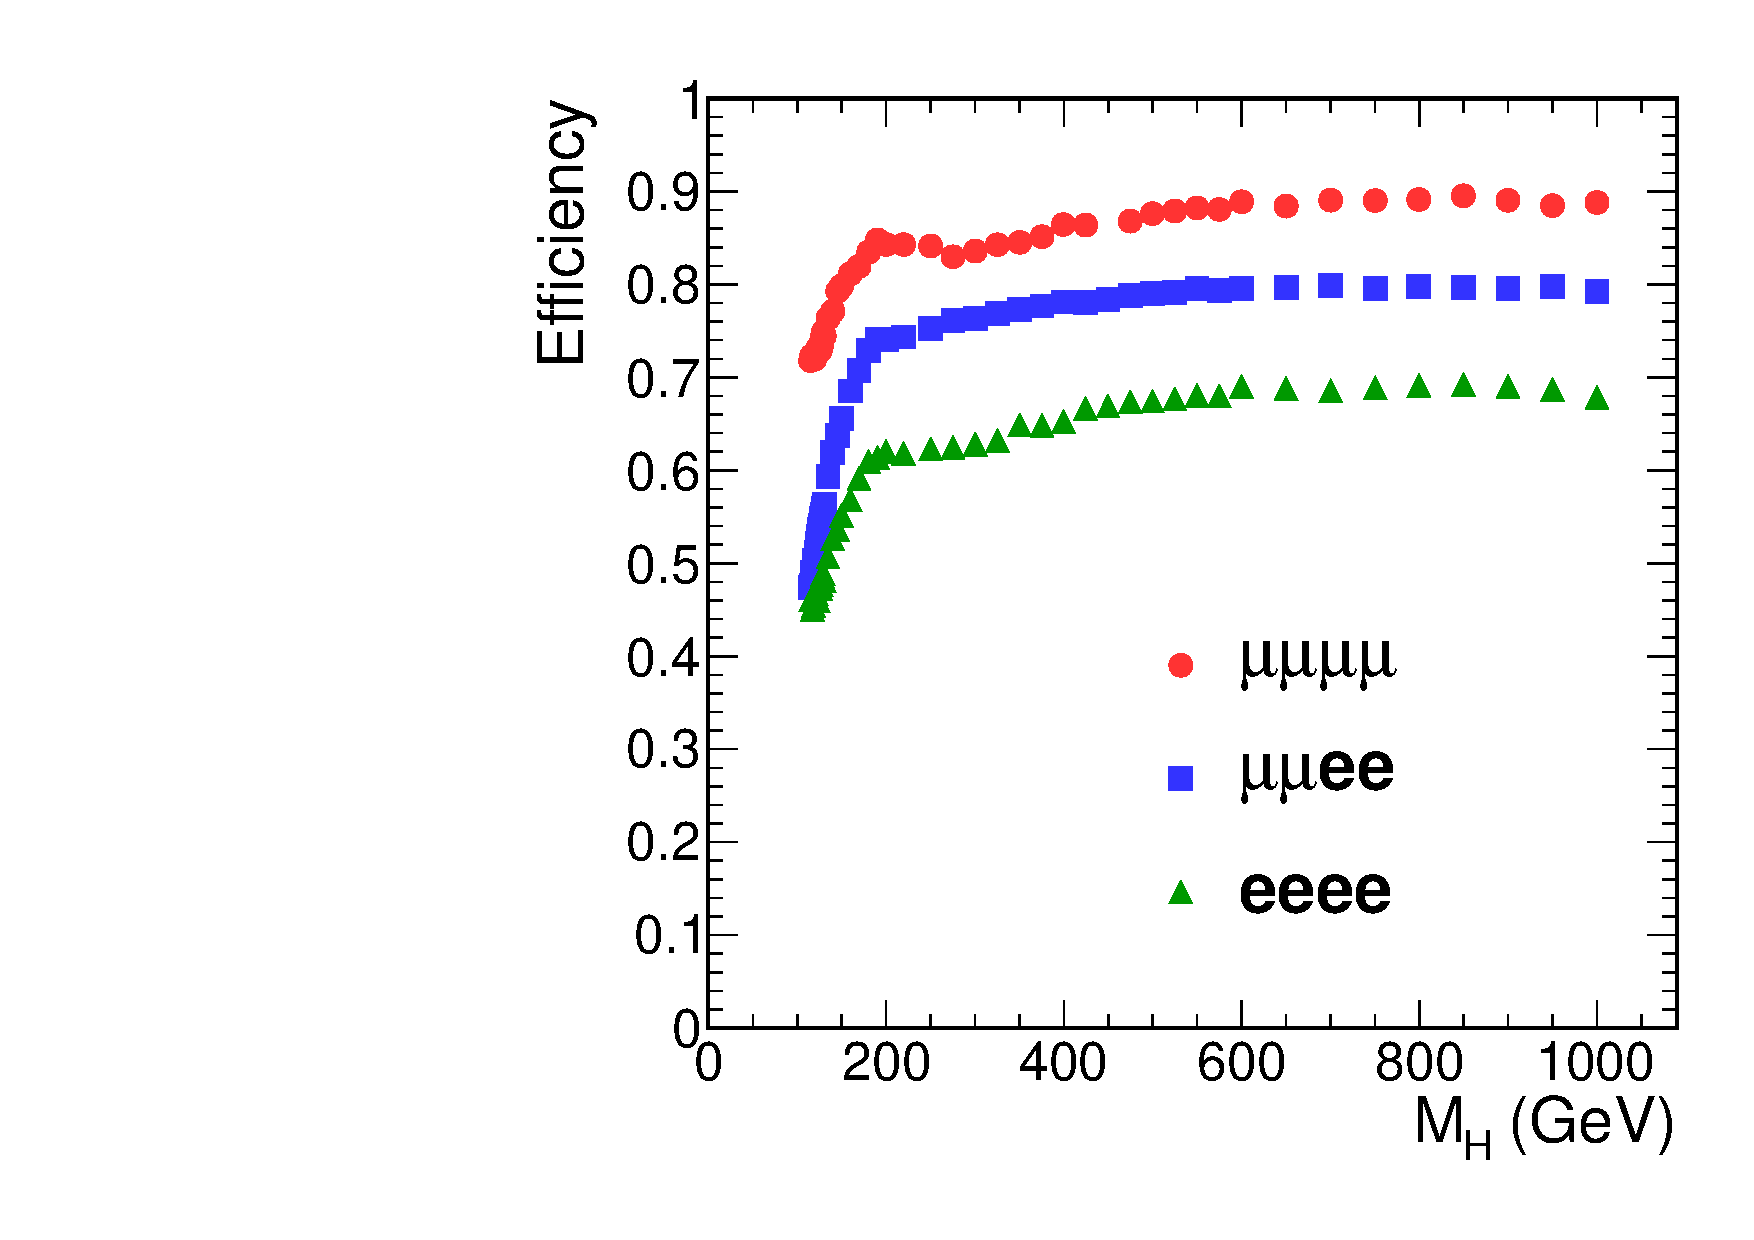
\includegraphics[width=0.80\textwidth]{higgs_eff}
\caption[Final selection efficiency, as a function of Higgs mass.]{Final selection efficiency for each final
state, as a function of the Higgs mass. Efficiency is defined as the number of
selected events to the number of events produced within the geometrical and
kinematic requirements of the analysis.}
\label{fig:selEff}
\end{figure}



%\section{Acceptance}
\section{Signal and background modelling}

In the search for a Standard Model Higgs boson, the differential distribution
(with respect to the four-lepton invariant mass) is factorized as:
\begin{equation}
    \label{eqn:higgsShape}
    \frac{dN}{dM_{\ell\ell\ell\ell}} = C_{\epsilon} \cdot N^{MC}(m_H)
    \cdot F_H(M_{\ell\ell\ell\ell} | m_H)
\end{equation}
where $C_\epsilon$ is the product of the leptonic correction factors (described
in section~\ref{sub:scale_factors}), $m_H$ is the hypothesized Higgs boson mass,
and $F_H$ is the probability density function of the Higgs mass distribution.
This function is a convolution of a relativistic Breit-Wigner
function~\footnote{$\frac{\Gamma_{gg}(m_{4\ell})\cdot\Gamma_ZZ(m_{4\ell})\cdot m_{4\ell}}
{(m_{4\ell}^2-m_{H}^2)^2+m_{4\ell}^2\cdot\Gamma^2(m_{4\ell})}$} with a
double Crystal Ball function~\footnote{$\begin{cases} 
A \cdot (B+|\xi|)^{-n_L} &\text{for } \xi < \alpha_L \\ 
A \cdot (B+|\xi|)^{-n_R} &\text{for } \xi > \alpha_R \\ 
exp(-\xi^2/2), & \text{for } \alpha_L \le \xi \le \alpha_R  \\
\xi = (m_{4\ell} - m_{H} - \Delta m_{H} )/ \sigma_m
\end{cases}$}, added to account for the low- and high-side tails
from bremsstrahlung effects and detector mismeasurement effects.
The shape parameters are fit using the available Monte Carlo simulation samples,
then a secondary fit to the shape parameters is used in extracting shape values
between the generated samples. This allows a smoothly varying shape to be used
as input across an arbitrary Higgs mass hypothesis range.
A full description of the shape and its parameters is given
in~\cite{higgsSigShape}.

For a low ($< 400~GeV$) mass Higgs hypothesis, the implicit zero-width
assumption used in the fitting procedure above holds valid. However, as the
Higgs width becomes wider, this assumption breaks down. As a result, all cross
sections and lineshapes in the high-mass Higgs hypotheses utilize the
\emph{Complex Pole Scheme (CPS)}~\cite{higgsLineshape}. Additionally,
interference between Higgs and $gg\rightarrow ZZ$ production causes a significant
deformation in the invariant mass distribution. This is corrected (and
uncertainties computed) using the scheme proposed in
~\cite{higgsHighMassInterference}. The uncertainties are explained in
Section~\ref{sec:systematics}.

In the Higgs search, the ZZ background is treated in a way similar to the Higgs
signal (Eqn.\ref{eqn:higgsShape}). However the shape, $F_H$, is replaced by:

\begin{equation*}
    \frac{dN_{qq\rightarrow ZZ}}{dM_{\ell\ell\ell\ell}} = C_{\epsilon} \cdot N^{MC}(m_H)
        \cdot ( f_1 + f_2 + f_3 )
\end{equation*}
\begin{equation*}
    \frac{dN_{gg\rightarrow ZZ}}{dM_{\ell\ell\ell\ell}} = C_{\epsilon} \cdot N^{MC}(m_H)
        \cdot ( f_1 + f_2 )
\end{equation*}
\begin{equation*}
    f_1(m, \vec{a}) = \left(0.5 + 0.5
        erf(\frac{m-a_1}{a_2}) \right ) \cdot \frac{a_4}{1+\exp{(m-a_1)/a_3}}
\end{equation*}
\begin{equation*}
    f_2(m, \vec{b}) = \left(0.5 + 0.5
        erf(\frac{m-b_1}{b_2}) \right ) \cdot \left (
        \frac{b_4}{1+\exp{(m-b_1)/b_3}} + \frac{b_6}{1+\exp{(m-b_1)/b_5}}
        \right)
\end{equation*}
\begin{equation}
    f_3(m, \vec{c}) = \left(0.5 + 0.5
        erf(\frac{m-c_1}{c_2}) \right ) \cdot \frac{c_4}{1+\exp{(m-c_1)/c_3}}
\end{equation}

\section{Systematic Uncertainties}
\label{sec:systematics}

\subsection{Higgs Signal Simulation}
Systematic uncertainties for the Higgs samples effect either the overall
yield or the shape of the signal. Uncertainties that enter only through the
yield include:
\begin{itemize}
\item Uncertainty on Higgs production cross section, $H\rightarrow ZZ$, and
    $ZZ\rightarrow 4\ell$ branching ratios.
\item Uncertainty on acceptance measurements
\item Uncertainties on data-to-MC correction factors
\end{itemize}
while uncertainties that impact the signal shape are:
\begin{itemize}
    \item The theoretical uncertainties in the pdf of the Higgs shape, $F_H(M_{\ell\ell\ell\ell} | m_H)$
    \item Uncertainties in the modelling of detector effects within the double
        Crystal ball fit
\end{itemize}

The uncertainty on the Higgs production cross section arises from the PDF and
$\alpha_s$ (the strong force coupling strength) errors in addition to
uncertainties in the QCD renormalization ($\mu_R$)  and 
factorization ($\mu_F$) scales (which are theoretical constructs to remove
divergent cross section calculations).
These values, in addition to the cross sections themselves, are provided by the
LHC working group~\cite{lhcHiggsHandbook}.  Effects due to the acceptance are
measured using MCFM, adjusting $\mu_R$ and $\mu_F$ up and down by a factor of
two and calculating the total change in acceptance. These uncertainties are
found to be at the 0.1-0.2\% level, and are neglected. PDF and $\alpha_s$
effects on the acceptance are measured using the PDF4LHC
prescription~\cite{PDF4LHC}, in which three different PDF sets are used
(\cite{ct10}, \cite{MSTW08}, \cite{nnPDF}), with the maximum differences being
the final systematic effect. This is found to be a fairly flat effect across all
Higgs masses, and a flat 2\% systematic is applied.

Shape systematic uncertainties are measured by utilizing alternate shape
hypotheses, refitting the samples, and taking the envelope of the outcomes as
the systematic error.

The data-to-MC scale factors corrections, obtained from the tag and probe method
outlined in Section~\ref{sub:scale_factors}, are applied on a per-lepton basis.
Each lepton provides an additional weight factor that is applied when extracting
the Monte Carlo yield. Uncertainties in the correction factor measurements
(coming from shape and modelling uncertainties in the tag and probe process) are
propagated into a final uncertainty by running, for each MC sample, a batch of
500 toy MC experiments. For each, the correction factor is extracted via a
Gaussian, centered at the data/MC ratio and with a $\sigma$ equal to the
associated error. The final systematic uncertainty on the MC yields is defined
to be the RMS of the distribution of these pseudoexperiments.


\subsection{ZZ Simulation}
Many of the systematic uncertainties on ZZ are similar to those for the Higgs signal.
Uncertainties on the total yields are due primarily to the theoretical
uncertainties, PDF+$\alpha_s$ and QCD scales, and the instrumental uncertainties
on the data-MC scaling.

PDF+$\alpha_s$ uncertainties are again evaluated using the PDF4LHC method, as
with the Higgs sample. The $qq \rightarrow ZZ$ and $gg\rightarrow ZZ$
errors are evaluated separately, and vary roughly with the square root of the
$M_{\ell\ell\ell\ell}$:
\begin{equation*}
    qq\rightarrow ZZ : \kappa (M_{\ell\ell\ell\ell}) = 1 + 0.0035
    \sqrt{M_{\ell\ell\ell\ell} - 30}
\end{equation*}
\begin{equation}
    gg\rightarrow ZZ : \kappa (M_{\ell\ell\ell\ell}) = 1 + 0.0066
    \sqrt{M_{\ell\ell\ell\ell} - 10}
\end{equation}

QCD scale uncertainties are treated the same way, measuring the envelope of errors
resulting from scaling $\mu_F$ and $\mu_R$, with uncertainties
parameterized as:
\begin{equation*}
    qq\rightarrow ZZ : \kappa (M_{\ell\ell\ell\ell}) = 1.00 + 0.01\sqrt{(M_{\ell
    \ell\ell\ell} -20)/13}
\end{equation*}
\begin{equation*}
    gg\rightarrow ZZ : \kappa (M_{\ell\ell\ell\ell}) = 1.04 + 0.10\sqrt{(M_{\ell
    \ell\ell\ell} +40)/40}
\end{equation*}

\subsection{Systematic Uncertainties on Reducible Backgrounds}
The uncertainties on the reducible background estimates come primarily from the
limited statistics in the regions where fake rates are applied, the
uncertainties in the measured fake rates, and the uncertainty in the
difference in background sources while migrating between the regions. MC closure
tests and OS/SS checks were conducted, but were limited by statistics. Alternate
reducible BG calculations were conducted, and a conservative estimate of 30-50\%
was applied (depending on the final state).

\subsection{Global Uncertainties in MC-driven estimates}
In addition to the uncertainties outlined above, there are two global effects
which impact the yield extraction from the Monte Carlo simulated samples. First,
uncertainties in the measurement in the integrated luminosity were found to be
4.4\%~\cite{lumi}. Additionally, the uncertainty on the trigger corrections (which come from
tag and probe measurements) is evaluated to 1.5\%~\cite{zzHiggsMoriond}.

\section{Summary}
The selection criteria for the search of a $ZZ\rightarrow \ell\ell\ell\ell$
final state is designed to be as loose as possible in order to maximize the
efficiency of this clean, though low-probability, final state. The final
selection criteria on electrons, muons, and Z boson candidates are summarized in
Table~\ref{tab:selection_criteria}.

\begin{table}[h]
\centering
\begin{tabular}{|c|c|}
\hline
\multicolumn{2}{|c|}{Electron selection} \\
\hline
Kinematics & $p_T > 7~GeV$, $|\eta| < 2.5$ \\
Identification & MVA ID as defined above. \\ 
Isolation & $rho$-corrected relative isolation < 0.40 \\
\hline
\multicolumn{2}{|c|}{Muon selection} \\
\hline
Kinematics & $p_T > 5~GeV$, $|\eta| < 2.4$ \\
Identification & (Global OR Tracker), PF Muon \\
Isolation & $rho$-corrected relative isolation < 0.40 \\
\hline
\multicolumn{2}{|c|}{Z Candidate Selections} \\
\hline
Higgs search (low-mass) & $40 < M_{Z1} < 120~GeV$ \\
                        & $12 < M_{Z2} < 120~GeV$ \\
SM ZZ and aTGC analysis (high-mass) & $60 < M_{Z1} < 120~GeV$ \\
                        & $60 < M_{Z2} < 120~GeV$ \\
\hline
\end{tabular}
\caption[Summary of the selection criteria.]{Summary of the selection criteria.}
\label{tab:selection_criteria}
\end{table}

Additionally, careful consideration of systematic uncertainties, both on
expected yields and shapes of signals and background, have been evaluated. These
uncertainties are summarized in Table~\ref{tab:systematics}.

\begin{table}[h]
\small
\centering
\begin{tabular}{|c|c|c|c|c|c||c|c|}
    \hline
    & ggH & VBF & WH & ZH & ttH & $qqZZ$ & $ggZZ$ \\
    \hline
    $gg$ pdf uncertainty & 7.2-9.2 & - & - & - & 0-9.8 & - & 10 \\
    $qq / q\overline q$ pdf uncertainty & - & 1.2-1.8 & 0-4.5 & 0-5.0 & - & 5 &
    - \\
    QCD Scale & 5.5-7.9 & 0.1-0.2 & 0-0.6 & 9-1.5 & 0-8.8 & 2.6-6.7 & 24-44 \\
    $H\rightarrow 4l$ BR & 2 & 2 & 2 & 2 & 2 & - & - \\
    \hline
    CB mean parameterization  & \multicolumn{5}{c||}{0.4} & - & - \\
    CB $\sigma$ parameterization & \multicolumn{5}{c||}{ 20 } & - & - \\
    CB $\alpha$ parameterization & \multicolumn{5}{c||}{ 20 } & - & - \\
    \hline
    Luminosity & \multicolumn{7}{c|}{ 4.2 } \\ 
    Trigger & \multicolumn{7}{c|}{ 1.5 } \\
    Electron efficiency scale & \multicolumn{7}{c|}{ 6.2-11} \\
    Muon efficiency scale & \multicolumn{7}{c|} { 1.9 } \\
\hline
\end{tabular}
\caption[Summary of the systematic uncertainties.]{Summary of the systematic
uncertainties.}
\label{tab:systematics}
\end{table}


\chapter{Results}
\label{chapter:results}
%%%%

The analysis presented in this analysis is split into two selection criteria,
differing only by an on-shell ($60 < M_{Z} < 120~GeV$) requirement placed on the
Standard Model ZZ production and anomalous triple gauge coupling search. The
search for a Standard Model Higgs boson requires an off-shell Z boson, so for
this portion of the analysis, the Z candidate invariant mass requirements are
loosened to $40 < M_{Z1} < 120$ and $12 < M_{Z2} < 120$.


\section{Standard Model ZZ Production}
Yields for the on-shell selection criteria are presented in
Table~\ref{tab:highmassYields}. The four-lepton invariant mass for each final
state is shown in Figure~\ref{fig:zzMass_high_full}.

\clearpage % I WANT THIS TABLE AND FIG BEFORE OTHER TEXT

\begin{table}[h]
\centering
\begin{tabular}{|c|c|c|c|}
\hline
& eeee & $\mu\mu\mu\mu $ & $\mu\mu e e$ \\
\hline
ZZ & $ 55.28\pm0.25 \pm 7.64$ & $77.32 \pm 0.29 \pm 10.08 $ & $136.09 \pm 0.59
\pm 17.50$ \\
Z+Jets & $ 2.15 \pm 0.26 \pm 0.88 $ & $ 1.19 \pm 0.35 \pm 0.48$  & $2.35 \pm
0.34 \pm 0.93 $\\
\hline
Total Expected & $ 57.43 \pm 0.37 \pm 7.69 $ & $ 78.51 \pm 0.49 \pm 10.09 $ &
$ 138.44 \pm 0.70 \pm 17.52 $\\
\hline
Observed & 54 & 75  & 148 \\ 
\hline
\end{tabular}
\caption[Final yields per event channel in the high-mass analysis (ZZ Production
cross-section and anomalous triple gauge coupling search).]{Final yields per event channel in the high-mass analysis (ZZ Production
cross-section and anomalous triple gauge coupling search). Errors are
statistical $\pm$ systematic.}
\label{tab:highmassYields}
\end{table}

\begin{figure}[!ht]
\centering
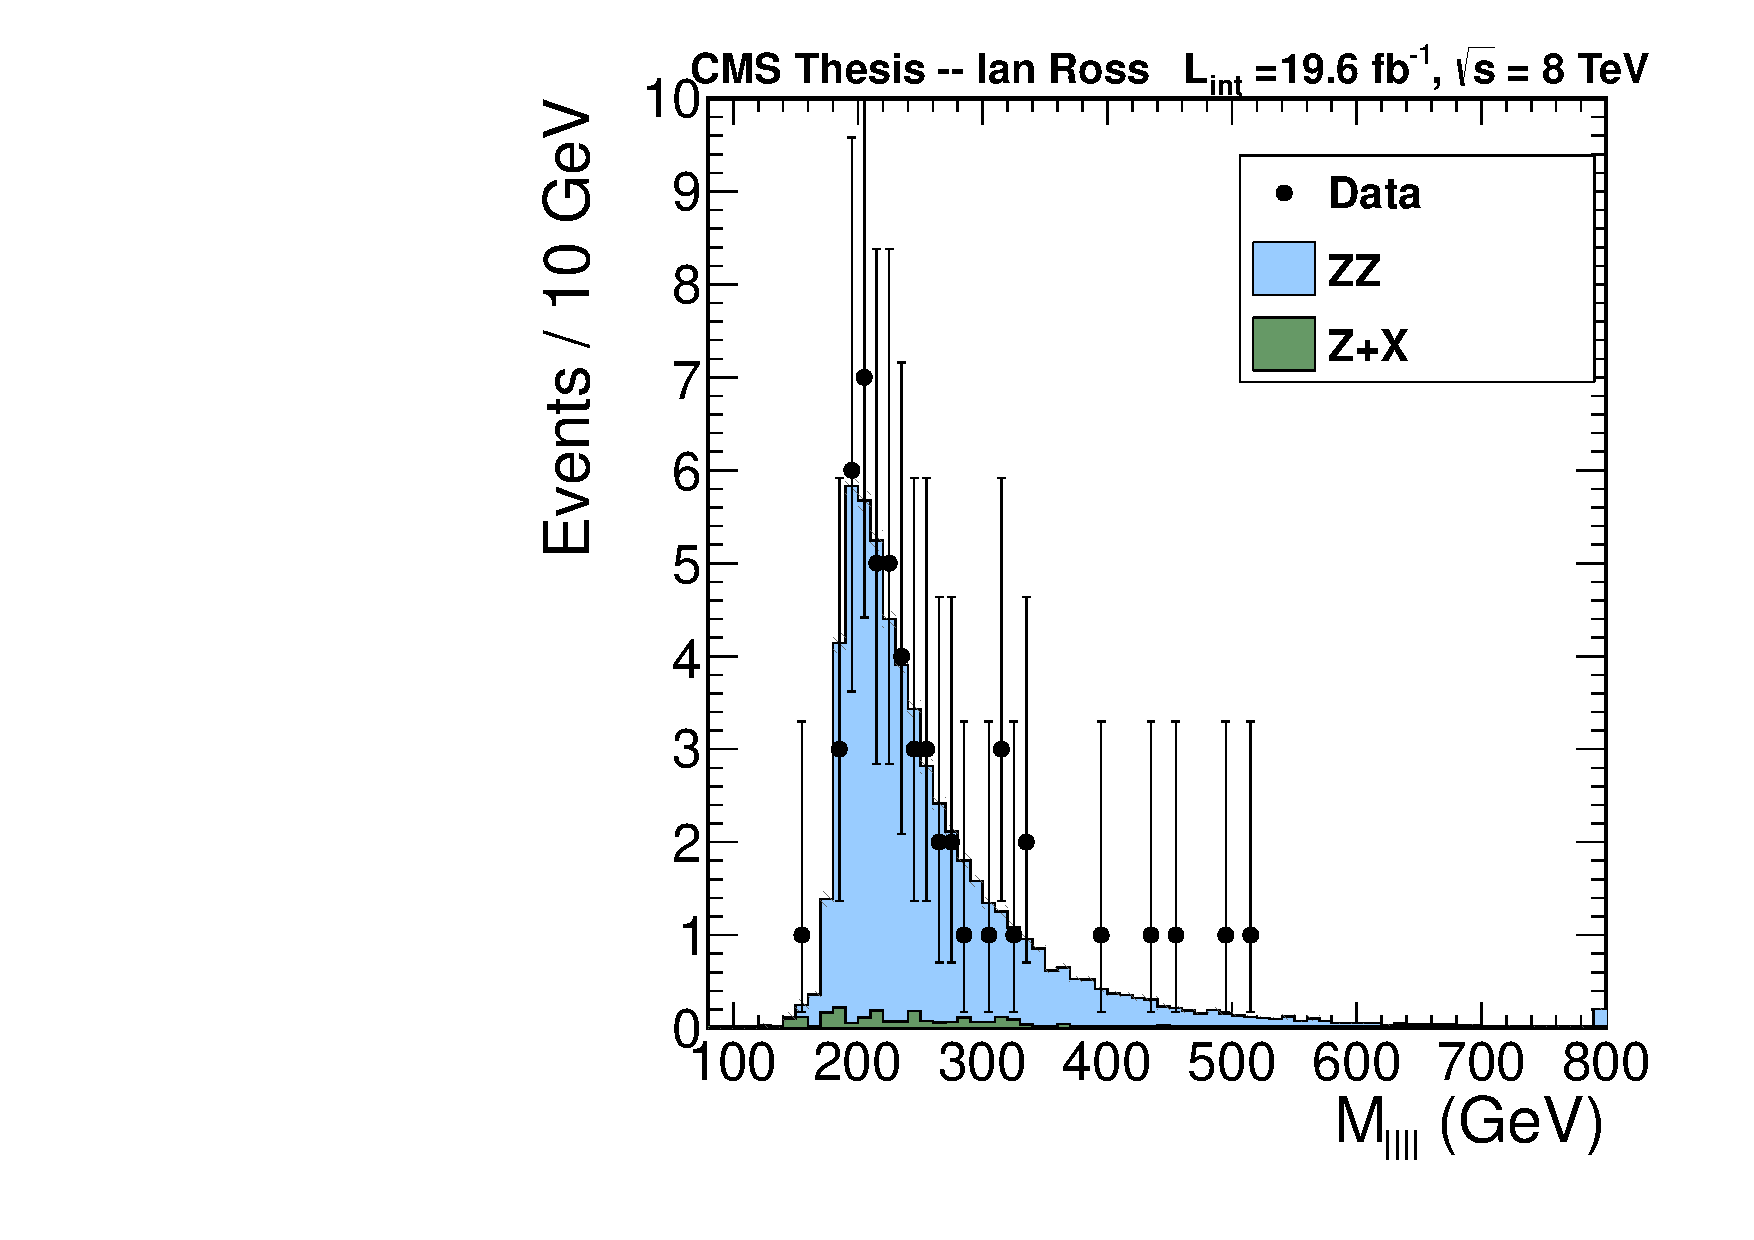
\includegraphics[width=0.40\textwidth]{eeee_mass_highmass}
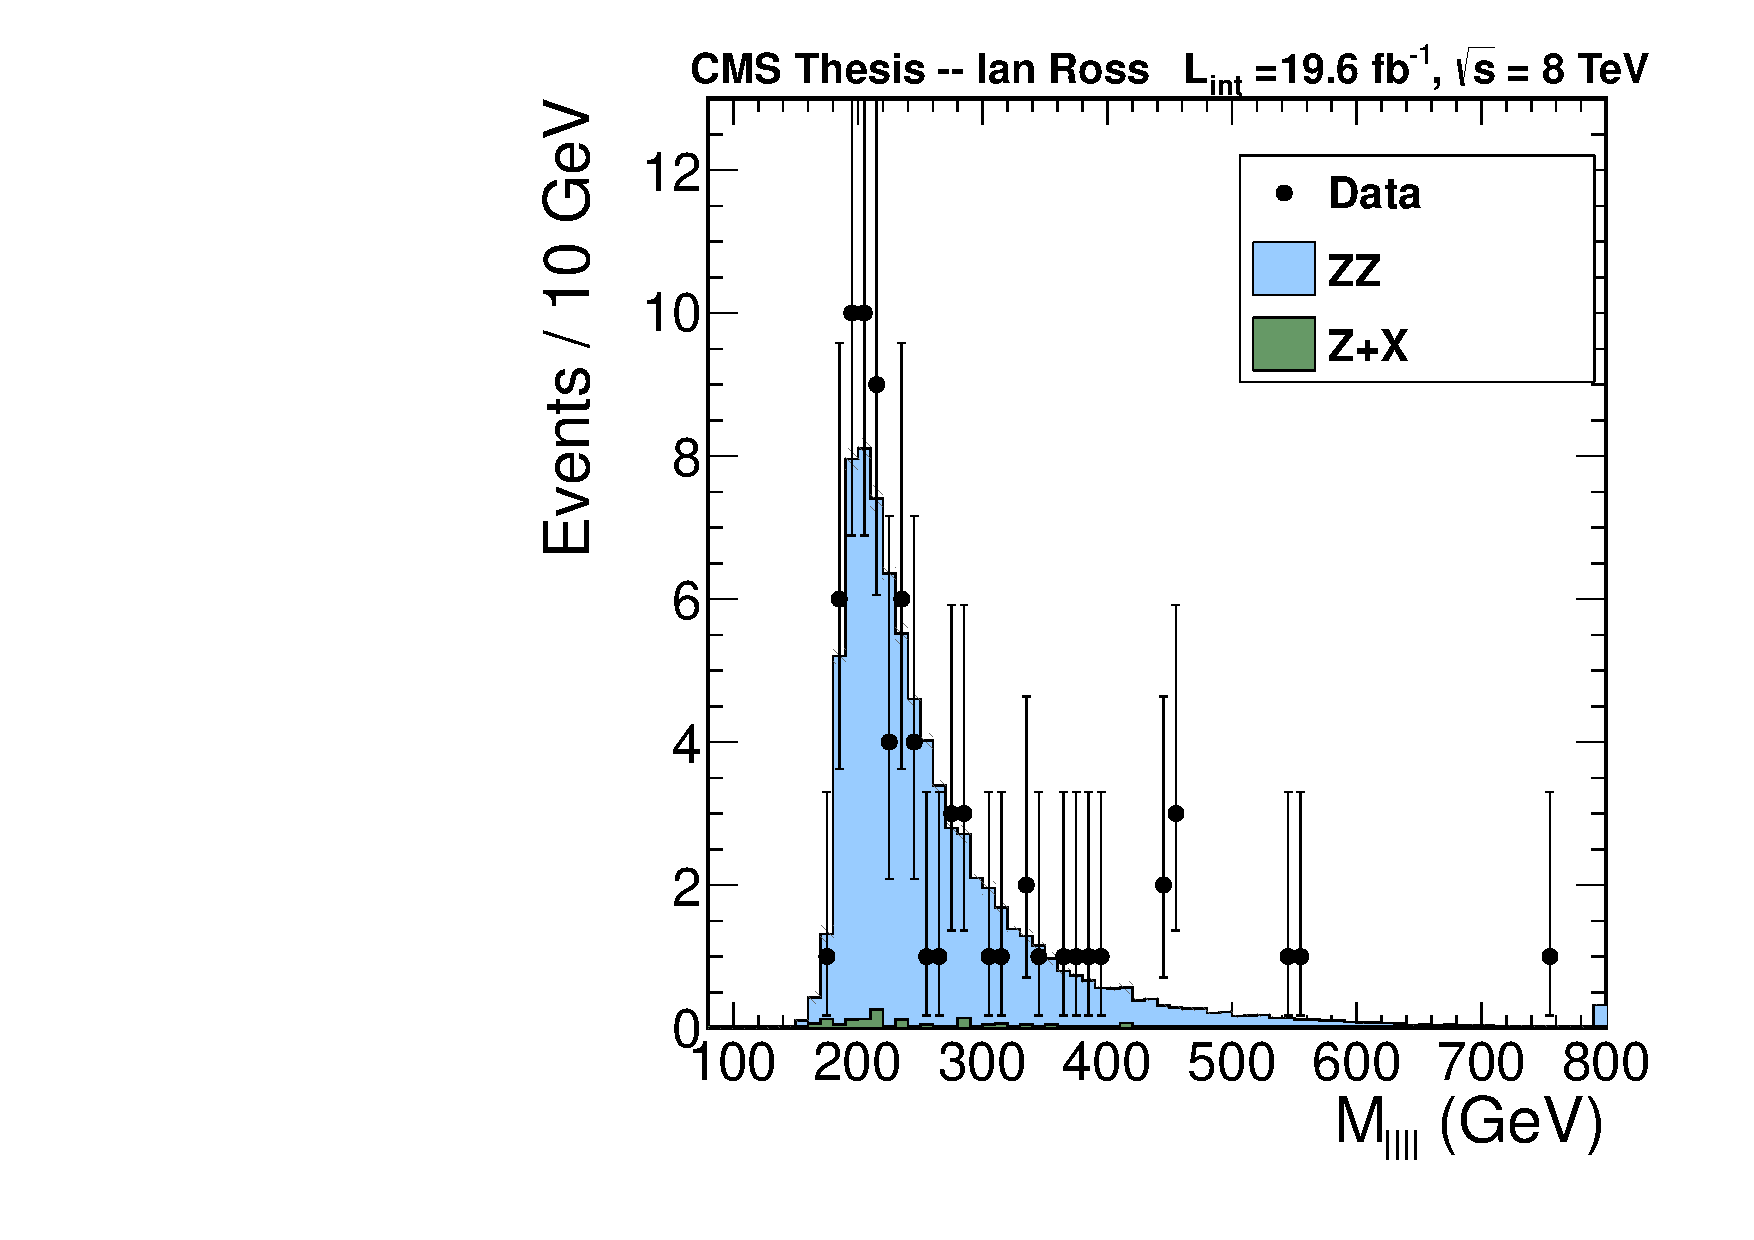
\includegraphics[width=0.40\textwidth]{mmmm_mass_highmass}\\
\includegraphics[width=0.40\textwidth]{eemm_mass_highmass}
\includegraphics[width=0.40\textwidth]{4l_mass_highmass}
\caption[ZZ invariant mass for the high-mass analysis, across the full
considered $M_{\ell\ell\ell\ell}$ range.]{ZZ invariant mass for the high-mass
analysis, across the full considered $M_{\ell\ell\ell\ell}$ range. 
Pictured are
the eeee, $\mu\mu\mu\mu$, $\mu\mu e e$, and combined total results (upper left,
upper right, lower left, and lower right respectively).}
\label{fig:zzMass_high_full}
\end{figure}

\subsection{Cross section measurement} 
The first step of the statistical analysis is to define a likelihood function.
Because we are dealing with a counting experiment in each bin, the natural basis
to use is the Poisson distribution:
\begin{equation}
    f(k; \lambda) =\frac{\lambda^k e^{-k}}{k!} 
\end{equation}
Where $f(k; \lambda)$ is the probability of observing $k$ events, given an
expectation of $\lambda$. In the case of a physics search, k can be defined as:
\begin{equation}
    k = \mu s(\vec{\theta_s}) + b(\vec{\theta_b})
\end{equation}
where $\mu$ is a strength modifier (interpreted as
$\sigma_{measured}/\sigma_{SM}$) on the expected signal, $s$, and $b$ is the
expected background. $\vec{\theta_s}$ and $\vec{\theta_b}$ are the
nuisance parameters associated with the signal and background. These nuisance
parameters enter the expected yields as log-normal constraints.  The total
likelihood, then, is the product of the Poissonian distribution, across all bins
of the histogram:
\begin{equation}
    \label{eqn:likelihood}
    L(\mu, \vec{\theta_s}, \vec{\theta_b}) = \prod f_i(k_i; \lambda_i (\mu,
    \vec{\theta_s}, \vec{\theta_b}))
\end{equation}

The ZZ production cross section is extracted via a simultaneous fit to a likelihood
built from each of the final states. For the case of cross section extraction, a
global counting experiment is used (meaning there is just one bin considered in
Eqn.~\ref{eqn:likelihood} for each final state). 

By maximizing the likelihood function as a function of the signal strength
modifier, $\mu$, one can extract the measured cross section. After removing the
branching ratio of the Z decays into leptons, the ZZ production cross section is
measured as:
\begin{equation}
    \sigma(pp\rightarrow ZZ) = 7.7^{+0.5}_{-0.5} \textrm(stat.) ^{+0.6}_{-0.5}
    \textrm{(sys.)}  \pm 0.3 \textrm{(lumi)} \textrm{pb}
\end{equation}
which agrees favorably with the Standard Model prediction (from MCFM~\cite{MCFM})
of $7.7 \pm 0.6$ pb.
The cross section is also measured using each channel individually. These
results are shown in table~\ref{tab:cross_sections}.

\begin{table}[h]
\centering
\begin{tabular}{|c|c|}
\hline
Final State & $ \sigma(pp \rightarrow ZZ) $ \\
\hline
$\mu\mu\mu\mu$ & 
$    7.3^{+0.8}_{-0.8} \textrm(stat.) ^{+0.7}_{-0.6}
\textrm{(sys.)}  \pm 0.3 \textrm{(lumi)} \textrm{pb} $\\
 eeee & 
    $7.2^{+1.0}_{-0.9} \textrm(stat.) ^{+0.7}_{-0.6}
\textrm{(sys.)}  \pm 0.3 \textrm{(lumi)} \textrm{pb} $\\

$ \mu \mu ee$ & 
    $8.1^{+0.7}_{-0.6} \textrm(stat.) ^{+0.7}_{-0.6}
\textrm{(sys.)}  \pm 0.4 \textrm{(lumi)} \textrm{pb} $\\
Combined & 
    $7.7^{+0.5}_{-0.5} \textrm(stat.) ^{+0.6}_{-0.5}
\textrm{(sys.)}  \pm 0.3 \textrm{(lumi)} \textrm{pb} $\\
\hline
\end{tabular}
\caption[ZZ production cross section measurements for each of the final states
considered and combined.]{ZZ production cross section measurements for each of the final states
considered and combined.}
\label{tab:cross_sections}
\end{table}

\subsection{Unfolding}
In order to remove detector effects from the differential cross sections, the
distributions are \emph{unfolded}. The procedure followed within this analysis
is the iterative Bayesian method, outlined by D'Agostini~\cite{unfolding}.

The measured distribution of a variable is assumed to be a convolved mixture of
the underlying ``true'' distribution and the smearing and distortion resulting
by imperfect detector elements. Specifically, the measured distribution, M, is
related to the true distribution T, through a response matrix, R:
\begin{equation}
    M_i = \sum\limits_j R_{ij} T_j
\end{equation}
The response matrix, $R$, is trained with a Monte Carlo sample,
passing the generated and reconstructed values from each event
into the corresponding (true value, reconstructed value) bin. 
Bayes' theorem is then applied to the elements, using a flat prior, to give the
probability of a true value from bin $i$, given an observation in bin $j$:
\begin{equation}
    P(T_i | M_j) = \frac{P(M_j | T_I) P_0(T_i)}{\sum\limits_{l=1}^{nbins truth}
    P(M_j | T_l) P_0(T_l)}
\end{equation}
And the estimate for the number of true events in bin $i$, is
\begin{equation}
    n_i = \frac{1}{\epsilon_i} \sum\limits_{j=1}^{nbins reco} n_j P(T_i |
    M_J)
\end{equation}
where $\epsilon_i$ is the overall efficiency for reconstructing an event originating
in bin i and $n_j$ is the total number of events observed in bin $j$.
The prior probability, $P_0$ is initially assumed to be flat. However, an
iterative process is used while training, recursively updating the prior until
the predicted and actual true distributions match reasonably well. 

\begin{figure}[h]
\centering
\includegraphics[width=0.45\textwidth]{llll_pt_responseMat}
\includegraphics[width=0.45\textwidth]{llll_mass_responseMat} \\
\includegraphics[width=0.45\textwidth]{leadingLep_pt_responseMat}
\includegraphics[width=0.45\textwidth]{dPhi_Zs_responseMat}
\caption[Example response matrices used in unfolding.]{Example response
matrices used in the unfolding process. Pictured, clockwise from the top left,
are the four-lepton $p_T$, four-lepton mass, leading lepton $p_T$, and azimuthal
separation between the Z bosons. The primarily diagonal nature indicates a
limited number of migrations, due to the excellent detector resolutions.}
\label{fig:responseMatrices}
\end{figure}

The CMS detector has, on the whole, excellent electron and muon
resolution, and as a result there is a limited amount of bin-to-bin migration.
A qualitative example of the unfolded vs. uncorrected distributions are shown in
figure~\ref{fig:unfoldedExample}.
Migrations between bins are slight overall, as are the resulting effects of the
unfolding.
This suggests that the overall detector resolution is excellent, in both
position and momenta measurements, for the objects utilized in the analysis.
Final unfolded differential distributions are presented in
Figures~\ref{fig:unfolding_leadingLepPt},~\ref{fig:unfolding_ZZ},~\ref{fig:unfolding_Z1},and
\ref{fig:unfolding_Z_separation}.

%\begin{figure}[h]
%\centering
%\includegraphics[width=0.40\textwidth]{placeholder}
%\includegraphics[width=0.40\textwidth]{placeholder} \\ 
%\includegraphics[width=0.40\textwidth]{placeholder}
%\includegraphics[width=0.40\textwidth]{placeholder} \\ 
%\includegraphics[width=0.40\textwidth]{placeholder}
%\includegraphics[width=0.40\textwidth]{placeholder} 
%\caption[Measured electron and muon resolutions (with comparison to generated
%resolutions).]{Measured electron and muon resolutions, with comparisons to
%generated resolutions. Muons (left) and electrons (right) both show excellent
%detector response in $p_{T}, \eta, \textrm{and} \phi$ (top, middle, and bottom
%respectively).}
%\label{fig:objectResolution}
%\end{figure}

\begin{figure}[h]
\centering
\includegraphics[width=0.80\textwidth]{dPhi_Zs_comp}
\caption[An example of the effects of unfolding.]{An example of the effects of
    unfolding. The $\Delta \phi$ separation between Z candidates is relatively
    unchanged by the unfolding (red, measured, and black, unfolded, are nearly
    identical).}
\label{fig:unfoldedExample}
\end{figure}
%%%%

\begin{figure}[h]
\centering
\includegraphics[width=0.75\textwidth]{leadingLep_pt}
\caption[Unfolded distribution of the highest $p_T$ lepton.]{Unfolded
distribution of the highest lepton $p_T$.}
\label{fig:unfolding_leadingLepPt}
\end{figure}

\begin{figure}[h]
\centering
\includegraphics[width=0.75\textwidth]{llll_pt} \\
\includegraphics[width=0.75\textwidth]{llll_mass}
\caption[Unfolded ZZ kinematic variables.]{Unfolded ZZ kinematic variables. The
ZZ system $p_{T}$ (top) and $M_{\ell\ell\ell\ell}$ (bottom).}
\label{fig:unfolding_ZZ}
\end{figure}

\begin{figure}[h]
\centering
\includegraphics[width=0.75\textwidth]{llll_leadingZpt} \\ 
\includegraphics[width=0.75\textwidth]{llll_leadingZeta}
\caption[Unfolded leading (in $p_T$) Z kinematic variables.]{Unfolded leading (in
$p_T$) kinematic variables. The unfolded
Z system $p_{T}$ (top) and $\eta$ (bottom) distributions.}
\label{fig:unfolding_Z1}
\end{figure}

\begin{figure}[h]
\centering
\includegraphics[width=0.75\textwidth]{dPhi_Zs} \\ 
\includegraphics[width=0.75\textwidth]{llll_dR_Z}
\caption[Unfolded distribution of the Z candidate separation.]{Unfolded
distribution of the Z candidate separations, $\Delta \phi$ top and $\Delta R$
bottom.}
\label{fig:unfolding_Z_separation}
\end{figure}


\clearpage

\section{Search for a Standard Model Higgs Boson}
Overall yields for the low-mass (Higgs search) analysis are presented in
Table~\ref{tab:higgsYields}. The observed four-lepton invariant mass across the
entire mass range is presented in Figure~\ref{fig:zzMass_higgs_full}. A
significant excess is observed in the vicinity of 126~GeV, and this region is
shown in finer binning in Figure~\ref{fig:zzMass_higgs_low}.

\begin{table}[h]
\centering
\begin{tabular}{|c|c|c|c|}
\hline
& eeee & $\mu\mu\mu\mu$ & $\mu\mu e e$ \\
\hline
H(126) & $2.86\pm0.03$ & $5.49 \pm 0.05$ & $7.92 \pm 0.06$ \\
H(350) & $11.65 \pm 0.09 $ & $15.80\pm 0.11$ & $27.89 \pm 0.15$ \\
ZZ & $ 68.21 \pm 0.29 $ & $ 101.58 \pm 0.39 $ & $ 167.32 \pm 0.66 $ \\
Z+Jets & $6.70 \pm 0.49$ & $3.46 \pm 0.78$ & $7.82 \pm 0.80$ \\
\hline
BG Expected & 74.91 & 105.04 & 175.14 \\
\hline
Observed & 73 & 109 & 194 \\
\hline
\end{tabular}
\caption[Final yields per event channel in the low-mass analysis (search for the
Higgs boson).]{Final yields per event channel in the low-mass analysis (search for the
Higgs boson). Errors are statistical only.} 
\label{tab:higgsYields}
\end{table}

\begin{figure}[h]
\centering
\includegraphics[width=0.40\textwidth]{eeee_mass_full}
\includegraphics[width=0.40\textwidth]{mmmm_mass_full}\\
\includegraphics[width=0.40\textwidth]{eemm_mass_full}
\includegraphics[width=0.40\textwidth]{4l_mass_full}
\caption[ZZ invariant mass for the low-mass analysis, across the full considered
$M_{\ell\ell\ell\ell}$ range.]{ZZ invariant mass for the low-mass analysis, across the full considered
$M_{\ell\ell\ell\ell}$ range. 
Pictured are the eeee, $\mu\mu\mu\mu$, $\mu\mu e
e$, and combined total results (upper left, upper right, lower left, and lower
right respectively).}
\label{fig:zzMass_higgs_full}
\end{figure}

\begin{figure}[h]
\centering
\includegraphics[width=0.40\textwidth]{eeee_mass_low}
\includegraphics[width=0.40\textwidth]{mmmm_mass_low}\\
\includegraphics[width=0.40\textwidth]{eemm_mass_low}
\includegraphics[width=0.40\textwidth]{4l_mass_low}
\caption[ZZ invariant mass including the low-mass $ZZ*$ analysis, zoomed to take a closer
look at the excess.]{ZZ invariant mass including the low-mass $ZZ*$ analysis, zoomed to take
a closer look at the excess. Pictured are
the eeee, $\mu\mu\mu\mu$, $\mu\mu e e$, and combined total results (upper left,
upper right, lower left, and lower right respectively).}
\label{fig:zzMass_higgs_low}
\end{figure}

\subsection{Statistical Analysis}
A test statistic, $q_\mu$, based on the likelihood function defined
in~\ref{eqn:likelihood}, is defined to extract upper limits:
\begin{equation}
    \tilde{q_\mu} = -2 \ln \frac{L (\mu, \vec{\theta_{s \mu}}, \vec{\theta_{b \mu}})}{L(\hat \mu,
    \hat{\vec{ \theta_{s}}}, \hat{\vec{ \theta_{b}}})}
\end{equation}
where $\hat \theta_{i \mu}$ are the conditional maximum likelihood estimators,
and $\hat \mu$, $\hat \theta_s$, and $\hat \theta_b$ are the parameters which
maximize the global likelihood.
From here, probability density functions are built for signal-plus-background
and background-only hypotheses. From these, p-values for the both scenarios are
calculated:
\begin{equation}
    p_\mu = P(\tilde{q_\mu} \ge \tilde{q_\mu^{obs}} |
    \textrm{signal+background})
\end{equation}
\begin{equation}
    1-p_b = P(\tilde{q_\mu} \ge \tilde{q_\mu^{obs}} |
    \textrm{background only})
\end{equation}
corresponding to the probability of observing a test statistic at least as large
as that observed, given a signal-plus-background or background only hypothesis.
Finally, the CLs value is defined to be the ratio between these probabilities:
\begin{equation}
    CLs = \frac{p_\mu}{1-p_b}
\end{equation}
The CLs value has the property that, given a value of $\mu$ and CLs value $\le
\alpha$, a Higgs of that signal strength is excluded at the $1-\alpha$
confidence level. Thus, to set a 95\% confidence level upper limit, the value of
$\mu$ is adjusted until the CLs value is 0.05.

Similarly, in order to find the significance of an observation, a test statistic
$q_0$ is defined:
\begin{equation}
    q_0 = -2 \ln \frac{L (0, \vec{\theta_{s 0}}, \vec{\theta_{b 0}})}{L(\hat \mu,
    \hat{\vec{ \theta_{s}}}, \hat{\vec{ \theta_{b}}})}
\end{equation}
Again, a pdf is constructed using pseudo-data and a background-only hypothesis,
and a p-value for the observed test statistic is constructed:
\begin{equation}
    p_\mu = P(q_0 \ge q_0^{obs})
\end{equation}
The corresponding significance of this p-value is taken from a normal one-sided
hypothesis scenario.  A full suite of tools has been developed in CMS to provide
the statistical framework for the search for the Higgs boson\cite{higgsStats}.

A local p-value scan is done across the full mass range, Figure~\ref{fig:pvals},
with a maximum local significance of $6.1\sigma$ observed at a Higgs mass of
126~GeV. 95\% confidence level upper limits are calculated from 110~GeV up to
1~TeV, excluding a Standard Model Higgs boson in the ranges of 130 to 600~GeV.   

\begin{figure}[h]
\centering
\includegraphics[width=0.45\textwidth]{higgs_limits_full}
\includegraphics[width=0.45\textwidth]{higgs_limits_low} \\
\caption[95\% CL Upper Limits on Standard Model Higgs production.]{95\% CL Upper
Limits on Standard Model Higgs production (full mass range on the left, with a
low-mass scan on the right).}
\label{fig:higgsLimits}
\end{figure}

\begin{figure}[h]
\centering
\includegraphics[width=0.45\textwidth]{pvals_full} 
\includegraphics[width=0.45\textwidth]{pvals_low}\\
\caption[p-value scan.]{p-value scan for the full (left) and low (right) mass
ranges.}
\label{fig:pvals}
\end{figure}

\clearpage % get all the Higgs stuff dumped

\section{Limits on anomalous triple gauge couplings}
In order to set limits on the neutral triple gauge couplings, a binned counting
procedure is followed. First, a $3\times3$ grid of ($f_i^Z, f_i^\gamma$) Monte
Carlo simulations are generated in SHERPA~\cite{SHERPA} and fully simulated and
reconstructed. Because one of the major implications of the existence of
anomalous couplings is an enhanced high-mass tail in $M_{\ell \ell\ell\ell}$,
this variable is chosen as the discriminating variable. For each of the
generated samples, the $M_{\ell\ell\ell\ell}$ is plotted (using the same binning
for all samples). Yields in intermediary points in the coupling space are
interpolated bin-by-bin using a paraboloid fit to the existing samples, as
Fermi's Golden Rule suggests a quadratic dependence on cross section. A
likelihood for the null and alternative hypotheses is built, just like in the
Higgs case outlined above. However, in the case of the triple gauge coupling
limits, the CLs methodology is not used. Instead, a simple likelihood profiling
is used, using Wilks' theorem to set the confidence levels. The CLs limit %TODO:ref
procedure is not used because, by definition, it will never exclude the null
hypothesis. Given the presence of non-SM values of the couplings, the CLs limits
give limits which have little utility.

The invariant mass of the four-lepton system contains little information about
the sign of the couplings involved. The resulting likelihood scan shows this
degeneracy (Figure~\ref{fig:atgc_likelihood}), suggesting that only the size, but
not the sign, of the couplings could be extracted from this information.

\begin{figure}[h]
\centering
\includegraphics[width=0.80\textwidth]{contCanvas_fakeData.pdf}
\caption[Qualitative likelihood scan of the ($f_4^Z, f_4^{\gamma}$) coupling
space, with a signal injected.]{A qualitative
likelihood scan of the ($f_4^Z, f_4^\gamma$) coupling space, with an aTGC signal
injected. The degeneracy suggests that measurement of the sign of the couplings
would be impossible using just the information from the four-lepton invariant
mass.}
\label{fig:atgc_likelihood}
\end{figure}

Though SHERPA is a leading-order generator, it has been shown (see
Figure~\ref{fig:sherpaPowhegComp}) that SHERPA generation (with up to one extra
parton interaction) accurately reproduces the invariant mass kinematics of the
NLO POWHEG generation. This gives confidence that the differences between LO and
NLO in the discriminating variable ($M_{\ell\ell\ell\ell}$) are slight, and
SHERPA is an acceptable generator for the aTGC sample generation.

\begin{figure}[h]
\centering
\includegraphics[width=0.80\textwidth]{sherpa_powheg_comp}
\caption[Comparison of the $M_{\ell\ell\ell\ell}$ for Standard Model ZZ production
by the LO generator SHERPA and the NLO POWHEG.]{Comparison of the
    $M_{\ell\ell\ell\ell}$ shape from Standard Model ZZ production by the LO generator
    SHERPA and the NLO POWHEG. Differences are slight, justifying the use of
SHERPA in generating the aTGC Monte Carlo samples. The last bin contains the
overflow of all higher $M_{\ell\ell\ell\ell}$ values.} 
\label{fig:sherpaPowhegComp}
\end{figure}

No significant deviation from the Standard Model expectations are observed, and
95\% Confidence Level upper limits are set using profile likelihood methodology.
Limits are extracted for the two dimension $(f_4^Z, f_4^{\gamma})$ and $(f_5^Z,
f_5^{\gamma})$ coupling spaces separately (with the other two couplings held to
0). Additionally, single-coupling limits are calculated by restricting the other
couplings to 0. The two- and one-dimensional limits are depicted in
Figure~\ref{fig:atgc_limits}, and the one-dimensional limits are presented in
Table~\ref{tab:atgc_limits}.

\begin{figure}[h]
\centering
\includegraphics[width=0.45\textwidth]{lim_f4z_f4g}
\includegraphics[width=0.45\textwidth]{lim_f5z_f5g}
\caption[2D limits on the neutral anomalous triple gauge couplings.]{2D limits
on the neutral anomalous triple gauge couplings. The solid line represents the 95\%
confidence level on the 2D coupling, the dashed line represents the 68\%
confidence level, and the red lines represent the 95\% confidence level
limits (with the other couplings constrained to 0). The block dot represents the
best-fit coupling values.}
\label{fig:atgc_limits}
\end{figure}

\begin{table}[h]
\centering
\begin{tabular}{|c|c|c|}
    \hline
i  & $f_{i}^Z $& $f_{i}^{\gamma} $ \\
\hline
$4$ & $-0.004 < f_4^Z < 0.004 $&$ -0.005 < f_4^{\gamma} < 0.005 $\\
$5$ & $-0.004 < f_5^Z < 0.004 $&$ -0.005 < f_5^{\gamma} < 0.005 $\\
\hline
\end{tabular}
\caption[1D limits on the neutral anomalous triple gauge couplings.]{1D limits
on the neutral anomalous triple gauge couplings. Values are extracted by holding
the other three neutral couplings to 0.}
\label{tab:atgc_limits}
\end{table}
\clearpage


\chapter{Conclusions}
\label{chapter:conclusions}
\section{Summary}

A search for a Standard Model-like Higgs boson and anomalous neutral triple
gauge couplings has been conducted at $\sqrt{s} = 8~TeV$, using 19.6~\fbinv of
pp collision data. The analysis benefits greatly from having a clean signature,
allowing the usage of highly efficient reconstruction and selection algorithms
while maintaining a low level of reducible background. This background was
estimated using an entirely data-driven process, while the Standard Model ZZ
production and Higgs signal processes were simulated using Monte Carlo methods.

The search for a Standard Model Higgs boson in the $H\rightarrow ZZ\rightarrow
\ell\ell\ell\ell$ final state resulted in a discovery of a new boson, with a
6.1$\sigma$ excess at a hypothesized Higgs mass of 126~GeV. 

A search for the anomalous neutral triple gauge couplings \ffour and \ffive was
conducted. The results are fully consistent with Standard Model behaviour, and
95\% confidence level upper limits were set on the coupling strengths. The cross
section for Standard Model $ZZ\rightarrow\ell\ell\ell\ell$ production was
measured from the collected data, showing excellent agreement with theoretical
calculations.


\section{Future Outlook}
Looking toward the future, the properties of the new boson, the differential
cross sections of Standard Model ZZ production, and the continued search for
anomalous triple gauge couplings will all benefit from the increased cross
sections and luminosity expected from the LHC upgrades currently under way.
Increases in center-of-mass energies from 8~TeV to 13 or 14~TeV along with a
projected data collection of ${\sim500}$\fbinv by the end of the decade will
result in unprecedented precision in all ${(H\rightarrow)ZZ\rightarrow
\ell\ell\ell\ell}$ measurements.

The clean nature of the channel in addition to its fully reconstructed final
state allow an excellent handle on doing further analysis of the newly discovered
boson. An extension of the matrix element kinematic discriminant can be used to
comb out the likely spin properties, while creating a separate category for
events produced via Vector Boson Fusion (which includes a forward jet signature)
can be used to measure the relative fermionic and vector boson couplings. 



\bibliography{bibliography}{}
\bibliographystyle{unsrt}

\end{document}
